%========================================================
% DOCUMENT PREAMBLE
%========================================================

\documentclass[a4paper]{article}

%--------------------------------------------------------
% Language and font encodings
%--------------------------------------------------------
\usepackage[english]{babel}
\usepackage[utf8]{inputenc}
\usepackage[T1]{fontenc}
\usepackage{amsfonts}

%--------------------------------------------------------
% Page layout
%--------------------------------------------------------
\usepackage[
a4paper,
top=3cm,
bottom=2cm,
left=3cm,
right=3cm,
marginparwidth=2cm
]{geometry}

%--------------------------------------------------------
% Mathematical and general packages
%--------------------------------------------------------
\usepackage{amsmath}
\usepackage{amssymb}
\usepackage{amsthm}
\usepackage{caption}
\usepackage{subcaption}
\usepackage[english]{babel}
\usepackage{datetime2}

\usepackage{graphicx}
\usepackage[section]{placeins}

\usepackage[colorinlistoftodos]{todonotes}
\usepackage[colorlinks=true, allcolors=blue]{hyperref}

%--------------------------------------------------------
% Section formatting
%--------------------------------------------------------
\usepackage{titlesec}
\usepackage{ragged2e}

\titleformat{\section}
  {\normalfont\Large\bfseries\RaggedRight}
  {\thesection}
  {1em}
  {}

\titleformat{\subsection}
  {\normalfont\large\bfseries\RaggedRight}
  {\thesubsection}
  {1em}
  {}

\newcommand{\sectionbreak}{\clearpage}

%--------------------------------------------------------
% Tables
%--------------------------------------------------------
\usepackage{array}
\newcolumntype{P}[1]{>{\centering\arraybackslash}p{#1}}
\usepackage{multirow}

%--------------------------------------------------------
% Title metadata
%--------------------------------------------------------
\title{
Mathematical and Physical Modeling of Entangled Photon Propagation in Optical Fibers for MATLAB Simulation
}

\author{
Marco Cioci\\
Politecnico di Milano\\
Student ID: 10694772\\
\texttt{marco.cioci@mail.polimi.it}
}

\date{\DTMenglishmonthname{\the\month}, \the\year}

%--------------------------------------------------------
% Global formatting
%--------------------------------------------------------
\setlength{\parindent}{0pt}

%========================================================
% DOCUMENT START
%========================================================

\begin{document}

\maketitle

\tableofcontents

\medskip


%========================================================
% SECTION 1 — General Framework
%========================================================

\newpage
\section{General Framework}

%--------------------------------------------------------
% Subsection 1.1 — Purpose and Scope
%--------------------------------------------------------

\subsection{Purpose and Scope}

The purpose of this document is to define a coherent working framework for the mathematical modeling and numerical simulation of polarization-entangled photon pairs propagating through optical fibers.

This text is not intended to appear directly in the final thesis manuscript. Instead, it serves as an internal technical guide throughout the development of the project. Its role is to support communication, maintain consistency of notation and assumptions, and provide a stable reference for the progressive validation of both the theoretical model and the MATLAB implementation.

\medskip

The central objective is to organize the physical assumptions, mathematical formalism, and simulation strategy into a reproducible structure, so that each computational step can be traced back to a precise theoretical element. In this way, the simulator is not developed as an isolated numerical tool, but as a direct operational translation of the underlying quantum model.

\medskip

\paragraph{Implementation.}

At the MATLAB level, this document should be treated as the reference specification for notation, model hierarchy, and implementation priorities.

The simulator is therefore organized into clearly identifiable modules, each corresponding to a specific theoretical block. This modular structure enables step-by-step validation of intermediate results and supports systematic extensions of the model.

Implementation remarks are included only where the mapping from theory to computation is non-trivial, in order to preserve clarity and avoid redundancy.

%--------------------------------------------------------
% Subsection 1.2 — Theoretical Formalism and Notation
%--------------------------------------------------------

\subsection{Theoretical Formalism and Notation}

The system is described within the framework of quantum information theory. The relevant mathematical structures include finite-dimensional Hilbert spaces, quantum states, tensor products, unitary operators, density operators, and projective measurements.

Elements of classical optics are introduced only when required to justify the physical origin of the effective quantum transformations.

\medskip

The notation and formal tools are aligned, as far as possible, with the framework of \textit{Quantum Computation and Quantum Information} by Nielsen and Chuang.

\medskip

In this formalism:
\begin{itemize}
\item single subsystems are represented by vectors in \( \mathbb{C}^2 \),
\item composite systems are described by tensor-product spaces,
\item evolutions are represented by linear operators (unitary in the ideal case),
\item measurements are described through Hermitian operators.
\end{itemize}

\medskip

All states and operators are represented as vectors and matrices over \( \mathbb{C} \), with dimensions determined by the tensor-product structure of the system.

\medskip

\paragraph{Implementation.}

The simulator adopts a quantum-information-oriented representation from the outset.

Pure states are represented as complex vectors, mixed states as density matrices, and evolutions and measurements as matrix operators.

This abstract structure defines the numerical backbone of the simulator and is independent of the specific physical encoding used.

%--------------------------------------------------------
% Subsection 1.3 — Physical Scenario and Experimental Setting
%--------------------------------------------------------

\subsection{Physical Scenario and Experimental Setting}

The physical setting considered in this work is the following.

A spontaneous parametric down-conversion (SPDC) source generates pairs of
polarization\-entangled photons, ideally prepared in a Bell state. The two photons
are injected into distinct optical paths, denoted \(A\) and \(B\), and propagate
through independent optical fibers.

\medskip

Each fiber acts on the polarization degree of freedom of the corresponding photon. In a general description, this action can be represented by a unitary operator acting on a single-qubit Hilbert space.

However, motivated by experimental constraints and by the limited degree of control available on the full polarization transformation, the model is initially restricted to a simplified effective description.

\medskip

After compensation of global polarization rotations, the dominant residual effect can be modeled as a relative phase shift between the horizontal and vertical polarization components.

In the qubit representation, this corresponds to a rotation around the computational \( Z \)-axis of the Bloch sphere.

\medskip

The objective at this stage is therefore not to reproduce the full electromagnetic propagation in optical fibers, but to construct an effective quantum model that captures the relevant impact of fiber propagation on entanglement and measurable correlations.

\medskip

\paragraph{Implementation.}

At the simulator level, the physical scenario is reduced to the minimal set of elements required for computation:

\begin{itemize}
\item an initial bipartite quantum state,
\item two labeled channels \( A \) and \( B \),
\item one local transformation acting on each subsystem.
\end{itemize}

\medskip

In the first modeling stage, unnecessary optical detail is neglected and each fiber is described exclusively through its effective action on polarization.

This leads to a local unitary representation of the form

\[
U_A \otimes U_B
\]

where \( U_A, U_B \in \mathbb{C}^{2 \times 2} \) are unitary operators.

\medskip

This abstraction defines the fundamental interface between the physical system and the simulator, and will later allow the introduction of more refined models, including stochastic phase evolution and non-unitary effects.


%========================================================
% SECTION 2 — Modeling Strategy
%========================================================

\section{Modeling Strategy}

%--------------------------------------------------------
% Subsection 2.1 — Progressive Modeling Approach
%--------------------------------------------------------

\subsection{Progressive Modeling Approach}

The modeling approach follows a progressive refinement strategy, in which the system is described through successive levels of approximation of increasing physical complexity.

Each stage introduces additional physical effects while remaining consistent with the previous ones. This ensures analytical transparency and preserves continuity between simplified and refined models.

\medskip

From a theoretical perspective, this approach isolates the contribution of individual mechanisms. From a computational perspective, it enables a layered simulator structure, where each refinement corresponds to a well-defined extension of the existing codebase.

\medskip

%--------------------------------------------------------
% Subsection 2.2 — Hierarchy of Modeling Levels
%--------------------------------------------------------

\subsection{Hierarchy of Modeling Levels}

The modeling workflow is structured as a sequence of progressively refined descriptions:

\[
\begin{array}{c}
\text{Ideal Bell State} \\
\downarrow \\
\text{Local Phase Model (Z-rotations)} \\
\downarrow \\
\text{General Local Unitary Transformations} \\
\downarrow \\
\text{Mixed-State Description (Density Operators)} \\
\downarrow \\
\text{Noisy Quantum Channels} \\
\downarrow \\
\text{Effective Fiber Models}
\end{array}
\]

\medskip

More explicitly:

\begin{itemize}

\item \textbf{Level 1: Minimal phase model}  
Pure, maximally entangled state with fiber action reduced to a relative phase. This level captures the analytical dependence of correlation observables on a single parameter.

\item \textbf{Level 2: General unitary dynamics}  
Arbitrary polarization rotations described by local operators \( U_A \otimes U_B \).

\item \textbf{Level 3: Mixed-state description}  
Density operators used to represent statistical mixtures and loss of coherence.

\item \textbf{Level 4: Noisy quantum channels}  
Effective completely positive trace-preserving (CPTP) maps modeling depolarization and decoherence.

\item \textbf{Level 5: Effective fiber models}  
Physically motivated descriptions, such as concatenations of random unitary segments or stochastic polarization evolution.

\end{itemize}

\medskip

This hierarchy provides both a conceptual and an implementation roadmap. The initial levels remain analytically tractable and allow direct validation, while the later levels increase physical realism and connect to experimentally relevant effects.

\medskip

\paragraph{Implementation.}

This hierarchical structure should be mirrored explicitly in the codebase. Each level corresponds to a distinct layer of functionality, including state preparation, local unitary evolution, density-matrix handling, channel application, and advanced propagation models.

This ensures that each refinement is introduced as an additional computational step, preserving modularity and avoiding structural modifications of previously validated components.

%--------------------------------------------------------
% Subsection 2.3 — Baseline Model: Pure-State Description
%--------------------------------------------------------

\subsection{Baseline Model: Pure-State Description}

At the first stage, the bipartite system is described as a pure state in \( \mathbb{C}^2 \otimes \mathbb{C}^2 \), and fiber propagation is modeled through local unitary transformations. Particular emphasis is placed on relative phase shifts induced by the fibers.

\medskip

The main objective is to analyze how these phase shifts affect measurable two-photon correlations. The relevant observables are operators of the form
\[
\sigma_i \otimes \sigma_j,
\qquad i,j \in \{x,y,z\},
\]
as well as operators corresponding to arbitrary measurement directions on the Bloch sphere.

\medskip

This baseline model constitutes the simplest regime in which entanglement is preserved and can be probed exclusively through correlation observables. It provides a controlled setting for deriving analytical expressions and validating the numerical implementation.

\medskip

\paragraph{Implementation.}

At this level, the simulator operates on pure two-qubit states represented as \( 4 \times 1 \) complex vectors.

The core tasks are:
\begin{itemize}
\item generation of the Bell state,
\item application of local operators \( U_A \) and \( U_B \),
\item evaluation of expectation values.
\end{itemize}

In this regime, the simulator enables direct comparison between analytical predictions and numerical results for correlation functions, establishing a first level of validation that will be extended in Chapter~4 through quantitative state characterization.

%--------------------------------------------------------
% Subsection 2.4 — Extension to Mixed-State Formalism
%--------------------------------------------------------

\subsection{Extension to Mixed-State Formalism}

At the next level, the model incorporates statistical effects and decoherence. In this regime, the pure-state description is no longer sufficient and must be replaced by a density-operator formalism.

\medskip

This extension enables the description of:
\begin{itemize}
\item reduced states of individual photons,
\item loss of coherence due to unresolved degrees of freedom,
\item effective non-unitary dynamics arising from environmental interactions or statistical averaging.
\end{itemize}

\medskip

Within this framework, physically relevant quantities such as purity, fidelity, and concurrence can be defined and computed, allowing a quantitative characterization of mixedness and entanglement (see Chapter~4).

\medskip

An important derived quantity is the reduced density operator of a subsystem, obtained via partial trace. For instance, the reduced state of subsystem \( A \) is
\[
\rho_A = \mathrm{Tr}_B(\rho_{AB}).
\]

For maximally entangled states such as \( |\Psi^+\rangle \), the reduced density operators are maximally mixed:
\[
\rho_A = \rho_B = \frac{1}{2} I.
\]

\medskip

This property reflects the absence of local information despite strong nonlocal correlations, and provides the conceptual link between entanglement and mixedness that will be explored quantitatively in later sections.

\medskip

Expectation values in the density-operator formalism are computed as
\[
\langle O \rangle = \mathrm{Tr}(\rho O),
\]
which generalizes the pure-state expression \( \langle \psi | O | \psi \rangle \).

\medskip

\paragraph{Implementation.}

The simulator must be extended so that all routines operate on density matrices, including \( 4 \times 4 \) representations, partial trace operations, and observable evaluation.

This generalized framework enables the transition from deterministic evolution to ensemble-based descriptions and supports the computation of state metrics used for validation and physical interpretation.

The pure-state implementation is preserved as a special case, ensuring consistency across all modeling levels.

%--------------------------------------------------------
% Subsection 2.5 — Simulator Design and Architecture
%--------------------------------------------------------

\subsection{Simulator Design and Architecture}

The simulator is designed as a modular implementation of the theoretical model.

\medskip

The initial modules include:
\begin{itemize}
\item Bell-state generation,
\item local unitary propagation,
\item correlation evaluation.
\end{itemize}

\medskip

More advanced modules introduce:
\begin{itemize}
\item quantum channels,
\item reduced density operators,
\item entanglement measures,
\item experimentally relevant observables such as Bell parameters and Stokes-like quantities.
\end{itemize}

\medskip

The theoretical structure is directly reflected in the computational architecture, ensuring consistency, traceability, and extensibility.

The implementation distinguishes clearly between reusable computational kernels and higher-level experiment scripts, allowing the simulator to evolve into a structured and reusable research tool.

\medskip

\paragraph{Implementation.}

At the current stage, this modular design is reflected in the directory structure:
\begin{itemize}
\item \texttt{Core}: state vectors, operators, expectation values, correlation routines;
\item \texttt{Models}: physical propagation models;
\item \texttt{Utils}: validation routines and auxiliary tools;
\item \texttt{Experiments}: scripts implementing complete simulation studies.
\end{itemize}

This separation enforces a strict distinction between general mathematical operations and physically specific modeling choices.


%========================================================
% SECTION 3 — Physical and Mathematical Representation
%========================================================

\section{Physical and Mathematical Representation}

%--------------------------------------------------------
% Subsection 3.1 — Quantum System and Hilbert Space Structure
%--------------------------------------------------------

\subsection{Quantum System and Hilbert Space Structure}

The physical system considered consists of polarization-entangled photon pairs generated by spontaneous parametric down-conversion (SPDC). The two photons propagate along distinct paths, denoted \(A\) and \(B\), forming a bipartite system.

In this work, the qubit is encoded in the polarization degree of freedom:
\[
|H\rangle \equiv |0\rangle,
\qquad
|V\rangle \equiv |1\rangle.
\]

Accordingly, the computational basis of the bipartite system is
\[
\{
|00\rangle,\,
|01\rangle,\,
|10\rangle,\,
|11\rangle
\},
\]
corresponding to
\[
\{
|H\rangle_A |H\rangle_B,\,
|H\rangle_A |V\rangle_B,\,
|V\rangle_A |H\rangle_B,\,
|V\rangle_A |V\rangle_B
\}.
\]

The Hilbert space of the total system is therefore
\[
\mathcal{H}_{AB} = \mathcal{H}_A \otimes \mathcal{H}_B
\cong \mathbb{C}^2 \otimes \mathbb{C}^2,
\]
which has dimension \(4\).

As a consequence:
\begin{itemize}
    \item pure states are represented by complex vectors of length \(4\),
    \item operators acting on the full system are \(4 \times 4\) matrices.
\end{itemize}

This construction specifies the concrete realization of the abstract quantum-information framework introduced previously.

\paragraph{Implementation.}
At MATLAB level, bipartite pure states are represented as \(4 \times 1\) complex vectors and operators as \(4 \times 4\) matrices.

The computational basis ordering is fixed as
\[
\{|00\rangle,|01\rangle,|10\rangle,|11\rangle\},
\]
and is used consistently across all modules.

This convention is critical: tensor products, operator constructions, and correlation observables are all defined with respect to this ordering. Any mismatch would lead to incorrect physical results, even if the underlying mathematical expressions are formally correct.

For this reason, the basis ordering must be treated as a global invariant of the simulator and preserved in all future extensions.

%--------------------------------------------------------
% Subsection 3.2 — Bell-State Initialization
%--------------------------------------------------------

\subsection{Bell-State Initialization}

As a reference initial condition, we consider the Bell state
\[
|\Psi^{+}\rangle
=
\frac{1}{\sqrt{2}}
\left(
|H\rangle_A |V\rangle_B
+
|V\rangle_A |H\rangle_B
\right),
\]
which, in computational notation, is
\[
|\Psi^{+}\rangle
=
\frac{1}{\sqrt{2}}
\left(
|01\rangle + |10\rangle
\right).
\]

\medskip

In the ordered computational basis
\[
\{|00\rangle, |01\rangle, |10\rangle, |11\rangle\},
\]
this state is represented by the column vector
\[
|\Psi^{+}\rangle
=
\frac{1}{\sqrt{2}}
\begin{pmatrix}
0\\
1\\
1\\
0
\end{pmatrix}.
\]

\medskip

This state is maximally entangled and provides the natural input for the baseline version of the simulator. It also serves as the reference state with respect to which later quantities such as fidelity and Bell-inequality violation may be evaluated.

The Bell state provides both a clean analytical benchmark and a physically relevant entangled resource, enabling direct interpretation of fiber-induced effects in terms of coherence and two-photon correlations.

\medskip

\paragraph{Implementation.}

The simulator includes a dedicated state-preparation routine returning Bell states as normalized \(4 \times 1\) complex vectors in the fixed computational basis ordering
\[
\{|00\rangle, |01\rangle, |10\rangle, |11\rangle\}.
\]

This routine defines the standard entry point for all simulations and must be used consistently to ensure alignment between analytical expressions and numerical representation.

The Bell states are implemented as
\[
|\Psi^{\pm}\rangle
=
\frac{1}{\sqrt{2}}\left(|01\rangle \pm |10\rangle\right),
\qquad
|\Phi^{\pm}\rangle
=
\frac{1}{\sqrt{2}}\left(|00\rangle \pm |11\rangle\right),
\]
and are returned in vector form compatible with all core routines, including unitary evolution, correlation evaluation, and density-matrix construction.

The state \( |\Psi^+\rangle \) is used as the default reference input for the baseline model, providing a controlled benchmark for validating correlation observables, fidelity computations, and entanglement measures under fiber propagation.

%--------------------------------------------------------
% Subsection 3.3 — Fiber Propagation as Local Unitary Evolution
%--------------------------------------------------------

\subsection{Fiber Propagation as Local Unitary Evolution}

Each photon propagates through its own optical fiber. At the level of the polarization qubit, the action of each fiber is described by a linear operator acting locally on the corresponding single-photon Hilbert space. In the ideal lossless description, this operator is unitary.

\medskip

If \( U_A \) and \( U_B \) denote the single-qubit operators associated with the two fibers, the evolution of the initial two-photon state is
\[
|\psi_{\mathrm{out}}\rangle
=
(U_A \otimes U_B)\, |\psi_{\mathrm{in}}\rangle.
\]

\medskip

This expression follows directly from the tensor-product structure of composite quantum systems and represents the natural bipartite extension of single-qubit evolution. It provides the fundamental starting point for subsequent refinements, including random unitary perturbations, concatenated fiber sections, and effective channel descriptions.

\medskip

In this framework, the two fibers act independently on the two polarization subsystems, and the total evolution is obtained by tensor composition of the corresponding local transformations. This description remains valid as long as the fibers do not induce any direct interaction between the two photons.

\medskip

\paragraph{Implementation.}

The fundamental evolution primitive in the simulator is the tensor-product action
\[
\psi_{\mathrm{out}} = (U_A \otimes U_B)\, \psi_{\mathrm{in}}.
\]

This operation must be implemented as a dedicated core routine, since all propagation models reduce to this structure at the bipartite level.

Isolating this primitive ensures that any modification of the single-fiber model (e.g., phase shifts, random unitaries, or concatenated segments) automatically propagates to the full two-photon evolution without requiring changes to higher-level code.

In the current implementation, local single-qubit operators are combined into the global operator \( U_A \otimes U_B \), which is then applied to the input state vector in the fixed computational basis.

%--------------------------------------------------------
% Subsection 3.4 — Reduced Phase Model
%--------------------------------------------------------

\subsection{Reduced Phase Model}

Although a general fiber transformation may involve arbitrary polarization rotations, birefringence, and mode-coupling effects, the first approximation adopted here is simpler and directly motivated by the experimental control scheme.

After partial compensation of polarization drifts, the dominant residual effect is modeled as a relative phase shift between the horizontal and vertical components, corresponding to an effective rotation around the \(Z\)-axis of the Bloch sphere.

\medskip

At the single-qubit level, this is represented by the diagonal unitary
\[
U(\theta)
=
\begin{pmatrix}
1 & 0\\
0 & e^{i\theta}
\end{pmatrix},
\]
defined up to an irrelevant global phase.

If the two fibers induce phases \( \theta_A \) and \( \theta_B \), the total transformation is
\[
U_A \otimes U_B
=
U(\theta_A) \otimes U(\theta_B).
\]

\medskip

Applying this operator to the reference Bell state \( |\Psi^+\rangle \) yields
\[
|\psi(\theta_A,\theta_B)\rangle
=
\frac{1}{\sqrt{2}}
\left(
e^{i\theta_B}|01\rangle
+
e^{i\theta_A}|10\rangle
\right).
\]

Factoring out the global phase \( e^{i\theta_B} \), this reduces to
\[
|\psi(\theta)\rangle
=
\frac{1}{\sqrt{2}}
\left(
|01\rangle
+
e^{i\theta}|10\rangle
\right),
\qquad
\theta = \theta_A - \theta_B.
\]

\medskip

\paragraph{Interpretation.}

In this reduced description, the physically relevant fiber action is encoded in a single parameter: the relative phase \( \theta \), determined by propagation conditions such as birefringence, path length, and environmental fluctuations.

The model isolates the dominant contribution affecting two-photon correlations while preserving a pure-state description. As a consequence, entanglement remains maximal and all observable variations arise from phase-induced modifications of quantum coherence.

\medskip

\paragraph{Role in the modeling hierarchy.}

The reduced phase model constitutes the first nontrivial propagation model in the hierarchy. It provides an analytically tractable reference case for validating the simulator and serves as the baseline for subsequent extensions, including general unitary dynamics, ensemble descriptions, and effective non-unitary evolutions.

\medskip

\paragraph{Implementation.}

The simulator is structured around the one-parameter family \( |\psi(\theta)\rangle \), from which expectation values of local and nonlocal observables, correlation functions, and Bell-type quantities are computed as functions of \( \theta \).

At implementation level, both parametrizations \( (\theta_A, \theta_B) \) and \( \theta = \theta_A - \theta_B \) are supported. The two-phase representation preserves the physical interpretation, while the reduced one-parameter form enables efficient analytical validation and parameter sweeps.

The first validated MATLAB study consists of a parameter sweep in \( \theta \), with numerical evaluation of state vectors, expectation values, and correlation observables. This defines the minimal complete simulation pipeline upon which all subsequent developments are built.

%--------------------------------------------------------
% Subsection 3.5 — Correlation Tensor Representation
%--------------------------------------------------------

\subsection{Correlation Tensor Representation}

At the present stage of development, bipartite correlations are described through the Pauli-operator basis
\[
\sigma_i \otimes \sigma_j,
\qquad i,j \in \{x,y,z\},
\]
constructed from the single-qubit Pauli matrices \( \sigma_x, \sigma_y, \sigma_z \) and the identity \( \sigma_0 = I \).

\medskip

For a two-qubit state \( \rho_{AB} \), the expectation values
\[
T_{ij}
=
\mathrm{Tr}\!\left(\rho_{AB}\, \sigma_i \otimes \sigma_j\right)
\]
define the components of the \emph{correlation tensor} \( T \in \mathbb{R}^{3 \times 3} \).

\medskip

More generally, the state admits the Pauli decomposition
\[
\rho_{AB}
=
\frac{1}{4}
\sum_{i,j=0}^{3}
S_{ij}\, \sigma_i \otimes \sigma_j,
\qquad
S_{ij}
=
\mathrm{Tr}\!\left(\rho_{AB}\, \sigma_i \otimes \sigma_j\right),
\]
where \( S_{ij} \) are the generalized Stokes parameters.

In this representation:
\begin{itemize}
\item \( S_{i0} \), \( S_{0j} \) encode local Bloch vectors,
\item the block \( S_{ij} \), \( i,j \in \{x,y,z\} \), corresponds to the correlation tensor \( T_{ij} \).
\end{itemize}

\medskip

The orthogonality relation
\[
\mathrm{Tr}\!\left[(\sigma_i \otimes \sigma_j)(\sigma_k \otimes \sigma_l)\right]
=
4\,\delta_{ik}\delta_{jl}
\]
ensures that all coefficients are obtained by direct projection.

\medskip

\paragraph{Analytical behavior in the reduced phase model.}

For the phase-evolved Bell state
\[
|\psi(\theta)\rangle
=
\frac{|01\rangle + e^{i\theta}|10\rangle}{\sqrt{2}},
\]
the correlation tensor is
\[
T(\theta)
=
\begin{pmatrix}
\cos\theta & -\sin\theta & 0\\
\sin\theta & \cos\theta & 0\\
0 & 0 & -1
\end{pmatrix}.
\]

\medskip

This structure shows that the parameter \( \theta \) induces a rotation in the transverse \( x\text{-}y \) plane, while leaving the longitudinal component invariant.

The commonly evaluated quantities
\[
\langle \sigma_x \otimes \sigma_x \rangle = T_{xx} = \cos(\theta), \quad
\langle \sigma_y \otimes \sigma_y \rangle = T_{yy} = \cos(\theta), \quad
\langle \sigma_z \otimes \sigma_z \rangle = T_{zz} = -1
\]
correspond to diagonal projections of this tensor.

\medskip

\paragraph{Interpretation.}

The reduced phase model modifies only coherence terms, producing a rigid rotation of correlations in the transverse plane. Population correlations remain unchanged, reflecting the purely unitary nature of the transformation.

\medskip

\paragraph{Implementation.}

The simulator evaluates tensor components through the trace rule
\[
\langle O \rangle = \mathrm{Tr}(\rho O),
\]
with a modular pipeline including:
\begin{itemize}
\item Pauli operator generation,
\item tensor-product construction,
\item expectation-value evaluation,
\item structured storage of \( T_{ij} \).
\end{itemize}

The correlation tensor provides the minimal complete description required to predict all local Pauli measurements.

%--------------------------------------------------------
% Subsection 3.6 — Arbitrary Local Measurement Axes
%--------------------------------------------------------

\subsection{Arbitrary Local Measurement Axes}

The correlation tensor introduced previously provides a complete description of all two-qubit correlations accessible through local Pauli measurements. This structure enables the prediction of measurement outcomes along arbitrary directions on the Bloch sphere.

\medskip

A single-qubit observable associated with a unit vector
\[
\mathbf{n} =
\begin{pmatrix}
n_x\\
n_y\\
n_z
\end{pmatrix},
\qquad
\|\mathbf{n}\| = 1,
\]
is defined as
\[
\sigma(\mathbf{n})
=
\mathbf{n} \cdot \boldsymbol{\sigma}
=
n_x \sigma_x + n_y \sigma_y + n_z \sigma_z.
\]

\medskip

The use of a three-component vector to parametrize measurement directions follows from the structure of single-qubit observables. Any Hermitian operator acting on a two-dimensional Hilbert space can be decomposed as
\[
O = \alpha I + \sum_{i \in \{x,y,z\}} n_i \sigma_i,
\]
where \( \alpha \in \mathbb{R} \) and \( \sigma_i \) are the Pauli matrices.

\medskip

The identity term does not contribute to correlation measurements, since it only produces a uniform shift of the eigenvalues. As a consequence, all physically relevant dichotomic observables can be represented by the traceless part
\[
\sigma(\mathbf{n}) = \mathbf{n} \cdot \boldsymbol{\sigma}.
\]

\medskip

This shows that the space of non-trivial single-qubit observables is three-dimensional, with coordinates given by the components of the vector \( \mathbf{n} \). The condition \( \|\mathbf{n}\| = 1 \) ensures that the operator has eigenvalues \( \pm 1 \), corresponding to a valid projective measurement.

\medskip

For a bipartite state \( \rho_{AB} \), choosing local directions \( \mathbf{a} \) and \( \mathbf{b} \) leads to the correlation function
\[
E(\mathbf{a},\mathbf{b})
=
\mathrm{Tr}
\left[
\rho_{AB}
\left(
\sigma(\mathbf{a}) \otimes \sigma(\mathbf{b})
\right)
\right].
\]

\medskip

Expanding in the Pauli basis yields
\[
E(\mathbf{a},\mathbf{b})
=
\sum_{i,j \in \{x,y,z\}}
a_i\, T_{ij}\, b_j,
\]
or in compact form
\[
E(\mathbf{a},\mathbf{b})
=
\mathbf{a}^{\mathsf T} T \mathbf{b}.
\]

\medskip

This expression shows that the correlation tensor completely determines all possible measurement outcomes for local Pauli observables.

\medskip

\paragraph{Analytical behavior for the reduced phase model.}

Using the tensor structure for the phase-evolved Bell state \( T(\theta) \), the correlation function becomes\[
E(\mathbf{a},\mathbf{b};\theta)
=
\mathbf{a}^{\mathsf T} T(\theta) \mathbf{b}.
\]

\medskip

For measurement directions restricted to the equatorial plane,
\[
\mathbf{a} =
\begin{pmatrix}
\cos\alpha\\
\sin\alpha\\
0
\end{pmatrix},
\qquad
\mathbf{b} =
\begin{pmatrix}
\cos\beta\\
\sin\beta\\
0
\end{pmatrix},
\]
this reduces to
\[
E(\alpha,\beta;\theta)
=
\cos(\theta + \beta - \alpha).
\]

\medskip

\paragraph{Interpretation.}

The phase \( \theta \) acts as an effective shift of the relative measurement angle. Consequently, phase evolution induced by the fiber is operationally equivalent to a rotation of measurement settings in the transverse plane.

\medskip

\paragraph{Operational implications.}

In an experimental setting, arbitrary measurement axes are realized through local unitary transformations (wave plates) followed by a fixed computational-basis measurement.

This correspondence allows the simulator to reproduce realistic measurement procedures by combining:
\begin{itemize}
\item local unitary rotations,
\item standard projective measurements,
\item correlation evaluation through the tensor structure.
\end{itemize}

%--------------------------------------------------------
% Subsection 3.7 — Bell Inequalities and CHSH Nonlocality
%--------------------------------------------------------

\subsection{Bell Inequalities and CHSH Nonlocality}

The correlation structure introduced in the previous subsections provides a complete operational description of measurement outcomes for arbitrary local observables. This framework makes it possible to formulate quantitative criteria that distinguish correlations compatible with classical physics from those that are intrinsically quantum.

\medskip

The central question addressed by Bell inequalities is the following: \emph{can the observed correlations between spatially separated subsystems be explained by a classical model based on shared hidden information?}

\medskip

In a classical description based on local hidden variables, it is assumed that the outcomes of measurements performed on subsystems \( A \) and \( B \) are determined by a shared underlying variable \( \lambda \), drawn from a probability distribution \( p(\lambda) \). This variable represents all pre-existing information that could influence the measurement results.

\medskip

For each realization of \( \lambda \), the outcome of a measurement on subsystem \( A \) along direction \( \mathbf{a} \) is described by a deterministic response function
\[
A(\mathbf{a},\lambda) \in \{-1, +1\},
\]
and similarly for subsystem \( B \),
\[
B(\mathbf{b},\lambda) \in \{-1, +1\}.
\]

\medskip

The key physical assumption is \emph{locality}: the outcome at each subsystem depends only on the local measurement setting and on the shared variable \( \lambda \), but not on the measurement choice at the distant subsystem. That is, \( A \) depends on \( \mathbf{a} \) but not on \( \mathbf{b} \), and vice versa.

\medskip

Since \( \lambda \) is not directly accessible, observable quantities correspond to averages over its distribution. The correlation function is therefore given by
\[
E(\mathbf{a},\mathbf{b})
=
\int d\lambda\, p(\lambda)\,
A(\mathbf{a},\lambda)\, B(\mathbf{b},\lambda),
\]
with \( p(\lambda) \ge 0 \) and \( \int d\lambda\, p(\lambda) = 1 \).

\medskip

This expression represents the most general form of bipartite correlations compatible with a local hidden-variable model. Any experimentally observed correlation that cannot be written in this form is incompatible with such a classical description.

\medskip

From this structure, one derives constraints on the allowed values of correlation functions. The most widely used form is the Clauser--Horne--Shimony--Holt (CHSH) inequality, which involves four measurement settings:
\[
\mathbf{a}_1, \mathbf{a}_2 \quad \text{for subsystem A}, \qquad
\mathbf{b}_1, \mathbf{b}_2 \quad \text{for subsystem B}.
\]

The CHSH parameter is defined as
\[
S =
E(\mathbf{a}_1,\mathbf{b}_1)
+
E(\mathbf{a}_1,\mathbf{b}_2)
+
E(\mathbf{a}_2,\mathbf{b}_1)
-
E(\mathbf{a}_2,\mathbf{b}_2).
\]

\medskip

\paragraph{Classical bound.}

Under the assumptions of locality and realism, the CHSH parameter satisfies
\[
|S| \le 2.
\]

This bound reflects a fundamental limitation of classical correlations: although each term in \( S \) can individually reach its maximal value, their combination is constrained by the requirement that all outcomes originate from the same underlying variable \( \lambda \). As a result, classical correlations cannot exceed this limit.

\medskip

\paragraph{Quantum prediction.}

In quantum mechanics, correlations arise from the structure of the joint state rather than from pre-existing local variables. The correlation function is given by
\[
E(\mathbf{a},\mathbf{b})
=
\operatorname{Tr}
\left[
\rho_{AB}
\left(
\sigma(\mathbf{a}) \otimes \sigma(\mathbf{b})
\right)
\right],
\]
as introduced in Subsection 3.6.

\medskip

Due to the non-commuting nature of quantum observables and the presence of entanglement, the CHSH parameter can exceed the classical bound. The maximal value allowed by quantum mechanics is
\[
|S| \le 2\sqrt{2},
\]
known as the Tsirelson bound.

\medskip

This violation does not imply faster-than-light communication, but rather that the correlations cannot be reproduced by any model based on local hidden variables.

\medskip

\paragraph{Tensor formulation.}

Using the correlation tensor representation introduced in Subsection 3.5, the CHSH parameter can be expressed as
\[
S =
\mathbf{a}_1^{\mathsf T} T \mathbf{b}_1
+
\mathbf{a}_1^{\mathsf T} T \mathbf{b}_2
+
\mathbf{a}_2^{\mathsf T} T \mathbf{b}_1
-
\mathbf{a}_2^{\mathsf T} T \mathbf{b}_2.
\]

\medskip

This formulation makes explicit that the CHSH inequality depends only on the correlation tensor and on the choice of measurement directions. In particular, it shows that the observed value of \( S \) is sensitive not only to the state, but also to the alignment between the measurement axes and the principal directions of the tensor.

\medskip

A particularly important result is that the maximal violation achievable for a given state can be computed directly from the tensor. Defining
\[
U = T^{\mathsf T} T,
\]
and denoting by \( \lambda_1, \lambda_2 \) the two largest eigenvalues of \( U \), the maximal CHSH value is
\[
S_{\max} = 2\sqrt{\lambda_1 + \lambda_2}.
\]

\medskip

\paragraph{Interpretation.}

A violation of the CHSH inequality, i.e. \( |S| > 2 \), indicates the presence of correlations that cannot be explained by any local hidden-variable model. Such correlations are referred to as \emph{nonlocal}.

\medskip

Nonlocality should be understood as a property of correlations rather than of individual subsystems: each subsystem alone may appear completely random, while the joint statistics reveal strong structured correlations.

\medskip

It is important to distinguish nonlocality from entanglement. While all maximally entangled pure states achieve the maximal quantum violation, not all entangled states violate the CHSH inequality. In particular, sufficiently mixed states may remain within the classical bound despite being entangled.

\medskip

\paragraph{Operational implications.}

The CHSH parameter provides a direct bridge between the theoretical description of correlations and experimentally accessible quantities. In practice, it is evaluated by performing measurements along four selected pairs of local axes and combining the resulting correlation values.

\medskip

The correlation tensor entering this construction can be experimentally reconstructed from a set of bipartite expectation values in the Pauli basis, in a procedure closely related to quantum state tomography. In this sense, the evaluation of CHSH inequalities can be viewed as a specific post-processing of tomographically accessible data.

\medskip

Two complementary perspectives are particularly relevant:

\begin{itemize}
    \item evaluation of \( S \) for fixed measurement settings, corresponding to a specific experimental configuration,
    \item computation of \( S_{\max} \), which quantifies the maximal nonlocality extractable from the state.
\end{itemize}

\medskip

Within the simulator, this distinction is essential. Fixed-axis evaluations reproduce the behavior of a laboratory setup with static analyzers, while the tensor-based computation of \( S_{\max} \) isolates the intrinsic nonlocal content of the quantum state, independent of measurement alignment.

\medskip

This separation will play a central role in the analysis of fiber-induced effects, where transformations may alter the observed correlations without necessarily reducing the underlying nonlocality.

%--------------------------------------------------------
% Subsection 3.8 — From Pure-State Description to Ensemble Representation
%--------------------------------------------------------

\subsection{From Pure-State Description to Ensemble Representation}

The reduced phase model introduced in the previous sections describes a deterministic unitary evolution of a pure entangled state, parametrized by a single phase \( \theta \).

In realistic fiber propagation, however, this phase is not constant but fluctuates due to environmental effects such as birefringence variations and thermal instability. As a consequence, each photon pair experiences a different phase shift.

\medskip

When these fluctuations occur on timescales shorter than the measurement resolution, individual realizations cannot be resolved experimentally. The observed system is therefore not described by a single pure state, but by an ensemble of states corresponding to different phase realizations.

\medskip

In this regime, the appropriate description is given by a density operator
\[
\rho = \sum_k p_k \, |\psi_k\rangle \langle \psi_k|,
\]
which encodes both classical statistical uncertainty and loss of phase coherence.

\medskip

In the present context, the effective state is obtained by averaging over the phase distribution:
\[
\rho = \mathbb{E}_{\theta}\!\left[ |\psi(\theta)\rangle \langle \psi(\theta)| \right].
\]

\medskip

This averaging procedure suppresses off-diagonal coherences in the computational basis and leads to a degradation of correlation observables \( T_{ij} \), even though each underlying realization remains a pure state evolving unitarily.

\medskip

The density operator satisfies
\[
\rho^\dagger = \rho,
\qquad
\rho \ge 0,
\qquad
\mathrm{Tr}(\rho) = 1,
\]
ensuring a consistent probabilistic interpretation.

\medskip

Expectation values are computed as
\[
\langle O \rangle = \mathrm{Tr}(\rho O),
\]
which generalizes the pure-state expression.

\medskip

\paragraph{Interpretation.}

The transition from \( |\psi(\theta)\rangle \) to \( \rho \) reflects a loss of phase information at the level of measurement, rather than a breakdown of the underlying unitary dynamics. The mixed-state description therefore arises from averaging over unresolved degrees of freedom, not from intrinsic decoherence at the level of individual realizations.

\medskip

This formalism provides the foundation for modeling phase noise and more general quantum channels, and will be used in Chapter~5 to interpret the behavior of correlation observables under stochastic perturbations.

%--------------------------------------------------------
% Subsection 3.9 — Quantum Channels and Effective Depolarization
%--------------------------------------------------------

\subsection{Quantum Channels and Effective Depolarization}

The ensemble description introduced in the previous section accounts for statistical fluctuations of the relative phase parameter by averaging over a family of pure states. In that setting, each individual realization is still described by a unitary transformation, and the resulting mixed state arises from classical uncertainty over these realizations.

\medskip

In realistic fiber propagation, however, loss of coherence may also originate from coupling between polarization and additional physical degrees of freedom that are not directly observed, such as frequency or temporal modes. In such cases, the effective evolution of the polarization state can no longer be described as an average over unitary transformations acting on a closed system, but must instead be formulated as a transformation acting directly on the density operator.

\medskip

This motivates the introduction of the concept of a \emph{quantum channel}, which provides the appropriate mathematical framework for describing effective non-unitary evolution.

\medskip

\paragraph{Interpretation.}

The transition from ensemble averaging to channel-based evolution reflects a change in the physical origin of mixedness. In the ensemble description, mixedness arises from classical uncertainty over unitary realizations, whereas in the channel description it originates from tracing out unobserved degrees of freedom of a larger system. The resulting dynamics is intrinsically non-unitary at the level of the reduced polarization state.

\medskip

\paragraph{Quantum channels as effective evolution maps}

A quantum channel is defined as a linear map
\[
\mathcal{E} : \rho \mapsto \mathcal{E}(\rho),
\]
acting on density operators, such that it is completely positive and trace preserving.

These properties ensure that the output remains a valid physical state.

A general representation of such maps is given by the operator-sum (Kraus) form:
\[
\mathcal{E}(\rho)
=
\sum_{\mu} K_{\mu} \rho K_{\mu}^\dagger,
\qquad
\sum_{\mu} K_{\mu}^\dagger K_{\mu} = I,
\]
where the operators \( K_{\mu} \) encode the effective action of the physical process.

\medskip

In the present context, the channel formalism extends the unitary model of fiber propagation. While ideal fibers are described by operators of the form \( U_A \otimes U_B \), realistic propagation may involve coupling to unobserved variables. The polarization state is then obtained by tracing out these auxiliary degrees of freedom, resulting in a non-unitary evolution.

\medskip

\paragraph{Physical origin of effective depolarization}

One of the main mechanisms responsible for non-unitary behavior in optical fibers is the frequency dependence of the polarization transformation. For finite-duration wave packets, different spectral components experience different polarization-dependent phase shifts.

As a consequence, polarization components may acquire different group delays and become partially or completely separated in time. When this temporal separation exceeds the coherence time of the detection process, interference is lost and the system is no longer described by a coherent superposition.

\medskip

From the point of view of the polarization degree of freedom alone, this manifests as a loss of coherence and leads to an effective depolarization of the state.

\medskip

\paragraph{Depolarizing channel model}

As a first effective model of this behavior, we introduce the depolarizing channel. In the bipartite two-qubit setting, its action on a density operator \( \rho \) is
\[
\mathcal{E}(\rho)
=
(1 - p)\,\rho
+
\frac{p}{4}\, I_4,
\]
where \( I_4 \) is the identity on the four-dimensional Hilbert space and \( p \in [0,1] \) quantifies the strength of depolarization.

\medskip

This model interpolates between two limiting regimes:
\begin{itemize}
\item \( p = 0 \): the state is preserved;
\item \( p = 1 \): the state becomes maximally mixed.
\end{itemize}

The depolarizing channel is isotropic, meaning that all polarization directions are affected uniformly.

\medskip

\paragraph{Application to Bell states}

For the Bell state introduced in Section~3.2,
\[
|\Psi^+\rangle = \frac{|01\rangle + |10\rangle}{\sqrt{2}},
\]
with density operator \( \rho_0 = |\Psi^+\rangle\langle\Psi^+| \), the channel produces
\[
\rho(p)
=
(1 - p)\,\rho_0
+
\frac{p}{4}\, I_4.
\]

This family provides a simple yet nontrivial model for entanglement degradation under fiber propagation, interpolating between a maximally entangled pure state and a fully mixed state.

\medskip

\paragraph{Role in the modeling hierarchy}

The introduction of quantum channels completes the dynamical modeling of the system. The resulting states are, in general, mixed and must be analyzed using the density-operator formalism.

In the following chapter, quantitative measures such as purity, fidelity, and concurrence will be used to characterize the effects of depolarization on bipartite states, providing a detailed assessment of coherence loss and entanglement degradation.


%========================================================
% SECTION 4 — Quantitative Characterization of Bipartite Quantum States
%========================================================

\section{Quantitative Characterization of Two-Qubit States}

%--------------------------------------------------------
% Subsection 4.1 — Reduced Density Operators
%--------------------------------------------------------

\subsection{Reduced Density Operators}

In bipartite quantum systems, the state of an individual subsystem is described by a density operator obtained through a partial trace over the complementary subsystem. This formalism captures the effect of correlations present at the global level.

\medskip

Let the composite system be defined on the Hilbert space
\[
\mathcal{H}_{AB} = \mathcal{H}_A \otimes \mathcal{H}_B,
\]
with \( \mathcal{H}_A \cong \mathbb{C}^2 \) and \( \mathcal{H}_B \cong \mathbb{C}^2 \). A generic global state is described by a density operator
\[
\rho_{AB} \in \mathbb{C}^{4 \times 4}.
\]

The reduced density operators are defined as
\[
\rho_A = \mathrm{Tr}_B(\rho_{AB}), \qquad
\rho_B = \mathrm{Tr}_A(\rho_{AB}).
\]

\medskip

These operators reproduce all expectation values of observables acting locally on the subsystem. For any observable \( O_A \) acting on subsystem \( A \),
\[
\langle O_A \rangle
=
\mathrm{Tr}\!\big(\rho_{AB}(O_A \otimes I_B)\big)
=
\mathrm{Tr}(\rho_A O_A).
\]

\medskip

An explicit construction of the partial trace is given by
\[
\rho_A
=
\sum_{j=0}^{1}
(I_A \otimes \langle j|)\,\rho_{AB}\,(I_A \otimes |j\rangle),
\]
which shows that the degrees of freedom associated with the unobserved subsystem are eliminated.

\medskip

For maximally entangled Bell states, such as
\[
|\Psi^+\rangle = \frac{|01\rangle + |10\rangle}{\sqrt{2}},
\]
one obtains
\[
\rho_A = \rho_B = \frac{I}{2},
\]
indicating that each subsystem is locally maximally mixed despite the global state being pure.

\medskip

The same result holds for the phase-evolved state introduced in Section~3.5,
\[
|\psi(\theta)\rangle = \frac{|01\rangle + e^{i\theta}|10\rangle}{\sqrt{2}},
\]
since the relative phase modifies global coherence but leaves local states unchanged:
\[
\rho_A(\theta) = \rho_B(\theta) = \frac{I}{2}.
\]

\medskip

By linearity of the partial trace, this property is preserved under convex combinations. For the ensemble state
\[
\rho_{AB}^{(\mathrm{ens})}
=
\frac{1}{N}
\sum_{k=1}^{N}
|\psi(\theta_k)\rangle\langle\psi(\theta_k)|,
\]
one finds
\[
\rho_A^{(\mathrm{ens})} = \rho_B^{(\mathrm{ens})} = \frac{I}{2}.
\]

\medskip

This leads to a key conceptual point: the same reduced density operator
\[
\rho_A = \frac{I}{2}
\]
can arise from physically distinct global states.

\medskip

On one hand, it may describe a classical ensemble
\[
\rho^{(\mathrm{class})}
=
\frac{1}{2}|0\rangle\langle 0|
+
\frac{1}{2}|1\rangle\langle 1|,
\]
where the system is in a definite state but the observer lacks knowledge.

On the other hand, it may result from entanglement:
\[
\rho_A^{(\mathrm{ent})}
=
\mathrm{Tr}_B\big(|\Psi^+\rangle\langle\Psi^+|\big)
=
\frac{I}{2}.
\]

\medskip

Since both cases yield identical expectation values for all local observables,
\[
\mathrm{Tr}(\rho^{(\mathrm{class})} O_A)
=
\mathrm{Tr}(\rho_A^{(\mathrm{ent})} O_A),
\]
they are indistinguishable by local measurements alone.

The distinction emerges only at the global level, where coherence and correlations must be analyzed through quantities such as purity and bipartite correlation functions (see Appendix~\ref{app:reduced_density_operators} for an explicit comparison).

\medskip

Finally, the reduced density operator directly determines measurable local quantities. For Pauli observables,
\[
\langle \sigma_x \rangle = \mathrm{Tr}(\rho_A \sigma_x), \quad
\langle \sigma_y \rangle = \mathrm{Tr}(\rho_A \sigma_y), \quad
\langle \sigma_z \rangle = \mathrm{Tr}(\rho_A \sigma_z),
\]
and for \( \rho_A = I/2 \) all expectation values vanish, indicating complete local depolarization.

%--------------------------------------------------------
% Subsection 4.2 — Purity and Mixedness
%--------------------------------------------------------

\subsection{Purity and Mixedness}

Having introduced reduced density operators in Section~4.1, we now require a quantitative criterion to distinguish whether a quantum state is pure or mixed.

A state described by a density operator \( \rho \) is \emph{pure} if it can be written as
\[
\rho = |\psi\rangle \langle \psi|,
\]
for some normalized vector \( |\psi\rangle \). Otherwise, it is \emph{mixed}, meaning that it admits only an ensemble representation
\[
\rho = \sum_k p_k |\psi_k\rangle \langle \psi_k|, 
\qquad p_k \ge 0, \quad \sum_k p_k = 1.
\]

\medskip

A convenient quantitative measure of mixedness is the \emph{purity}, defined as
\[
\gamma(\rho) = \operatorname{Tr}(\rho^2).
\]

This quantity satisfies
\[
\gamma(\rho) = 1 \;\Longleftrightarrow\; \rho \text{ is pure}, 
\qquad
\gamma(\rho) < 1 \;\Longleftrightarrow\; \rho \text{ is mixed}.
\]

If \( \rho = \sum_i \lambda_i |i\rangle \langle i| \) is its spectral decomposition, then
\[
\gamma(\rho) = \sum_i \lambda_i^2,
\]
which shows that purity measures the concentration of the eigenvalue distribution.

More generally, for a Hilbert space of dimension \( d \),
\[
\frac{1}{d} \le \gamma(\rho) \le 1,
\]
with the lower bound attained by the maximally mixed state \( \rho = I/d \).

\medskip

For single-qubit systems, purity admits a simple geometric interpretation. Any density operator can be written as
\[
\rho = \frac{1}{2}\left(I + \vec{r} \cdot \vec{\sigma}\right),
\]
where \( \vec{r} \in \mathbb{R}^3 \) is the Bloch vector. One then finds
\[
\gamma(\rho) = \frac{1 + \|\vec{r}\|^2}{2}.
\]

Thus,
\[
\|\vec{r}\| = 1 \;\Rightarrow\; \rho \text{ is pure}, 
\qquad
\|\vec{r}\| = 0 \;\Rightarrow\; \rho = \frac{I}{2}.
\]

\medskip

Mixedness does not uniquely determine the physical origin of a state. As discussed in Section~4.1, it may arise either from classical statistical uncertainty or from entanglement with an unobserved subsystem.

\medskip

A paradigmatic example is provided by the Bell state
\[
|\Psi^+\rangle = \frac{|01\rangle + |10\rangle}{\sqrt{2}},
\]
whose global density operator
\[
\rho_{AB} = |\Psi^+\rangle \langle \Psi^+|
\]
is pure,
\[
\gamma(\rho_{AB}) = 1,
\]
while the reduced states satisfy
\[
\rho_A = \rho_B = \frac{I}{2}, 
\qquad
\gamma(\rho_A) = \gamma(\rho_B) = \frac{1}{2}.
\]

This illustrates that a globally pure entangled state may generate locally maximally mixed subsystems.

\medskip

In the present model, the phase-evolved state introduced in Section~3.5,
\[
|\psi(\theta)\rangle = \frac{|01\rangle + e^{i\theta}|10\rangle}{\sqrt{2}},
\]
remains pure for all values of \( \theta \),
\[
\gamma(\rho(\theta)) = 1,
\]
while the reduced states remain maximally mixed,
\[
\rho_A(\theta) = \rho_B(\theta) = \frac{I}{2}.
\]

Thus, relative phase shifts modify correlation observables without affecting either global purity or local mixedness.

\medskip

When extending the model to include stochastic or environmental effects, the situation changes. For the random-phase ensemble, the global state depends on the coherence parameter
\[
\mu = \langle e^{i\theta} \rangle,
\]
and its purity is
\[
\gamma\!\left(\rho_{AB}^{(\mathrm{ens})}\right)
=
\frac{1 + |\mu|^2}{2}.
\]

Equivalently,
\[
\gamma\!\left(\rho_{AB}^{(\mathrm{ens})}\right)
=
\frac{1 + \langle \cos\theta \rangle^2 + \langle \sin\theta \rangle^2}{2}.
\]

This shows that purity directly quantifies the loss of phase coherence in the ensemble: the state is pure for \( |\mu| = 1 \) and becomes mixed as \( |\mu| \) decreases.

\medskip

Purity therefore provides a fundamental diagnostic tool for assessing coherence loss in the simulator, complementing correlation observables and preparing the ground for fidelity and entanglement measures.

%--------------------------------------------------------
% Subsection 4.3 — Fidelity with Respect to Bell States
%--------------------------------------------------------

\subsection{Fidelity with Respect to Bell States}

Having introduced reduced density operators and purity as measures of local information and mixedness, we now require a quantitative tool to evaluate how close a given quantum state is to a reference target state. This role is fulfilled by the notion of fidelity.

In general, the fidelity between two quantum states described by density operators \( \rho \) and \( \sigma \) is defined as
\[
F(\rho,\sigma)
=
\left(\operatorname{Tr}\sqrt{\sqrt{\rho}\,\sigma\,\sqrt{\rho}}\right)^2,
\]
and satisfies
\[
0 \le F(\rho,\sigma) \le 1,
\]
with equality to \(1\) if and only if \( \rho = \sigma \).

\medskip

In the present context, the reference state is pure, \( \sigma = |\phi\rangle\langle\phi| \), and the expression simplifies to
\[
F(\rho, |\phi\rangle)
=
\langle \phi | \rho | \phi \rangle,
\]
which admits a direct interpretation as the probability of projecting onto \( |\phi\rangle \).

\medskip

We focus on the Bell state introduced in Section~3.2,
\[
|\Psi^+\rangle = \frac{|01\rangle + |10\rangle}{\sqrt{2}},
\]
and define
\[
F_{\Psi^+}(\rho)
=
\langle \Psi^+ | \rho | \Psi^+ \rangle.
\]

\medskip

For the phase-evolved state (Section~3.5),
\[
|\psi(\theta)\rangle = \frac{|01\rangle + e^{i\theta}|10\rangle}{\sqrt{2}},
\qquad
\rho(\theta) = |\psi(\theta)\rangle\langle\psi(\theta)|,
\]
one obtains
\[
F_{\Psi^+}(\rho(\theta))
=
|\langle \Psi^+ | \psi(\theta) \rangle|^2,
\]
with
\[
\langle \Psi^+ | \psi(\theta) \rangle
=
\frac{1}{2}(1 + e^{i\theta}),
\]
leading to
\[
F_{\Psi^+}(\rho(\theta))
=
\frac{1 + \cos\theta}{2}.
\]

\medskip

Thus, the relative phase modifies the overlap with the reference Bell state, even though the global state remains pure. In particular,
\[
F_{\Psi^+} = 1 \;\text{for } \theta = 0,
\qquad
F_{\Psi^+} = 0 \;\text{for } \theta = \pi.
\]

\medskip

For ensemble states,
\[
\rho_{AB}^{(\mathrm{ens})}
=
\frac{1}{N}\sum_{k=1}^{N}
|\psi(\theta_k)\rangle\langle\psi(\theta_k)|,
\]
linearity yields
\[
F_{\Psi^+}(\rho_{AB}^{(\mathrm{ens})})
=
\frac{1}{N}
\sum_{k=1}^{N}
F_{\Psi^+}(\rho(\theta_k)).
\]

Introducing
\[
\mu = \langle e^{i\theta} \rangle,
\]
one finds
\[
F_{\Psi^+}
=
\frac{1}{2}\left(1 + \mathrm{Re}(\mu)\right)
=
\frac{1}{2}\left(1 + \langle \cos\theta \rangle\right).
\]

\medskip

In particular, for a uniform distribution over \( [0,2\pi] \),
\[
F_{\Psi^+} = \frac{1}{2}.
\]

\medskip

Fidelity therefore provides a quantitative measure of how closely a given state approximates the target Bell state. Unlike purity, which characterizes mixedness, fidelity is sensitive to coherent deformations of the state and complements correlation observables in the analysis of the system.

%--------------------------------------------------------
% Subsection 4.4 — Concurrence as an Entanglement Measure
%--------------------------------------------------------

\subsection{Concurrence as an Entanglement Measure}

Reduced density operators, purity, and fidelity provide complementary information about a bipartite quantum state, but none of them directly quantifies entanglement. In particular, fidelity with respect to a Bell state may vary under local unitary evolution even when the amount of entanglement remains unchanged. A genuine entanglement measure is therefore required.

\medskip

For two-qubit systems, a standard measure is the \emph{concurrence}, defined such that
\[
0 \le C \le 1,
\]
where \(C=0\) corresponds to separable states and \(C=1\) to maximally entangled states.

\medskip

For a pure state
\[
|\psi\rangle = a|00\rangle + b|01\rangle + c|10\rangle + d|11\rangle,
\]
the concurrence is
\[
C(|\psi\rangle) = 2|ad - bc|.
\]

This expression vanishes for separable states and reaches unity for Bell states. For example,
\[
|\Psi^+\rangle = \frac{|01\rangle + |10\rangle}{\sqrt{2}}
\quad \Rightarrow \quad C = 1.
\]

\medskip

For the phase-evolved state introduced in Section~3.5,
\[
|\psi(\theta)\rangle
=
\frac{|01\rangle + e^{i\theta}|10\rangle}{\sqrt{2}},
\]
one finds
\[
C(|\psi(\theta)\rangle) = 1,
\]
showing that the relative phase modifies fidelity but leaves entanglement unchanged. This reflects the invariance of bipartite entanglement under local unitary transformations.

\medskip

For pure bipartite states, concurrence is directly related to the reduced density operators:
\[
C(|\psi\rangle)
=
2\sqrt{\det(\rho_A)}
=
\sqrt{2\left(1-\gamma(\rho_A)\right)},
\]
where \( \rho_A = \mathrm{Tr}_B(|\psi\rangle\langle\psi|) \).

Thus, entanglement is encoded in the mixedness of the reduced states: separable states yield pure reductions, while maximally entangled states yield maximally mixed reductions.

\medskip

We now consider mixed states \( \rho \in \mathbb{C}^{4 \times 4} \). The concurrence is defined via the spin-flipped matrix
\[
\tilde{\rho}
=
(\sigma_y \otimes \sigma_y)\,\rho^*\,(\sigma_y \otimes \sigma_y),
\]
and the eigenvalues of \( \rho \tilde{\rho} \). Let \( \lambda_1 \ge \lambda_2 \ge \lambda_3 \ge \lambda_4 \ge 0 \) be the square roots of these eigenvalues. Then
\[
C(\rho)
=
\max\!\left(0,\lambda_1 - \lambda_2 - \lambda_3 - \lambda_4\right).
\]

This expression applies to arbitrary two-qubit states and reduces to the pure-state formula in the appropriate limit.

\medskip

In the present model, mixed states arise from ensemble averaging over random phases,
\[
\rho_{AB}^{(\mathrm{ens})}
=
\frac{1}{N}
\sum_{k=1}^{N}
|\psi(\theta_k)\rangle\langle\psi(\theta_k)|,
\]
which depend on the coherence parameter
\[
\mu = \langle e^{i\theta} \rangle.
\]

In the computational basis, the ensemble state reads
\[
\rho_{AB}^{(\mathrm{ens})}
=
\frac{1}{2}|01\rangle\langle 01|
+
\frac{1}{2}|10\rangle\langle 10|
+
\frac{\mu}{2}|10\rangle\langle 01|
+
\frac{\mu^*}{2}|01\rangle\langle 10|.
\]

For this family of states, the concurrence is
\[
C\!\left(\rho_{AB}^{(\mathrm{ens})}\right) = |\mu|.
\]

\medskip

This result shows that the same coherence parameter controlling purity and fidelity also governs entanglement degradation:
\[
\gamma\!\left(\rho_{AB}^{(\mathrm{ens})}\right)
=
\frac{1 + |\mu|^2}{2},
\qquad
F_{\Psi^+}
=
\frac{1 + \mathrm{Re}(\mu)}{2}.
\]

Thus, the reduced phase model provides a unified description in which coherence, mixedness, and entanglement are all controlled by a single parameter.

%--------------------------------------------------------
% Subsection 4.5 — Interplay Between Purity, Fidelity, and Concurrence
%--------------------------------------------------------

\subsection{Interplay Between Purity, Fidelity, and Concurrence}

The previous sections introduced three complementary descriptors of bipartite quantum states: purity, fidelity, and concurrence. While purity quantifies mixedness, fidelity measures proximity to a chosen reference state, and concurrence provides a direct measure of bipartite entanglement.

\medskip

In general, these quantities are independent. However, within the random-phase ensemble model considered in this work, they are all governed by a single complex parameter, the ensemble coherence
\[
\mu = \langle e^{i\theta} \rangle
=
\langle \cos\theta \rangle + i \langle \sin\theta \rangle.
\]

\medskip

For this family of states, the three quantities take the form
\[
\gamma(\rho) = \frac{1 + |\mu|^2}{2}, 
\qquad
C(\rho) = |\mu|, 
\qquad
F_{\Psi^+} = \frac{1 + \operatorname{Re}(\mu)}{2}.
\]

\medskip

These relations highlight the distinct roles of the three quantities. Purity depends on the squared magnitude \( |\mu|^2 \) and therefore quantifies the overall coherence retained after ensemble averaging. Concurrence depends linearly on \( |\mu| \) and directly measures entanglement. By contrast, fidelity depends only on the real part \( \operatorname{Re}(\mu) \), reflecting overlap with a specific reference state.

\medskip

This distinction has important consequences. In the deterministic phase model (Experiment~1), the parameter \( \mu \) lies on the unit circle, so that \( |\mu| = 1 \) for all values of \( \theta \). As a result, concurrence remains maximal, while fidelity varies with the phase. Thus, fidelity changes do not necessarily indicate variations in entanglement.

\medskip

In the random-phase ensemble (Experiment~2), averaging reduces the magnitude \( |\mu| \). This leads to a simultaneous decrease of purity and concurrence, reflecting a genuine loss of coherence and entanglement. In this regime, fidelity reduction is no longer purely geometric but corresponds to physical degradation of the state.

\medskip

A useful geometric interpretation is obtained by representing \( \mu \) in the complex plane. The concurrence is proportional to its distance from the origin, while fidelity corresponds to its projection onto the real axis. Deterministic phase evolution moves \( \mu \) along the unit circle, preserving its magnitude, whereas ensemble averaging contracts it toward the origin.

\medskip

The limiting cases illustrate these behaviors:
\[
|\mu| = 1 \;\Rightarrow\; \gamma(\rho)=1, \quad C=1,
\qquad
|\mu| = 0 \;\Rightarrow\; \gamma(\rho)=\frac{1}{2}, \quad C=0.
\]
Intermediate values \( 0 < |\mu| < 1 \) correspond to partially coherent states with reduced but nonzero entanglement.

\medskip

These relations are specific to the structure of the random-phase ensemble. In general quantum states, purity, fidelity, and concurrence are not determined by a single parameter.

\medskip

In summary, the coherence parameter \( \mu \) provides a unifying description of the states considered in this work: its magnitude controls both mixedness and entanglement, while its real part determines the overlap with the reference Bell state. This interplay highlights the necessity of combining multiple quantitative descriptors to fully characterize bipartite quantum systems.


%========================================================
% SECTION 5 — Numerical Experiments and Results
%========================================================

\section{Numerical Experiments and Results}


%========================================================
% Subsection 5.1 — Experiment 1: Deterministic Phase Sweep
%========================================================

\subsection{Experiment 1: Deterministic Phase Sweep}

%--------------------------------------------------------
% Objective
%--------------------------------------------------------

\subsubsection{Objective}

The first experiment investigates the effect of a controlled relative phase \( \theta \) on a maximally entangled two-qubit state. The objective is to characterize how both correlation observables and state-based quantities evolve under the reduced unitary fiber model.

%--------------------------------------------------------
% Model
%--------------------------------------------------------

\subsubsection{Model}

The initial Bell state is
\[
|\Psi^{+}\rangle
=
\frac{1}{\sqrt{2}}
\left(
|01\rangle + |10\rangle
\right).
\]

After propagation through the effective phase model, the state becomes
\[
|\psi(\theta)\rangle
=
\frac{1}{\sqrt{2}}
\left(
|01\rangle + e^{i\theta}|10\rangle
\right).
\]

The correlation observables evaluated in the simulator are
\[
c_{xx} = \langle \sigma_x \otimes \sigma_x \rangle,\qquad
c_{yy} = \langle \sigma_y \otimes \sigma_y \rangle,\qquad
c_{zz} = \langle \sigma_z \otimes \sigma_z \rangle.
\]

%--------------------------------------------------------
% Analytical Predictions
%--------------------------------------------------------

\subsubsection{Analytical Predictions}

For the state \( |\psi(\theta)\rangle \), direct evaluation gives
\[
c_{xx} = \cos\theta,\qquad
c_{yy} = \cos\theta,\qquad
c_{zz} = -1.
\]

Since the evolution is generated by local unitary transformations, the global state remains pure:
\[
\gamma(\rho(\theta))
=
\operatorname{Tr}\!\left(\rho(\theta)^2\right)
=
1.
\]

The reduced density operators remain maximally mixed:
\[
\rho_A(\theta)=\rho_B(\theta)=\frac{I}{2},
\qquad
\gamma(\rho_A)=\gamma(\rho_B)=\frac{1}{2}.
\]

The fidelity with respect to the reference Bell state \( |\Psi^+\rangle \) is
\[
F_{\Psi^+}(\rho(\theta))
=
\frac{1+\cos\theta}{2}.
\]

Finally, the concurrence is constant:
\[
C(\rho(\theta)) = 1,
\]
reflecting the invariance of bipartite entanglement under local unitary transformations.

%--------------------------------------------------------
% Numerical Results
%--------------------------------------------------------

\subsubsection{Numerical Results}

The numerical experiment performs a sweep over \( \theta \in [0,2\pi] \), computing both correlation observables and state-characterization quantities.

\begin{figure}[htbp]
    \centering
    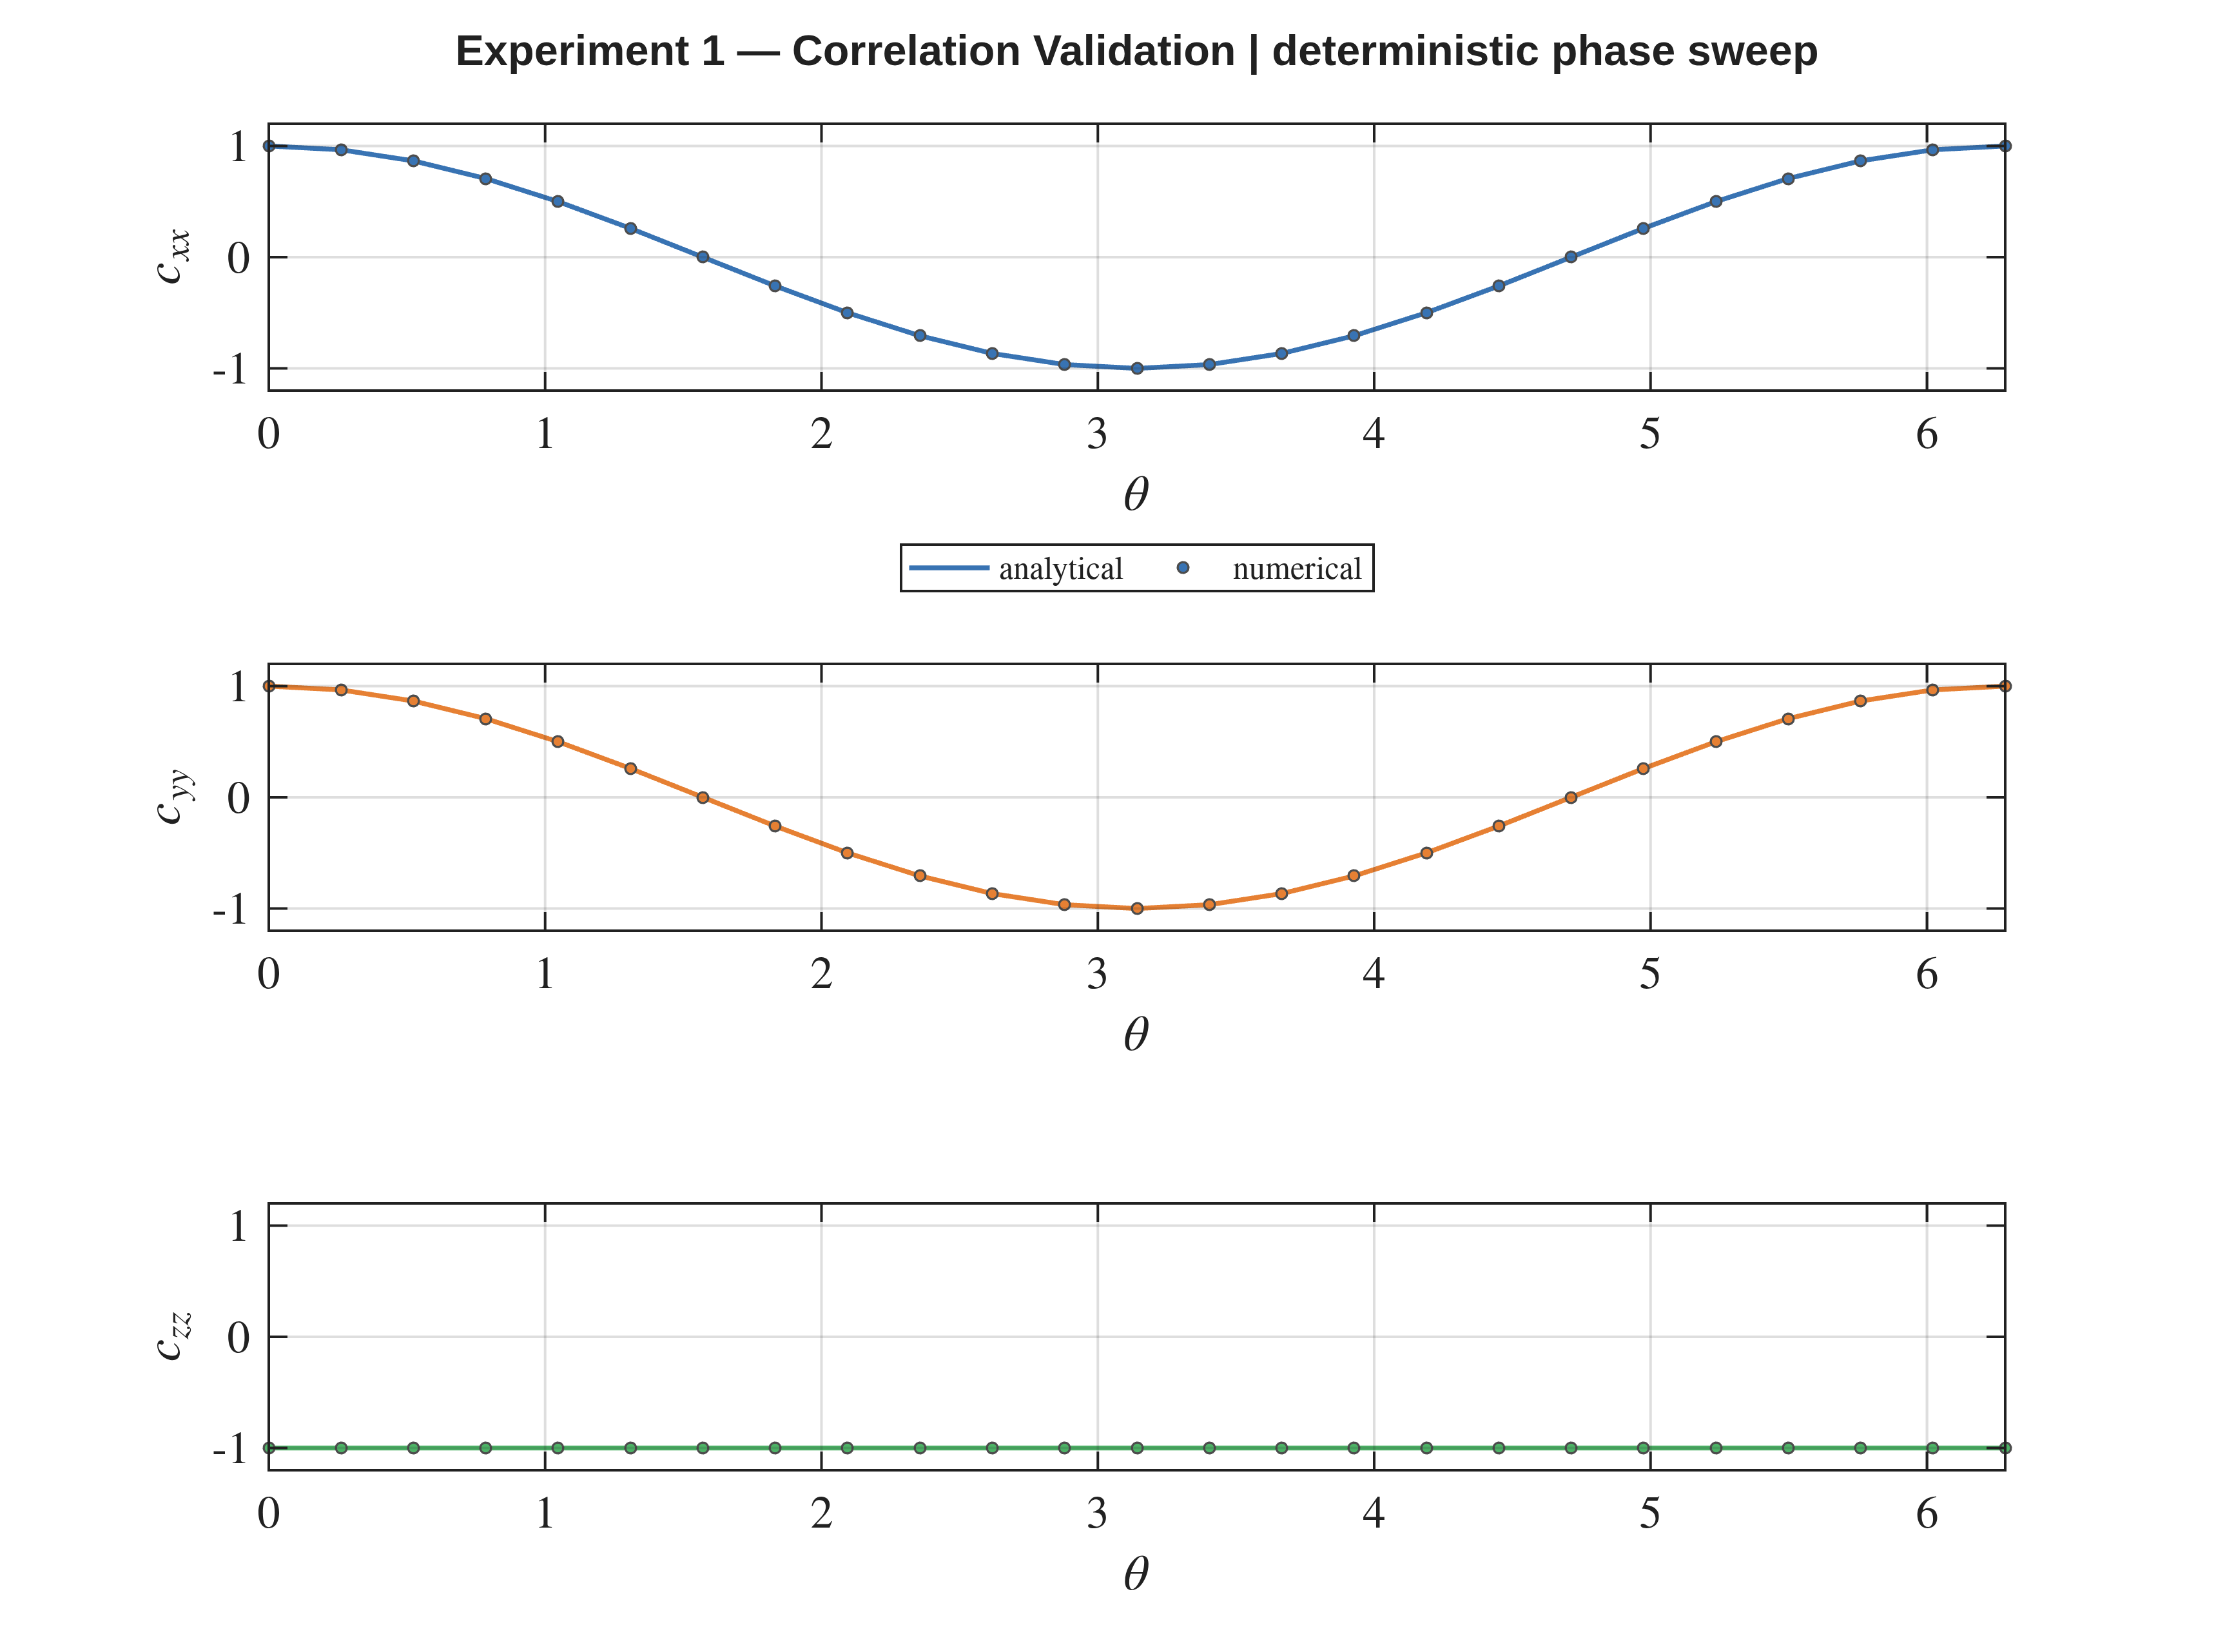
\includegraphics[width=0.75\linewidth]{../Images/Experiment_1/experiment_1_correlations_validation.png}
    \caption{
    Numerical and analytical comparison for the correlation observables \(c_{xx}\), \(c_{yy}\), and \(c_{zz}\).
    The agreement validates the implementation of the reduced phase model.
    }
    \label{fig:experiment1_validation}
\end{figure}

\begin{figure}[htbp]
    \centering
    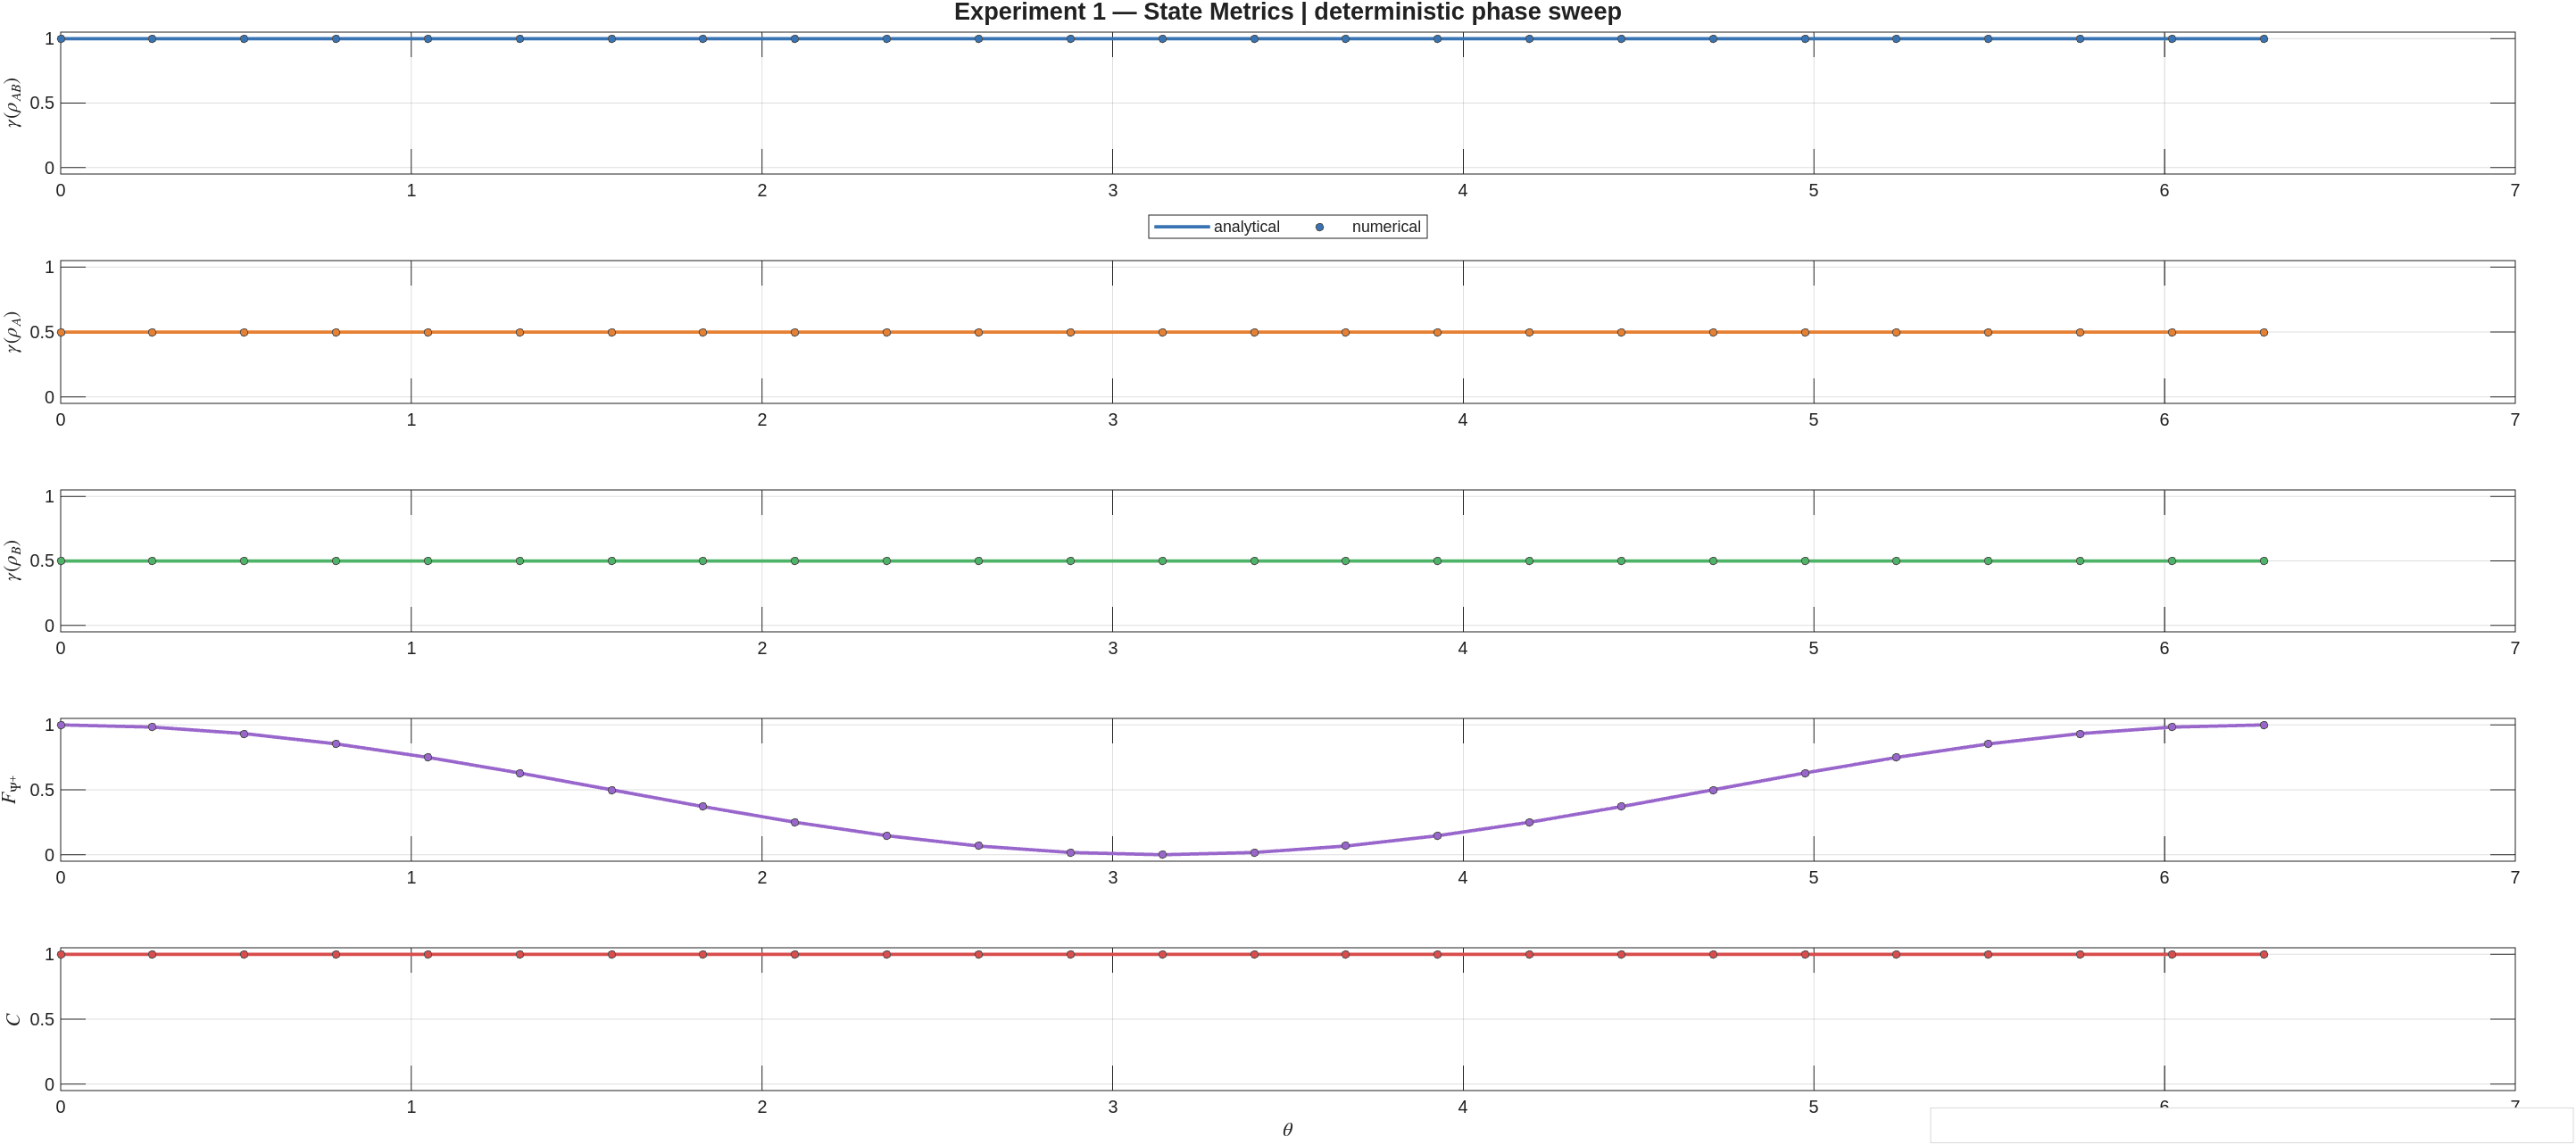
\includegraphics[width=0.75\linewidth]{../Images/Experiment_1/experiment_1_state_metrics.png}
    \caption{
    State-characterization quantities for the phase-evolved state.
    Global purity and concurrence remain constant, while fidelity varies with the relative phase \( \theta \).
    }
    \label{fig:experiment1_state_metrics}
\end{figure}

\begin{figure}[htbp]
    \centering
    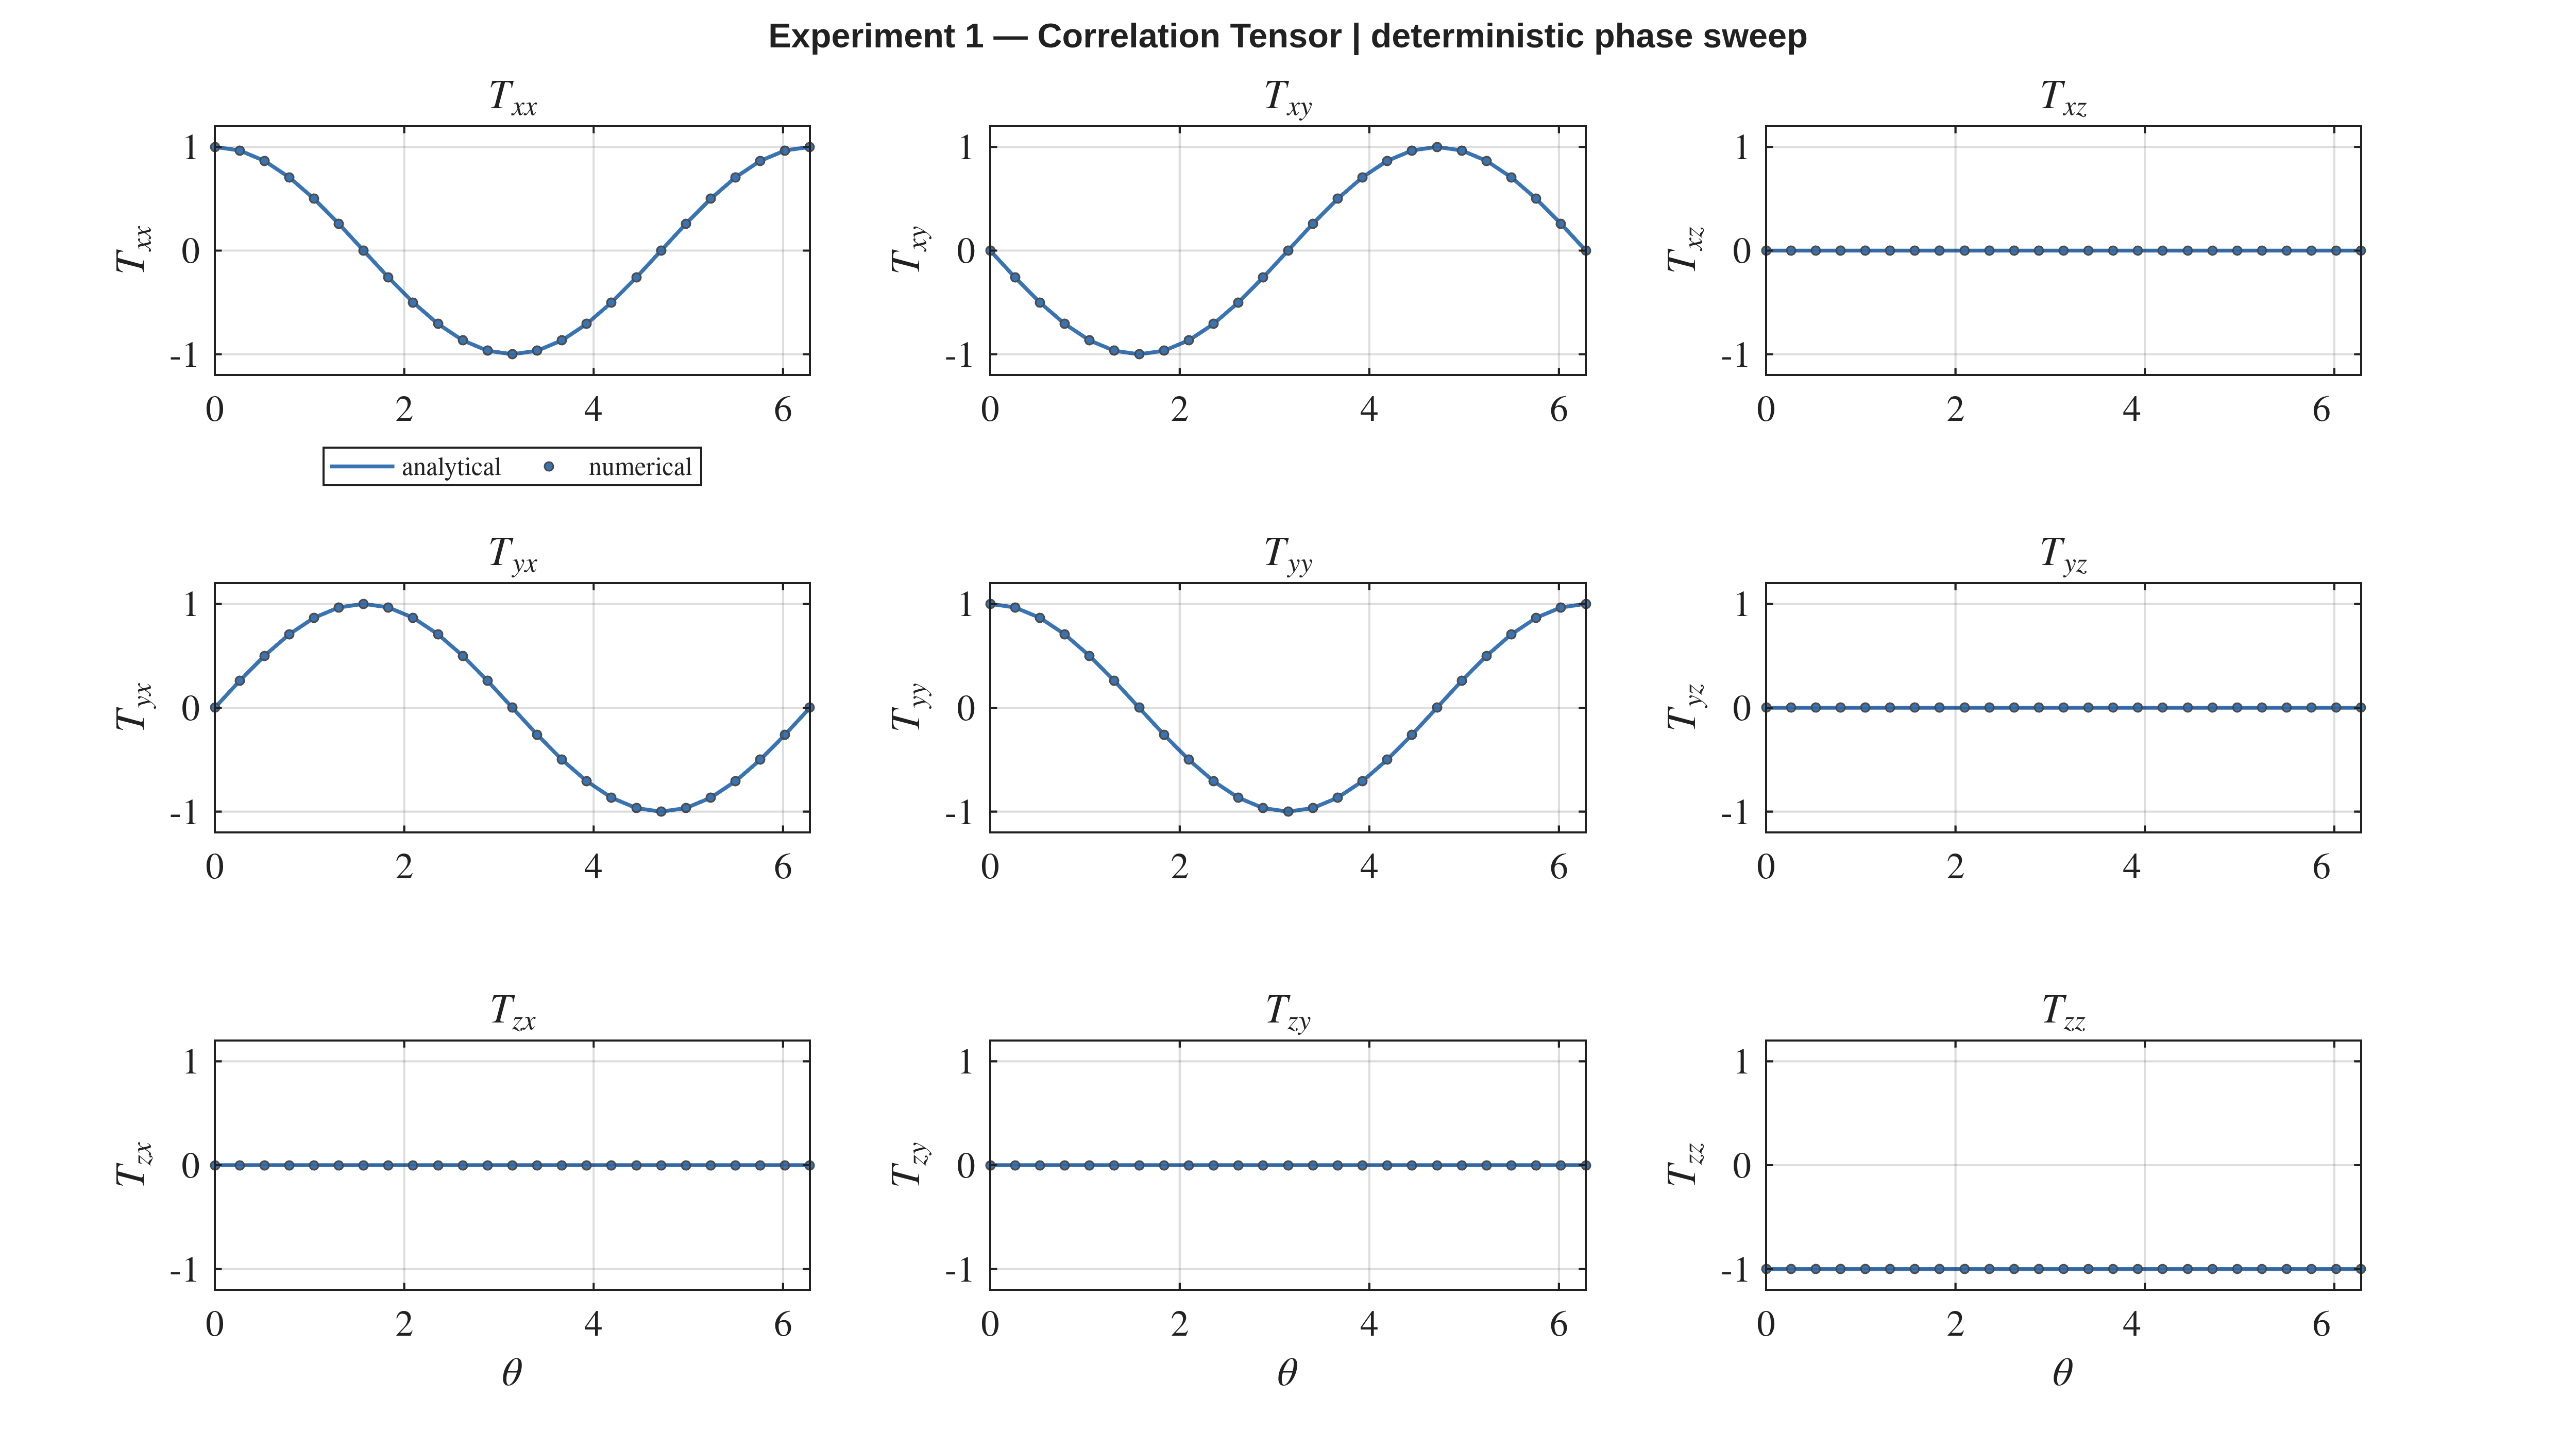
\includegraphics[width=0.85\linewidth]{../Images/Experiment_1/experiment_1_correlation_tensor.png}
    \caption{
    Full correlation tensor \(T_{ij}(\theta)\) for the phase-evolved state.
    The off-diagonal components \(T_{xy}\) and \(T_{yx}\) reveal the rotation of the correlation structure in the transverse plane.
    }
    \label{fig:experiment1_tensor}
\end{figure}

The numerical results confirm that the full correlation tensor takes the form
\[
T(\theta) =
\begin{pmatrix}
\cos\theta & -\sin\theta & 0\\
\sin\theta & \cos\theta & 0\\
0 & 0 & -1
\end{pmatrix}.
\]

This representation shows that the reduced phase model induces a rotation of the correlation structure in the \(x\)--\(y\) plane. In particular, the non-zero off-diagonal components
\[
T_{xy} = -\sin\theta,
\qquad
T_{yx} = \sin\theta
\]
encode the coupling between orthogonal measurement bases.

Therefore, the phase parameter \( \theta \) can be interpreted as a rotation angle of the correlation tensor around the \(z\)-axis in Bloch space. This structure is not visible when considering only the diagonal observables, but becomes explicit in the full tensor representation.

%--------------------------------------------------------
% Discussion
%--------------------------------------------------------

\subsubsection{Discussion}

The numerical results are in full agreement with the analytical predictions:
\begin{itemize}
\item \(c_{xx}\) and \(c_{yy}\) follow the expected cosine dependence;
\item \(c_{zz}\) remains constant at \(-1\);
\item the global purity remains equal to \(\gamma(\rho_{AB})=1\);
\item the reduced purities remain equal to \(\gamma(\rho_A)=\gamma(\rho_B)=1/2\);
\item the fidelity follows \(F_{\Psi^+}=(1+\cos\theta)/2\);
\item the concurrence remains constant at \(C=1\).
\end{itemize}

These results confirm that the fiber acts as an effective relative phase shifter. While the global state remains pure and maximally entangled, both the observable correlations and the fidelity with respect to a fixed Bell reference vary continuously with the phase.

A key observation is that fidelity and concurrence exhibit fundamentally different behaviors. Fidelity depends explicitly on \( \theta \), reflecting the overlap with a fixed reference state, whereas concurrence remains invariant. This confirms that fidelity does not provide a direct measure of entanglement.

Therefore, although phase evolution modifies observable correlations and the apparent similarity to a chosen Bell state, it does not alter the underlying entanglement structure.

%--------------------------------------------------------
% Physical Interpretation
%--------------------------------------------------------

\subsubsection{Physical Interpretation}

The results obtained in this experiment admit a direct physical interpretation in terms of fiber-induced birefringence. In optical fibers, the horizontal and vertical polarization components generally propagate with different effective refractive indices, leading to a relative phase accumulation.

After compensation of global polarization rotations, the dominant residual effect is a differential phase shift between the two polarization modes. In the quantum description, this corresponds to a local unitary transformation equivalent to a rotation around the \(Z\)-axis of the Bloch sphere.

As a consequence, the initial Bell state evolves into a phase-dependent superposition while preserving its entangled nature. The invariance of concurrence reflects the fact that no information is lost during propagation and the global state remains pure.

At the same time, the phase dependence of the transverse correlations \(c_{xx}\) and \(c_{yy}\) demonstrates that measurable quantities are sensitive to this relative phase. The parameter \( \theta \) is therefore the key variable controlling observable correlations in the absence of noise.

This experiment establishes the minimal physical model of fiber propagation: a deterministic unitary transformation that modifies observable correlations without degrading entanglement.


%========================================================
% Subsection 5.2 — Experiment 2: Random Phase Ensemble
%========================================================

\newpage

\subsection{Experiment 2: Random Phase Ensemble}

%--------------------------------------------------------
% Objective
%--------------------------------------------------------

\subsubsection{Objective}

The second experiment extends the deterministic phase model by introducing random phase realizations \( \theta_k \), modeling stochastic birefringence effects in realistic optical fibers.

Instead of a single pure state, the system is described by an ensemble
\[
\{ |\psi(\theta_k)\rangle \}_{k=1}^{N},
\]
and by the corresponding averaged density operator.

The objective is to characterize how ensemble averaging modifies global coherence, correlation observables, purity, fidelity, and entanglement.

%--------------------------------------------------------
% Model
%--------------------------------------------------------

\subsubsection{Model}

Each realization is given by
\[
|\psi(\theta_k)\rangle
=
\frac{1}{\sqrt{2}}
\left(
|01\rangle + e^{i\theta_k}|10\rangle
\right),
\]
and the ensemble state is
\[
\rho_{\mathrm{ensemble}}
=
\frac{1}{N}
\sum_{k=1}^{N}
|\psi(\theta_k)\rangle\langle \psi(\theta_k)|.
\]

%--------------------------------------------------------
% Analytical Predictions
%--------------------------------------------------------

\subsubsection{Analytical Predictions}

Introducing the ensemble coherence parameter
\[
\mu = \langle e^{i\theta} \rangle
=
\langle \cos\theta \rangle + i \langle \sin\theta \rangle,
\]
the ensemble-averaged correlations are
\[
c_{xx} = \mathrm{Re}(\mu),\qquad
c_{yy} = \mathrm{Re}(\mu),\qquad
c_{zz} = -1.
\]

The global purity is
\[
\gamma(\rho_{\mathrm{ensemble}})
=
\frac{1 + |\mu|^2}{2}.
\]

The reduced states remain maximally mixed:
\[
\rho_A = \rho_B = \frac{I}{2}, 
\qquad
\gamma(\rho_A)=\gamma(\rho_B)=\frac{1}{2}.
\]

The fidelity and concurrence are
\[
F_{\Psi^+}
=
\frac{1 + \mathrm{Re}(\mu)}{2},
\qquad
C(\rho_{\mathrm{ensemble}}) = |\mu|.
\]

%--------------------------------------------------------
% Numerical Results
%--------------------------------------------------------

\subsubsection{Numerical Results}

Three representative phase distributions are considered:
\begin{itemize}
\item constant phase,
\item uniform distribution,
\item Gaussian distribution.
\end{itemize}

Each case is summarized in a single figure combining:
\begin{itemize}
\item sampled phase statistics,
\item pure-state correlation trend,
\item ensemble correlations,
\item purity, fidelity, and concurrence.
\end{itemize}

\begin{figure}[htbp]
\centering
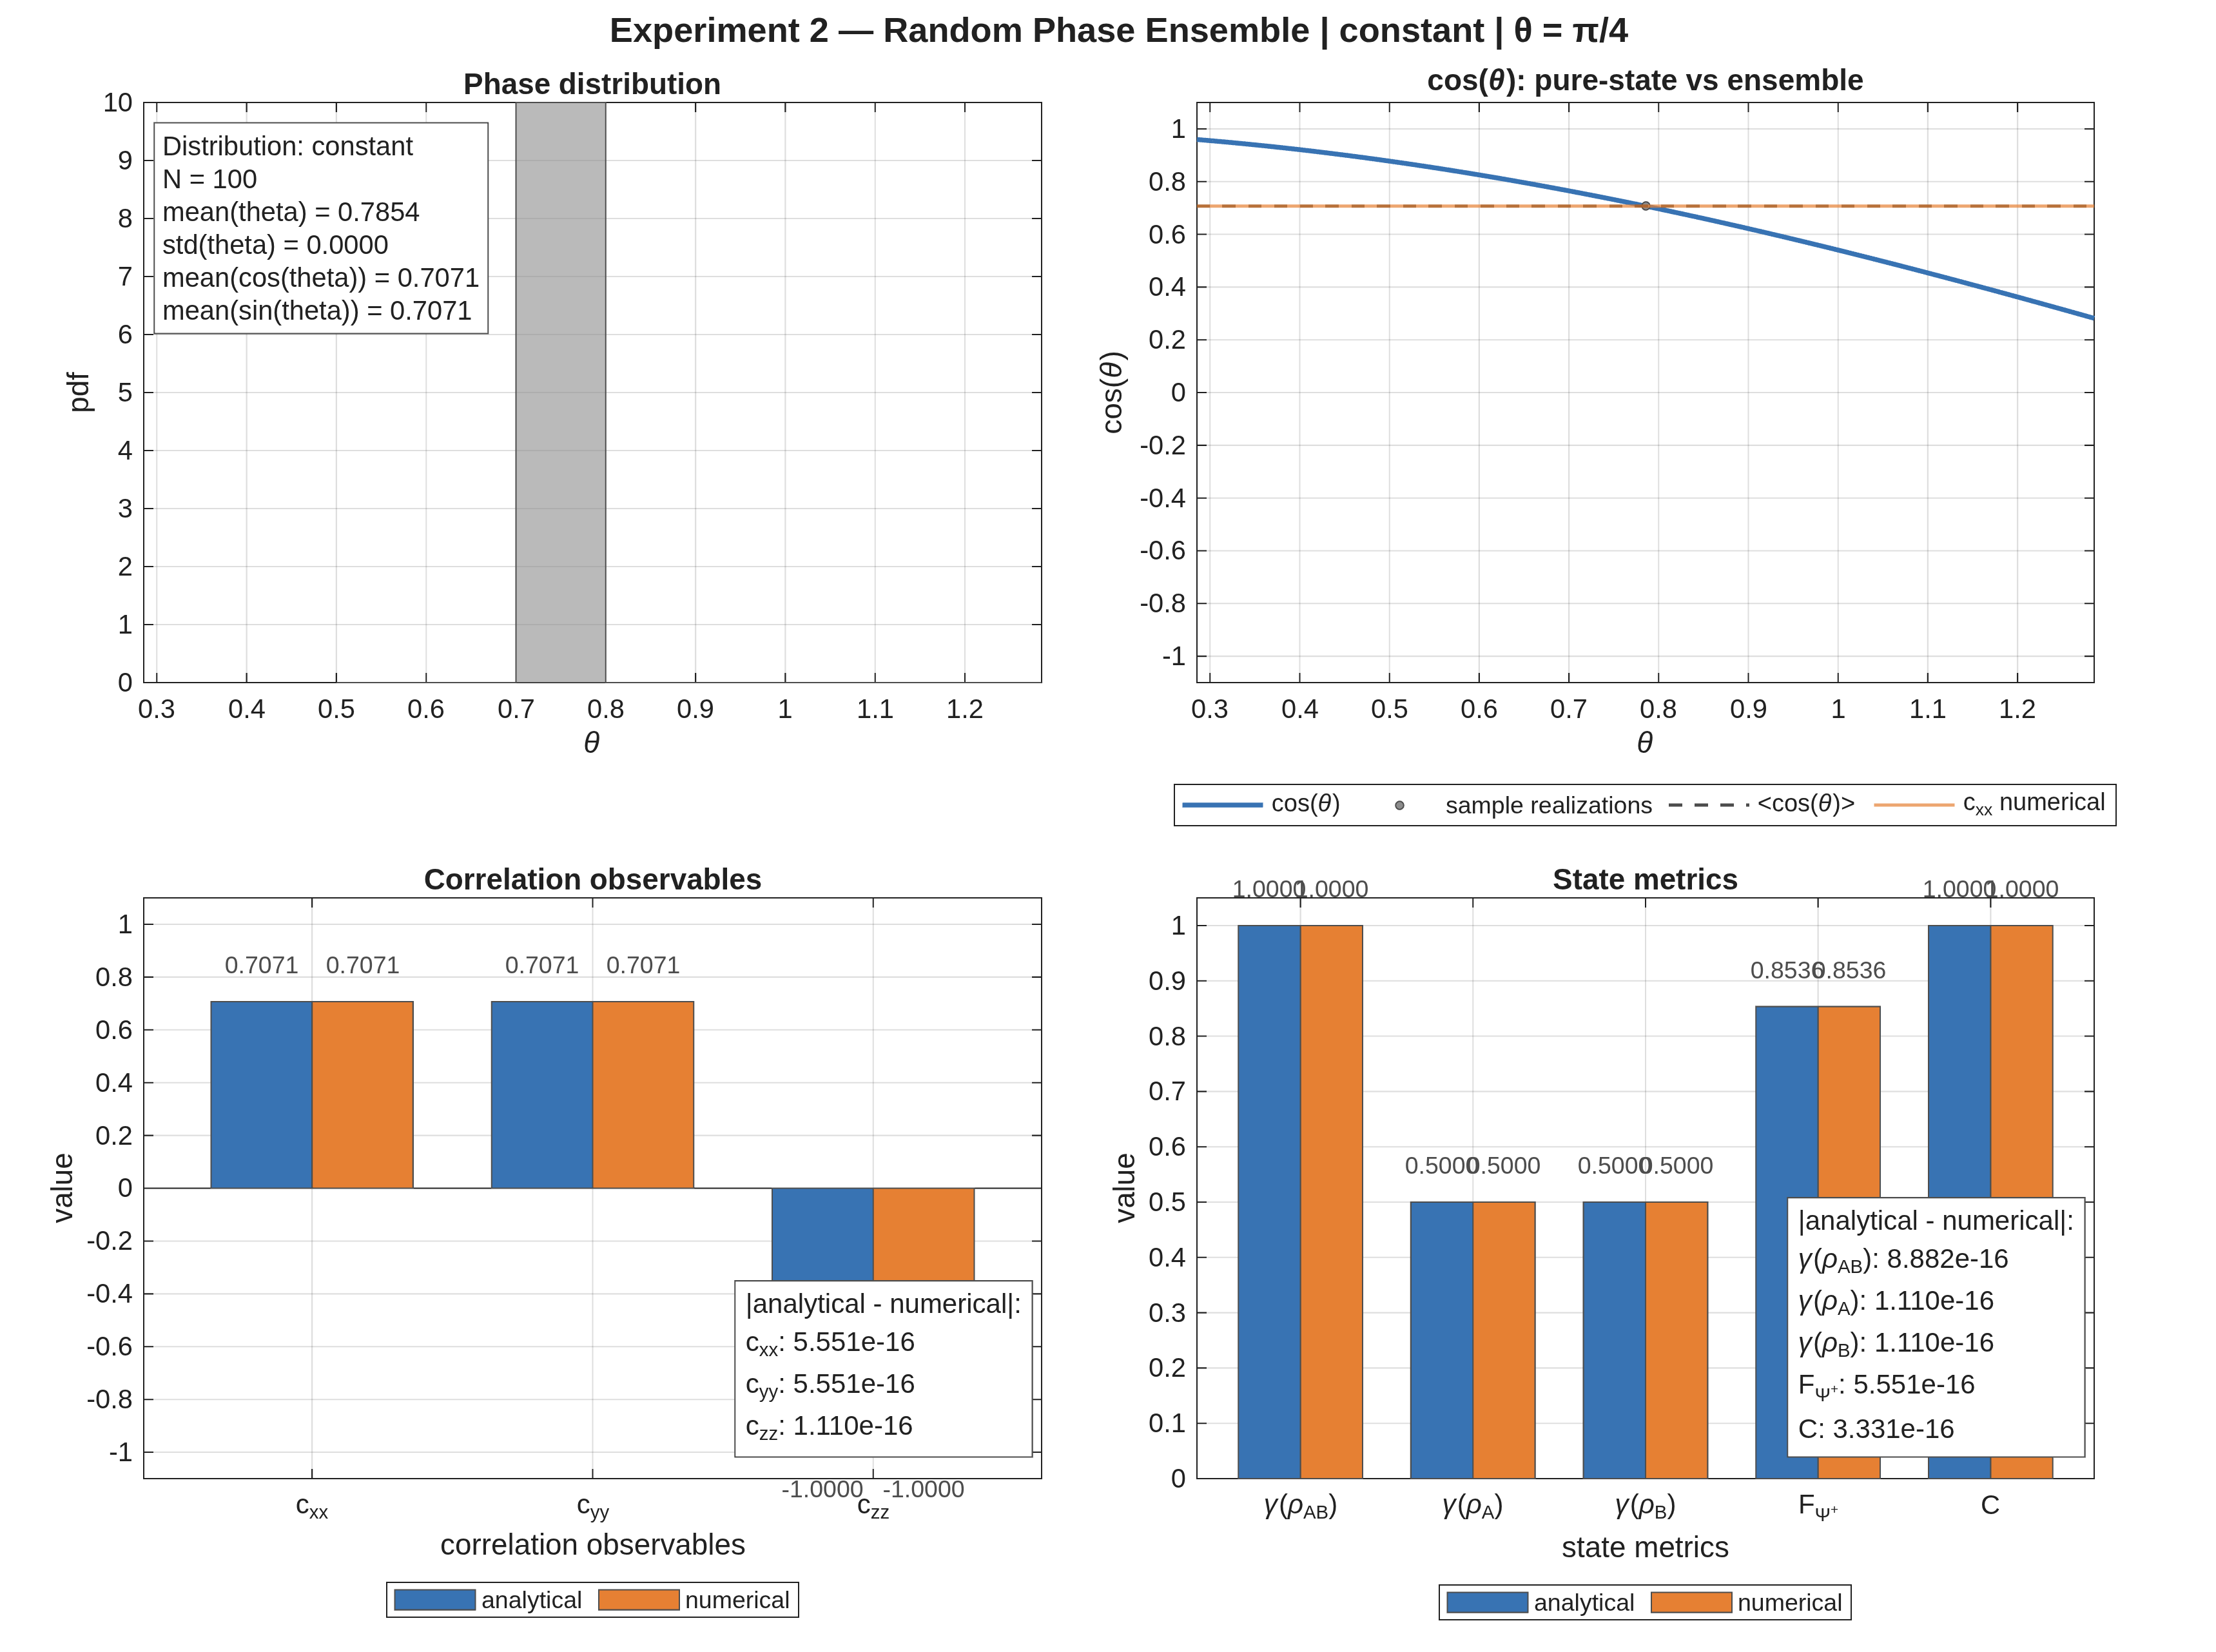
\includegraphics[width=0.9\linewidth]{../Images/Experiment_2/experiment_2_summary_constant_distribution.png}
\caption{
Constant phase distribution: the ensemble reduces to a deterministic realization and concurrence remains maximal.
}
\label{fig:experiment2_constant}
\end{figure}

\begin{figure}[htbp]
\centering
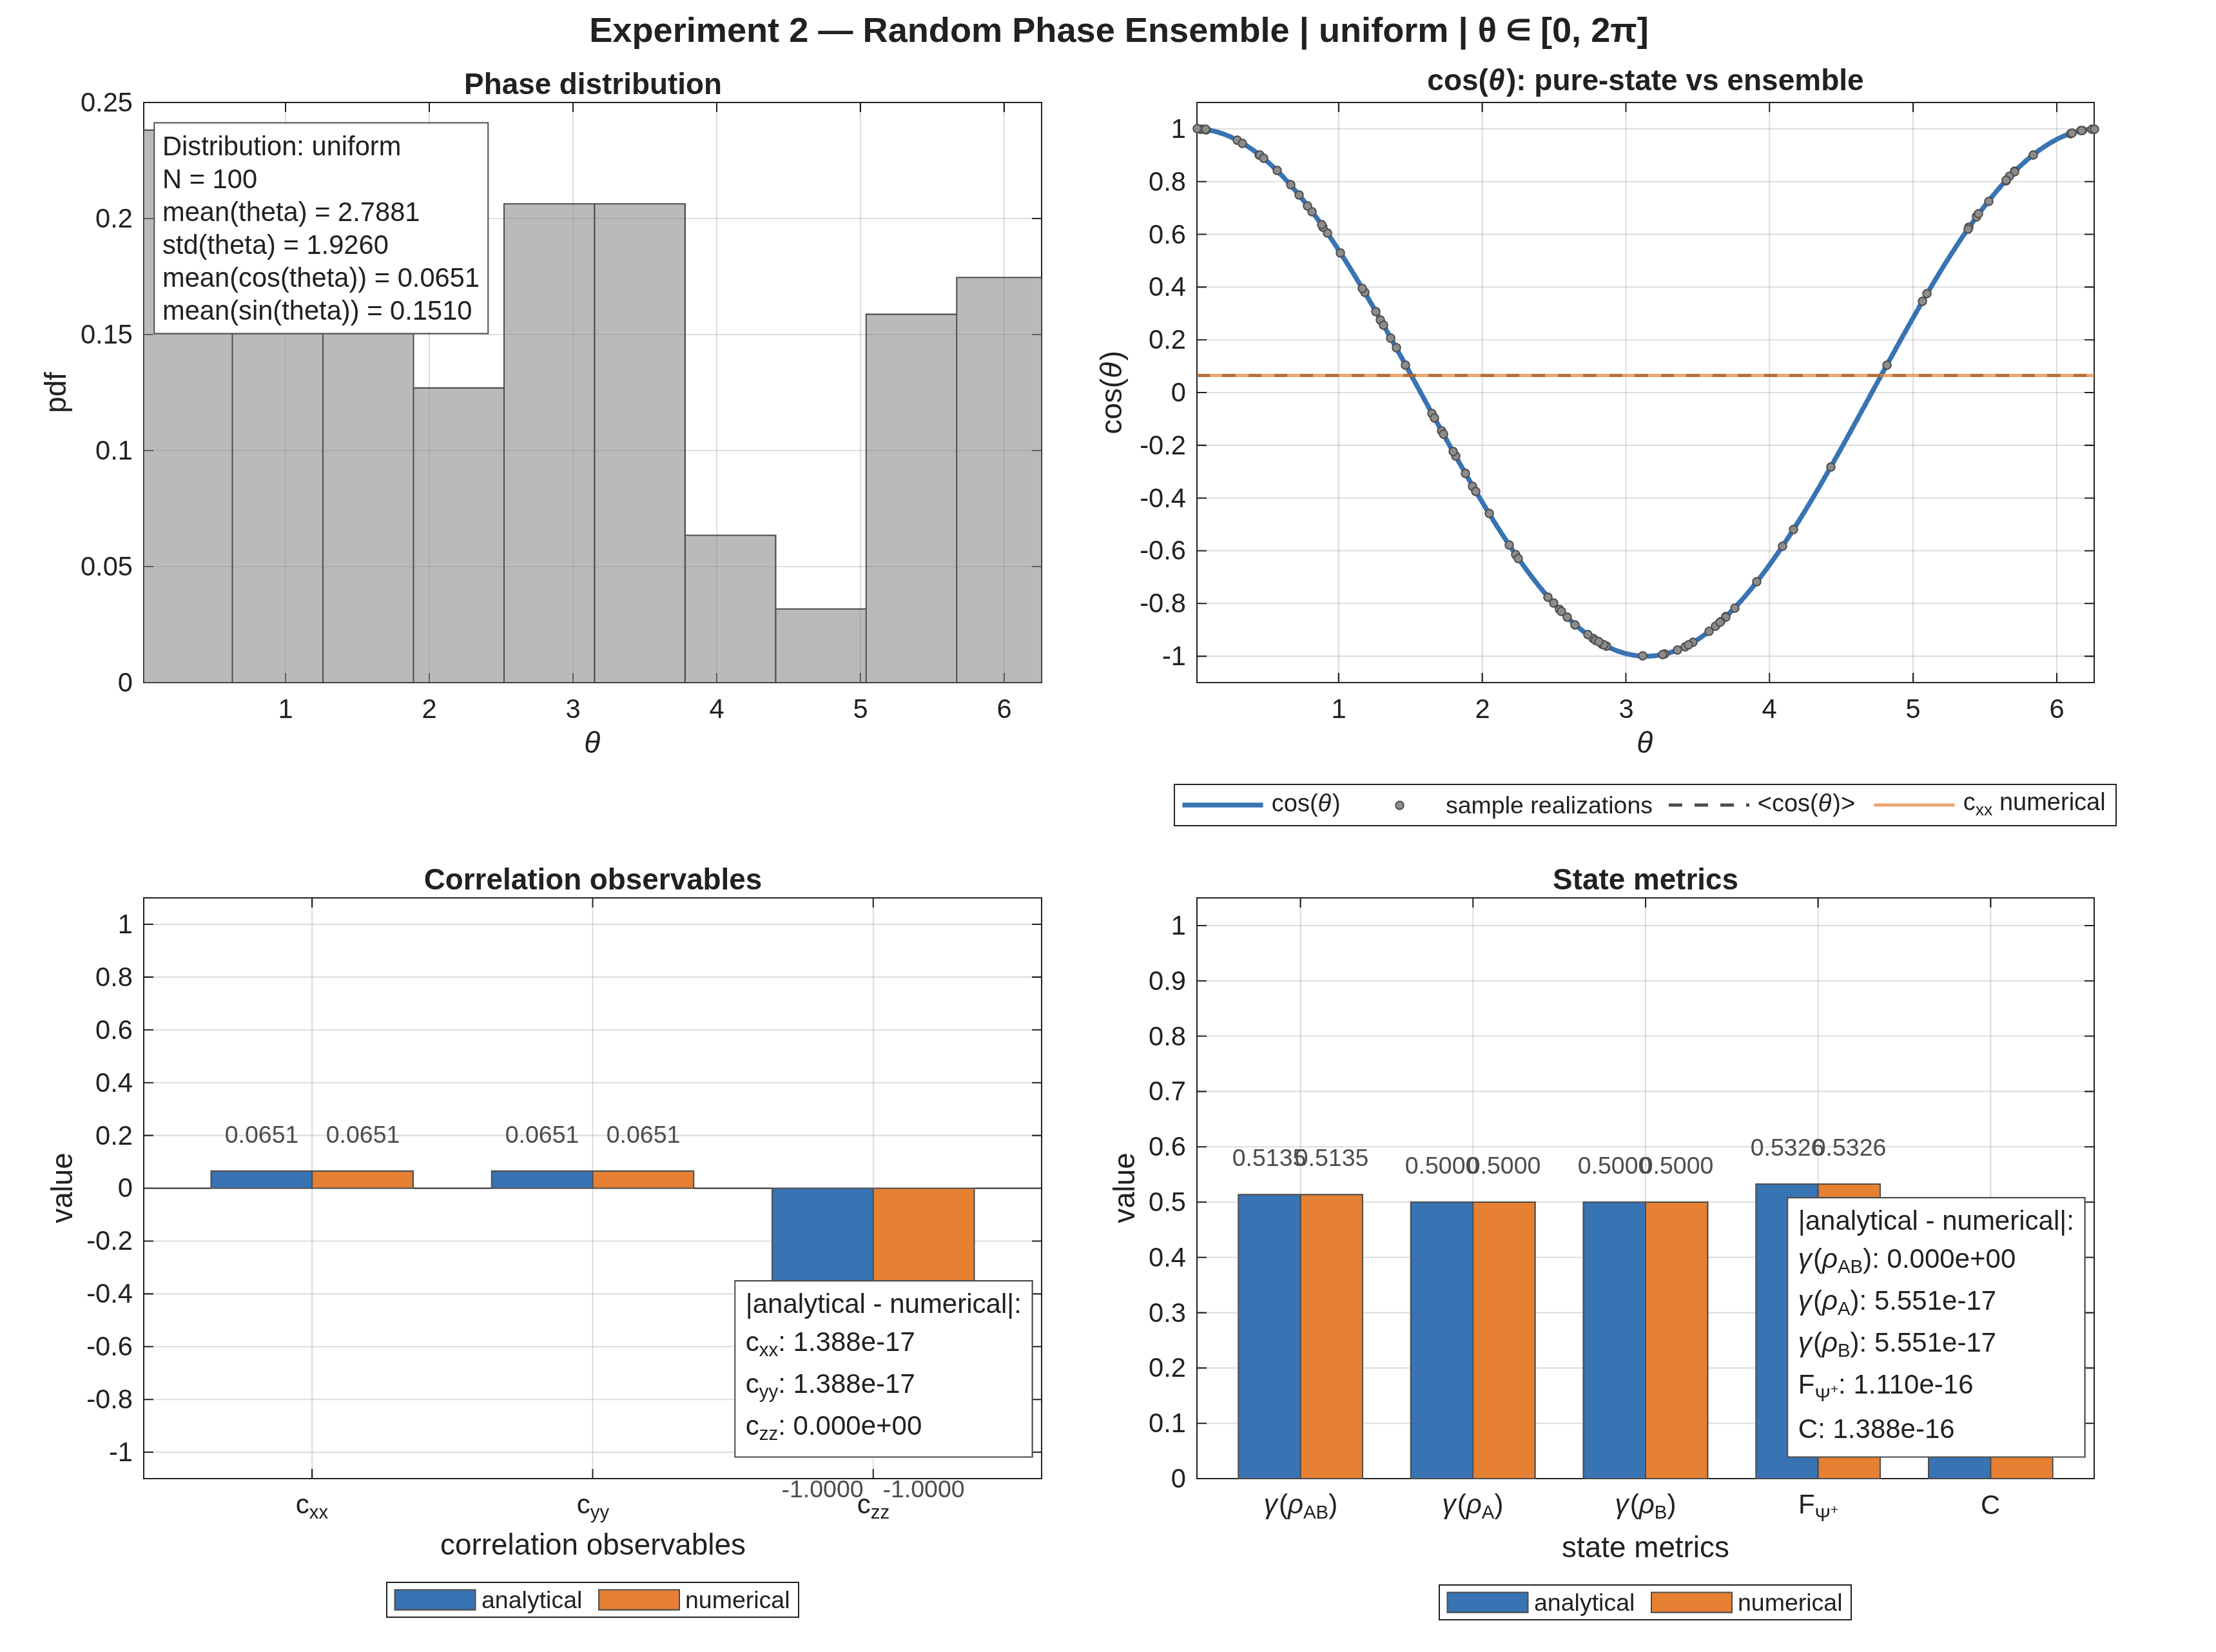
\includegraphics[width=0.9\linewidth]{../Images/Experiment_2/experiment_2_summary_uniform_distribution.png}
\caption{
Uniform phase distribution: transverse correlations vanish, fidelity decreases, and concurrence tends to zero.
}
\label{fig:experiment2_uniform}
\end{figure}

\begin{figure}[htbp]
\centering
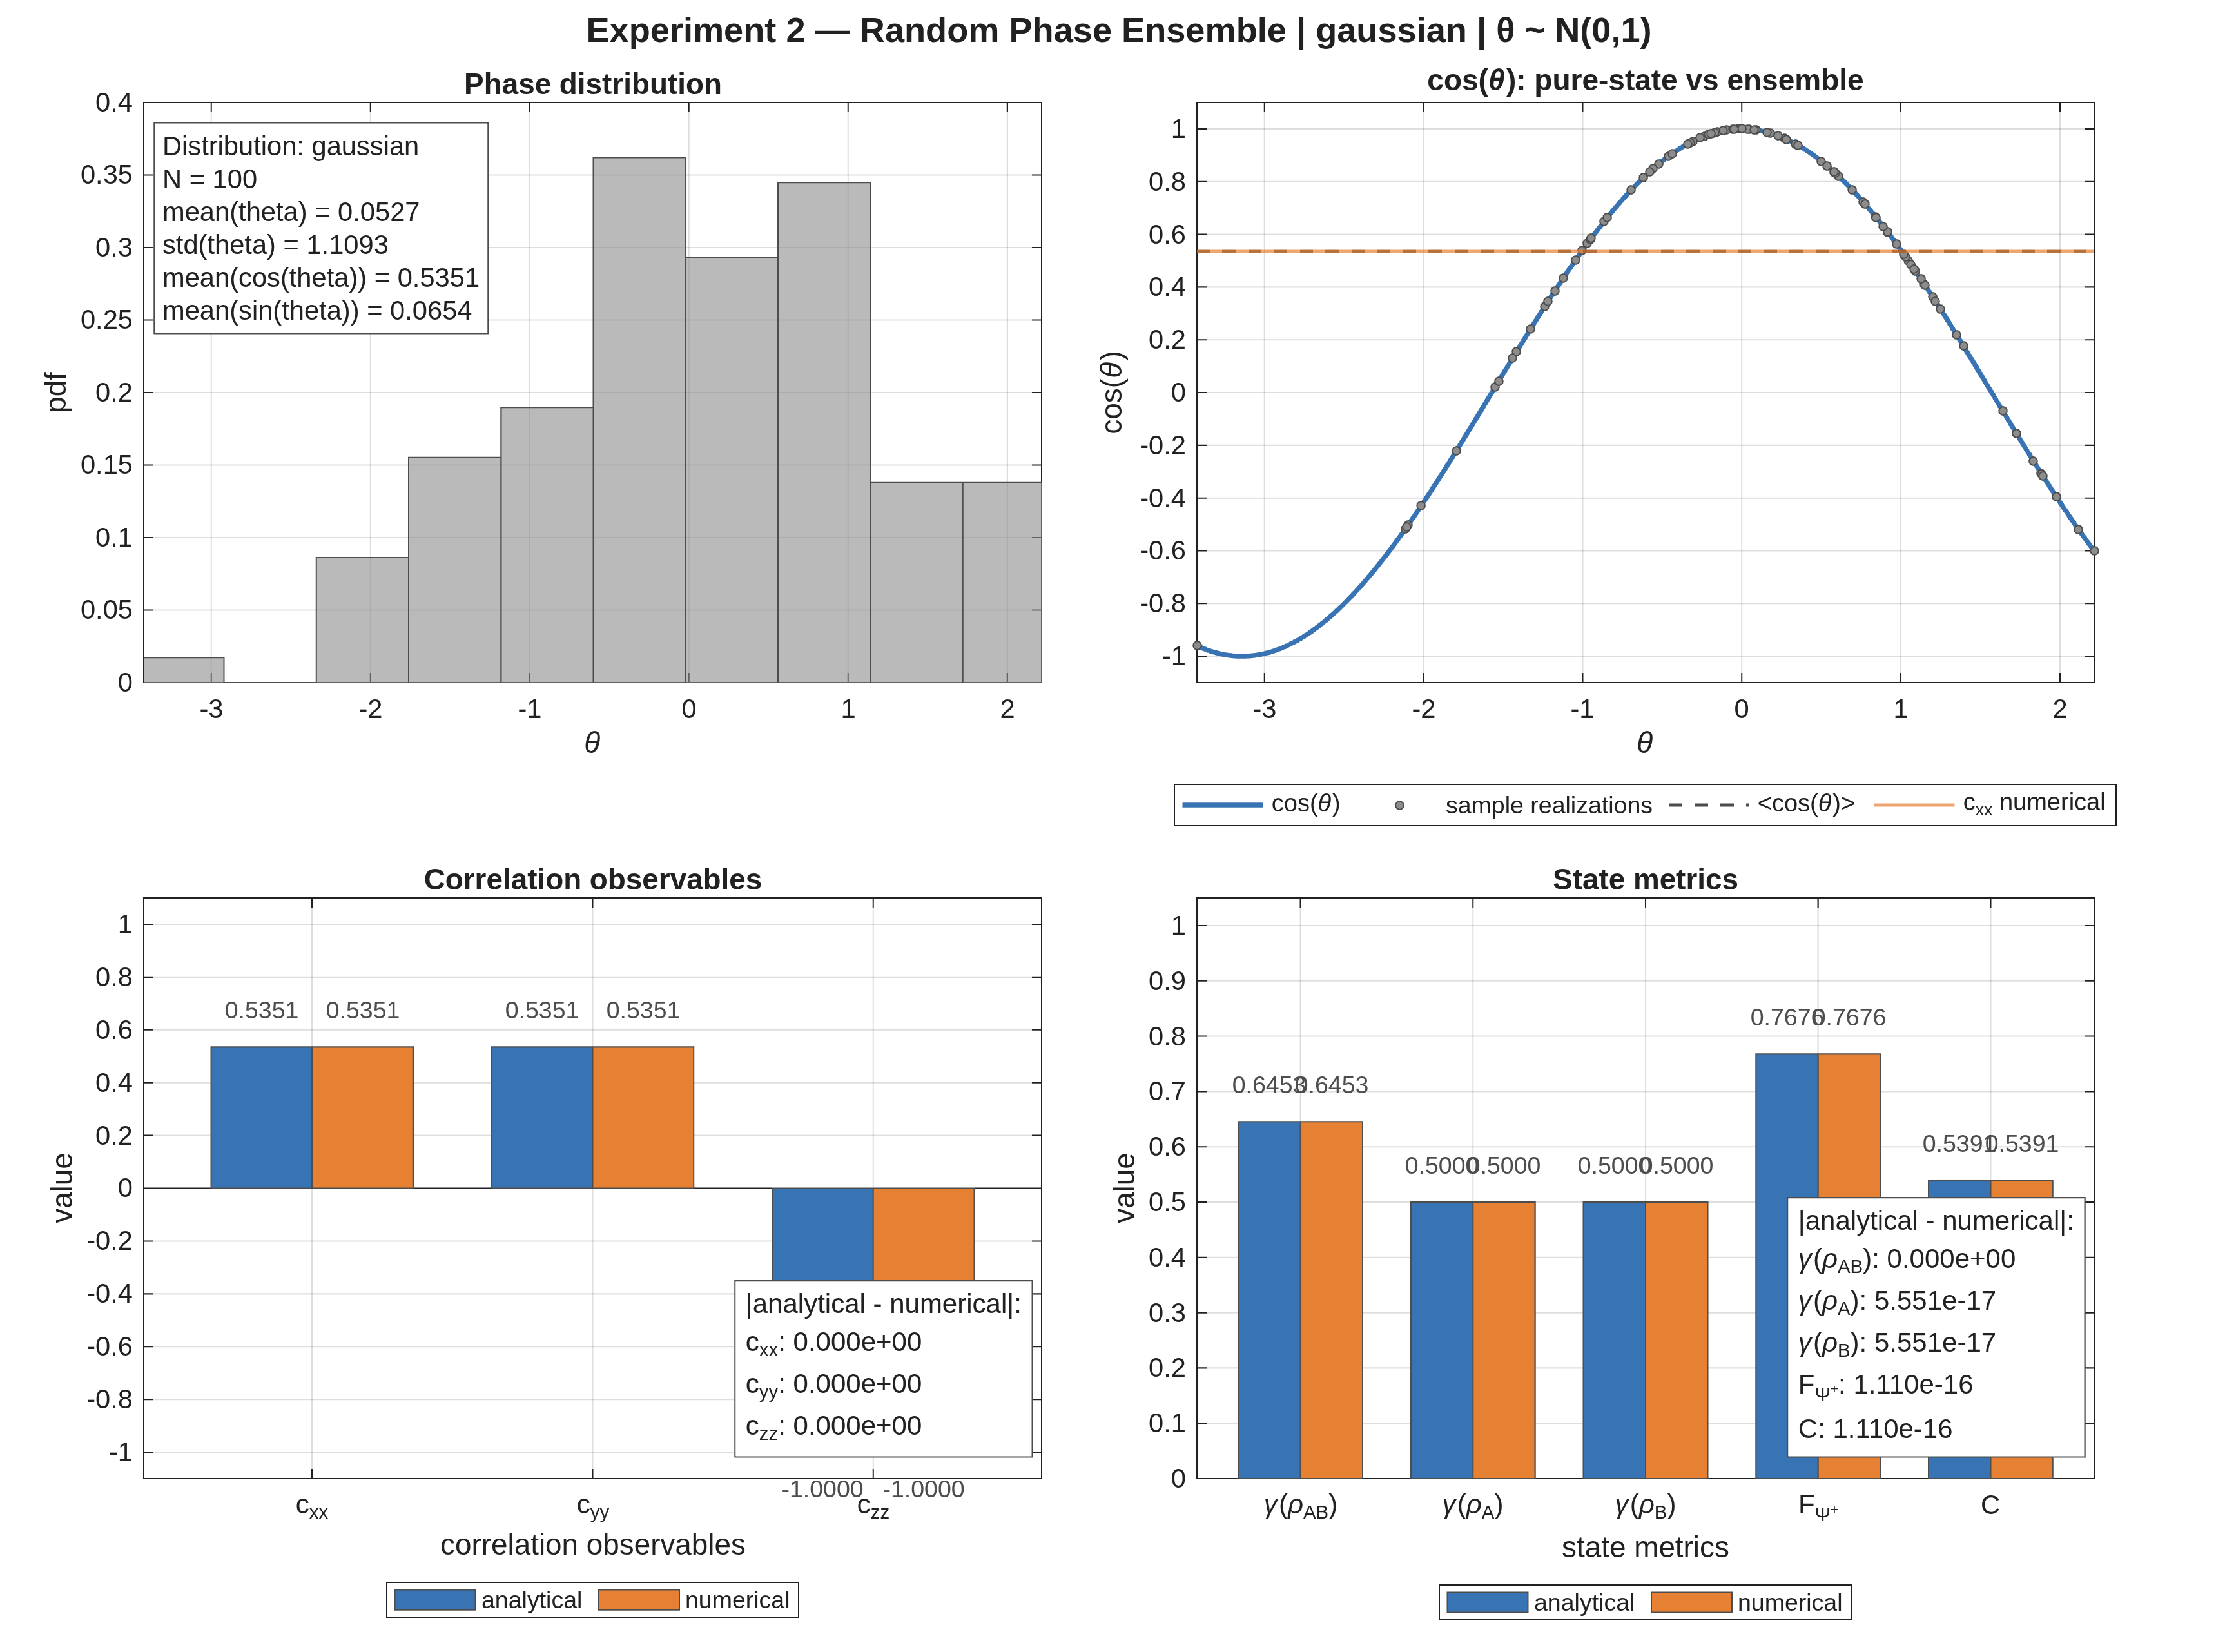
\includegraphics[width=0.9\linewidth]{../Images/Experiment_2/experiment_2_summary_gaussian_distribution.png}
\caption{
Gaussian phase distribution: partial coherence leads to intermediate values of purity and concurrence.
}
\label{fig:experiment2_gaussian}
\end{figure}

\begin{figure}[htbp]
\centering

\begin{subfigure}{0.32\linewidth}
    \centering
    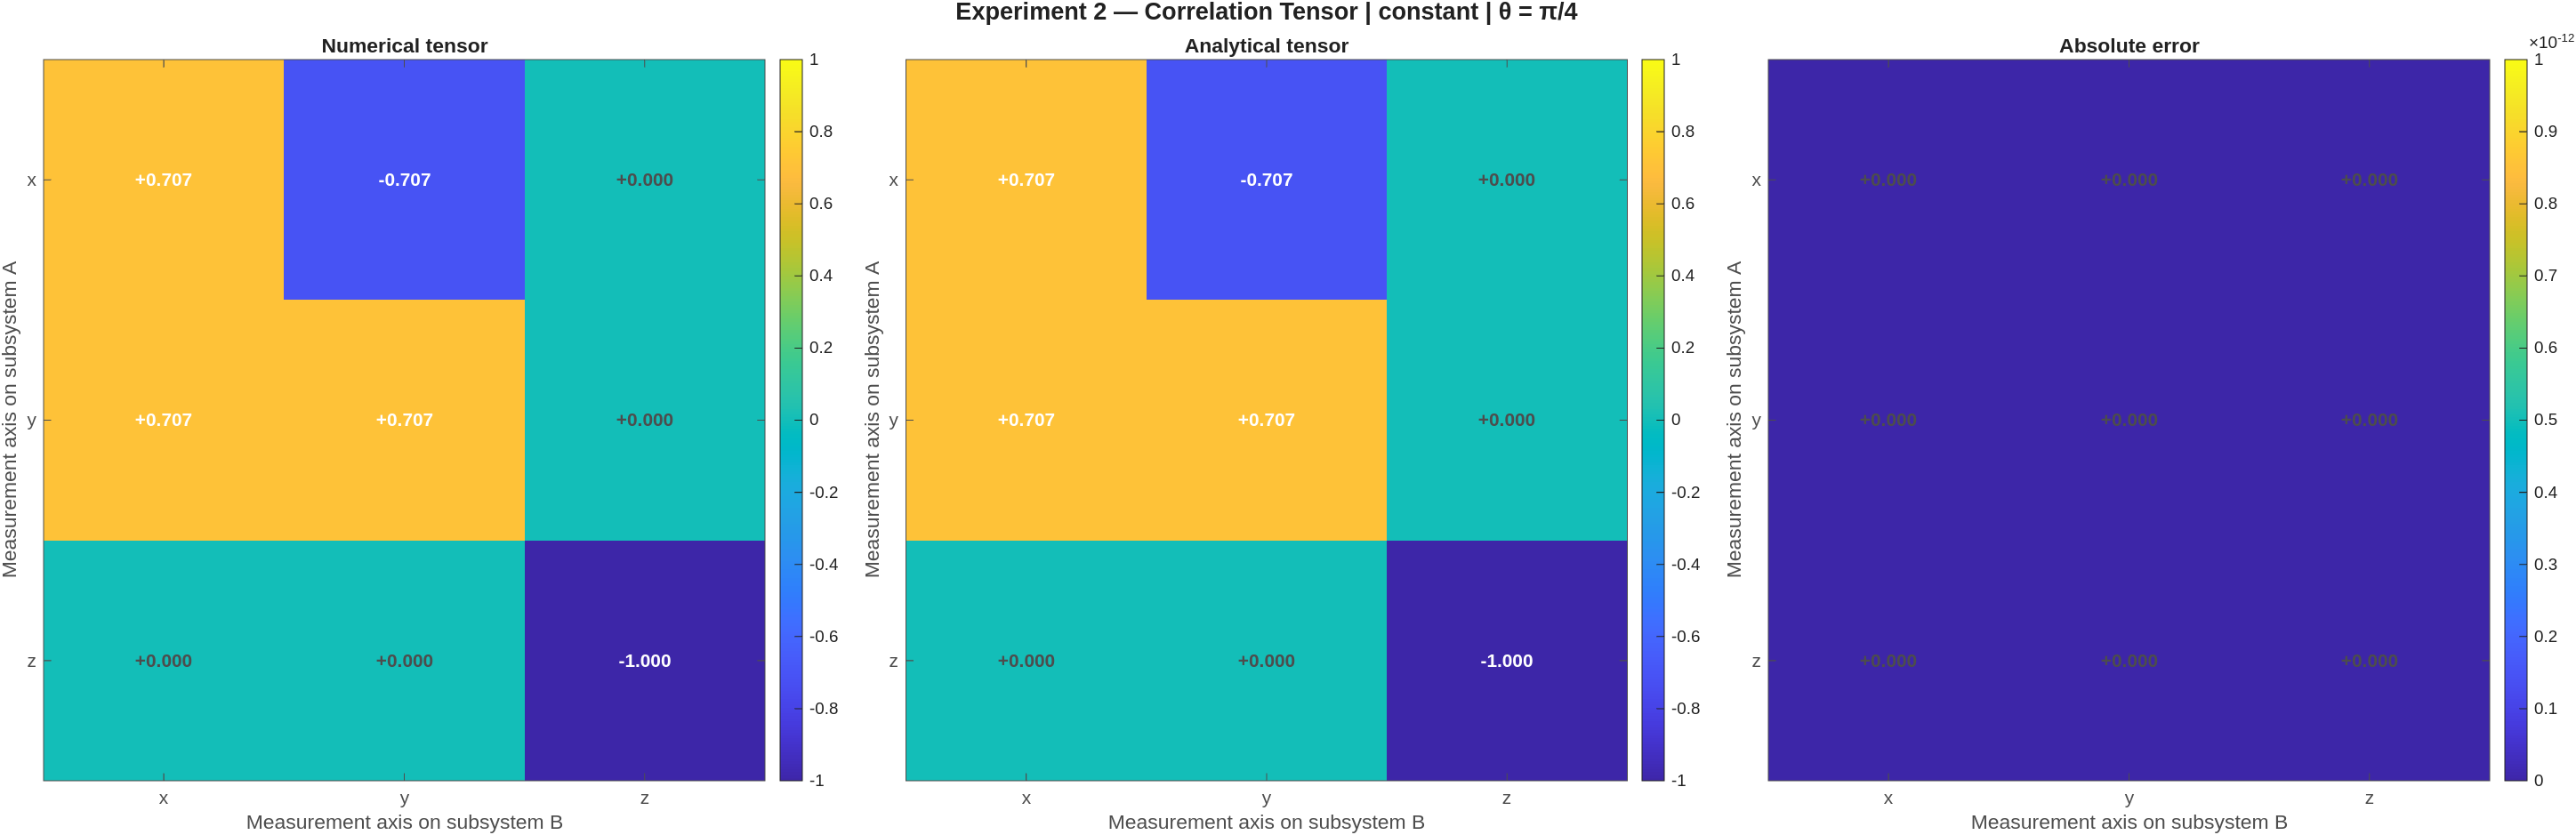
\includegraphics[width=\linewidth]{../Images/Experiment_2/experiment_2_correlation_tensor_constant.png}
    \caption{Constant phase}
\end{subfigure}
\hfill
\begin{subfigure}{0.32\linewidth}
    \centering
    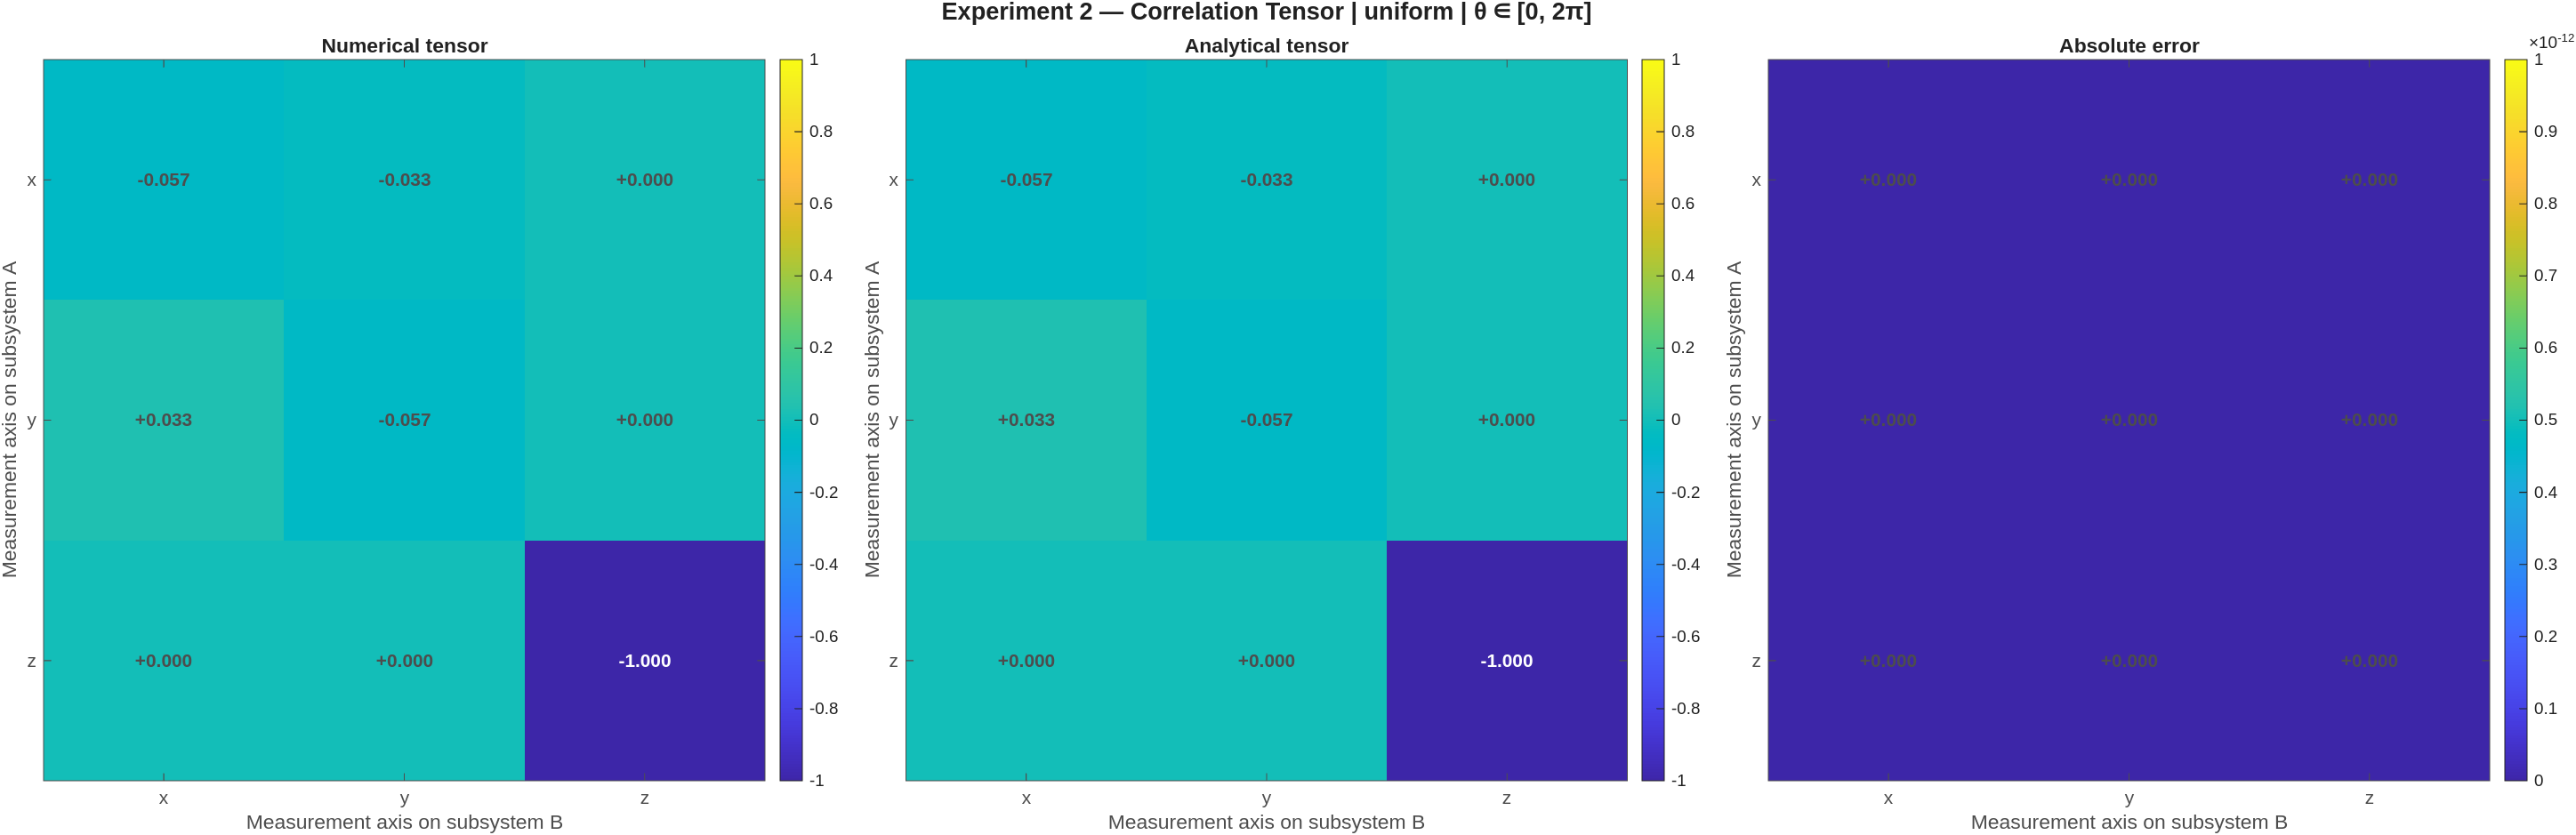
\includegraphics[width=\linewidth]{../Images/Experiment_2/experiment_2_correlation_tensor_uniform.png}
    \caption{Uniform distribution}
\end{subfigure}
\hfill
\begin{subfigure}{0.32\linewidth}
    \centering
    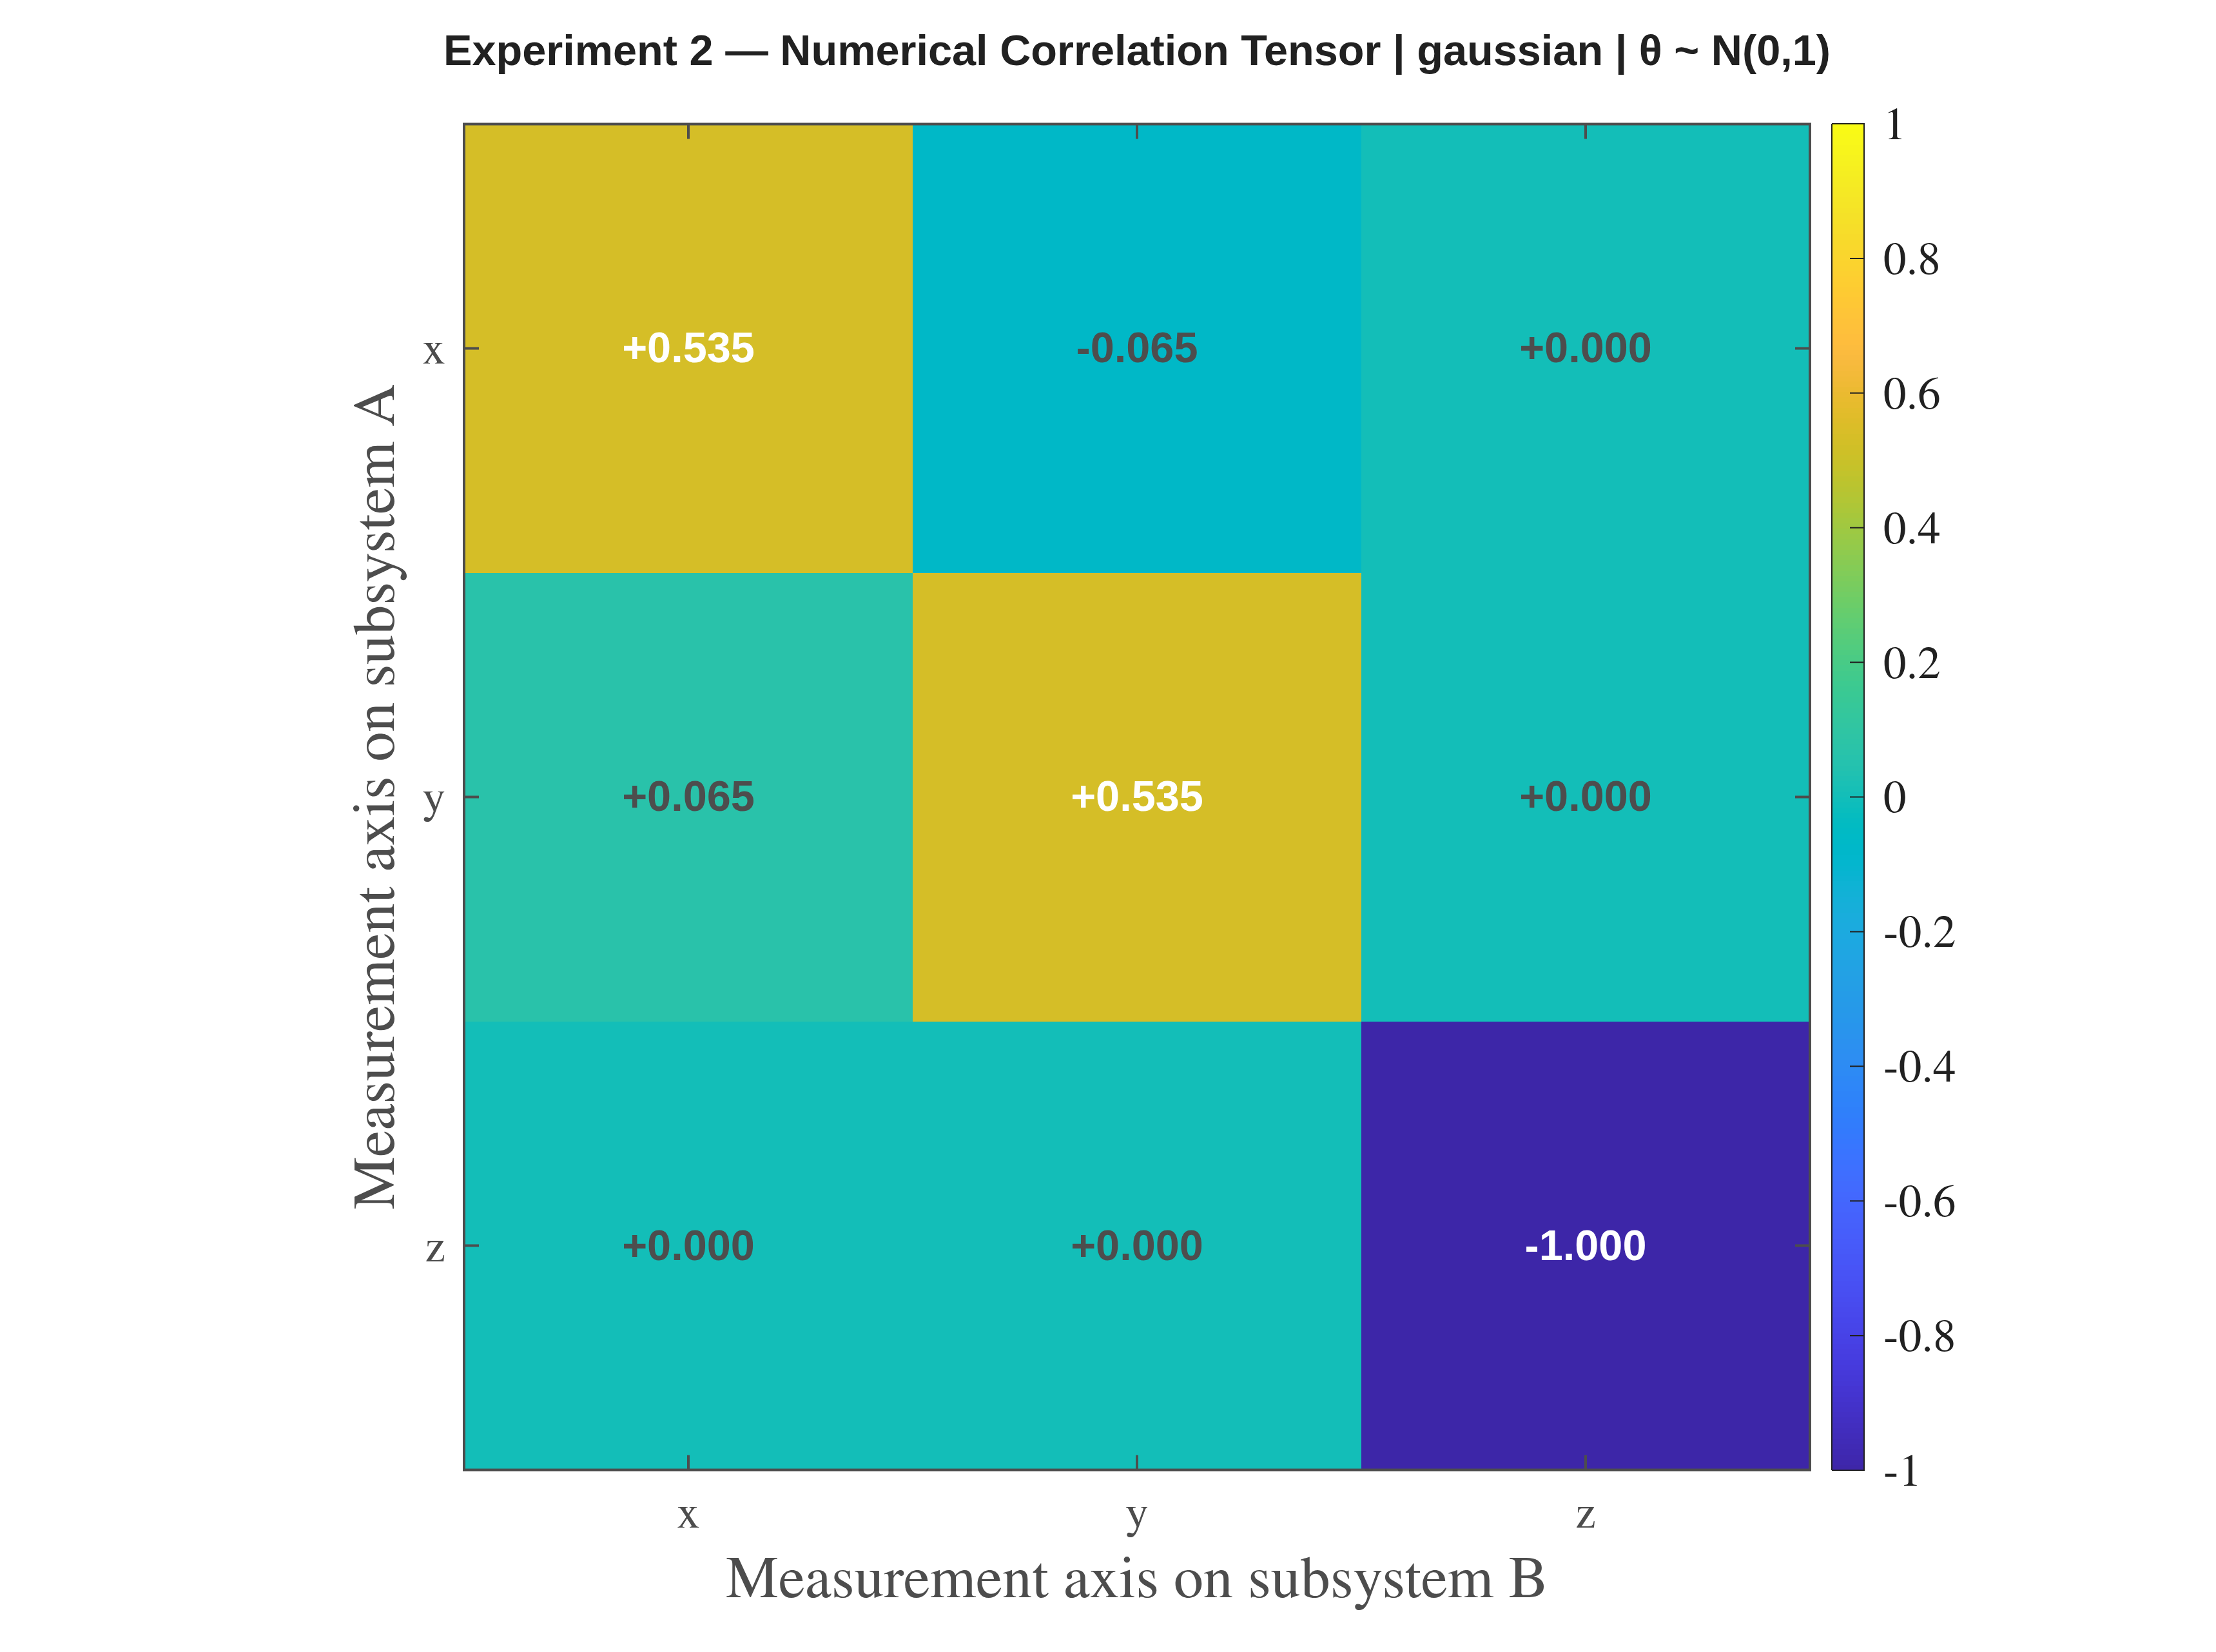
\includegraphics[width=\linewidth]{../Images/Experiment_2/experiment_2_correlation_tensor_gaussian.png}
    \caption{Gaussian distribution}
\end{subfigure}

\caption{
Correlation tensor snapshots for Experiment 2 under different phase distributions.
Random phase averaging suppresses transverse coherence, leading to a reduction of the off-diagonal components, while the longitudinal correlation \( T_{zz} = -1 \) remains invariant.
For statistical ensembles, the transverse components converge to their analytical expectation values as the number of samples \( N \) increases.
In contrast, tensor entries that are analytically zero are identically zero in the simulation, reflecting the exact symmetry of the model.
}
\label{fig:experiment2_tensor_snapshots}
\end{figure}

%--------------------------------------------------------
% Discussion
%--------------------------------------------------------

\subsubsection{Discussion}

The results show a transition from deterministic to ensemble behavior:
\begin{itemize}
\item constant phase reproduces Experiment~1,
\item distributed phases reduce transverse correlations,
\item broad distributions lead to \( |\mu| \to 0 \) and vanishing coherence.
\end{itemize}

Accordingly:
\begin{itemize}
\item global purity decreases from \(1\),
\item reduced purities remain fixed at \(1/2\),
\item fidelity decreases,
\item concurrence decreases from \(1\) to \(0\).
\end{itemize}

Unlike the deterministic case, the reduction of fidelity is here associated with a genuine loss of entanglement, as quantified by concurrence.

%--------------------------------------------------------
% Physical Interpretation
%--------------------------------------------------------

\subsubsection{Physical Interpretation}

Each realization remains a pure maximally entangled state, while mixedness arises from averaging over unresolved phase fluctuations.

The coherence parameter \( \mu = \langle e^{i\theta} \rangle \) provides a unified description: its real part determines observable correlations and fidelity, while its magnitude controls entanglement.

Thus, ensemble averaging leads to a progressive loss of coherence and entanglement, capturing the transition from ideal unitary evolution to realistic noisy propagation in optical fibers.


%========================================================
% Subsection 5.3 — Experiment 3: Depolarizing Channel
%========================================================

\newpage

\subsection{Experiment 3: Depolarizing Channel}

%--------------------------------------------------------
% Objective
%--------------------------------------------------------

\subsubsection{Objective}

This experiment studies the degradation of a maximally entangled Bell state under an effective two-qubit depolarizing channel. Unlike previous experiments based on unitary or ensemble-averaged evolution, the present model introduces a genuinely non-unitary transformation at the level of the density operator.

The objectives are:
\begin{itemize}
\item to validate the depolarizing channel introduced in Section~3.9;
\item to quantify its effect on purity, fidelity, concurrence, correlations, and the correlation tensor;
\item to compare numerical results with analytical predictions over \(p \in [0,1]\).
\end{itemize}

%--------------------------------------------------------
% Model
%--------------------------------------------------------

\subsubsection{Model}

The input state is the Bell state
\[
|\Psi^+\rangle = \frac{|01\rangle + |10\rangle}{\sqrt{2}},
\qquad
\rho_0 = |\Psi^+\rangle\langle\Psi^+|.
\]

The depolarizing channel is defined as
\[
\rho(p) = (1-p)\rho_0 + \frac{p}{4}I_4,
\qquad p \in [0,1].
\]

This interpolates between
\[
\rho(0)=\rho_0,
\qquad
\rho(1)=\frac{I_4}{4}.
\]

%--------------------------------------------------------
% Analytical Predictions
%--------------------------------------------------------

\subsubsection{Analytical Predictions}

For this family of states:
\[
\gamma_{AB}(p)=1-\frac{3}{2}p+\frac{3}{4}p^2,
\qquad
\gamma_A=\gamma_B=\frac{1}{2},
\]
\[
F_{\Psi^+}(p)=1-\frac{3}{4}p,
\qquad
C(p)=\max\!\left(0,\,1-\frac{3}{2}p\right).
\]

The concurrence vanishes at
\[
p=\frac{2}{3},
\]
marking the transition to separability.

The action of the depolarizing channel on the correlation tensor is a uniform contraction of the Bell-state tensor:
\[
T(p) = (1-p)T_{\Psi^+}.
\]

Using
\[
T_{\Psi^+}
=
\begin{pmatrix}
1 & 0 & 0 \\
0 & 1 & 0 \\
0 & 0 & -1
\end{pmatrix},
\]
one obtains
\[
T(p)
=
\begin{pmatrix}
1-p & 0 & 0 \\
0 & 1-p & 0 \\
0 & 0 & -(1-p)
\end{pmatrix}.
\]

Therefore, the diagonal correlations are
\[
c_{xx}(p)=1-p,\qquad
c_{yy}(p)=1-p,\qquad
c_{zz}(p)=-(1-p).
\]

These expressions are consistent with the correlation-tensor formalism introduced in Section~3.5 and with the analytical derivation reported in Appendix~D.

%--------------------------------------------------------
% Numerical Results
%--------------------------------------------------------

\subsubsection{Numerical Results}

The parameter \(p\) is sampled over \([0,1]\), and all observables are computed and compared to analytical predictions.

The numerical results show agreement at machine precision for all quantities, confirming the correctness of the implementation. In particular, the maximum Frobenius-norm error of the correlation tensor is of order \(10^{-16}\), while the errors on purity, fidelity, concurrence, and diagonal correlations remain at numerical roundoff level.

\begin{figure}[htbp]
\centering
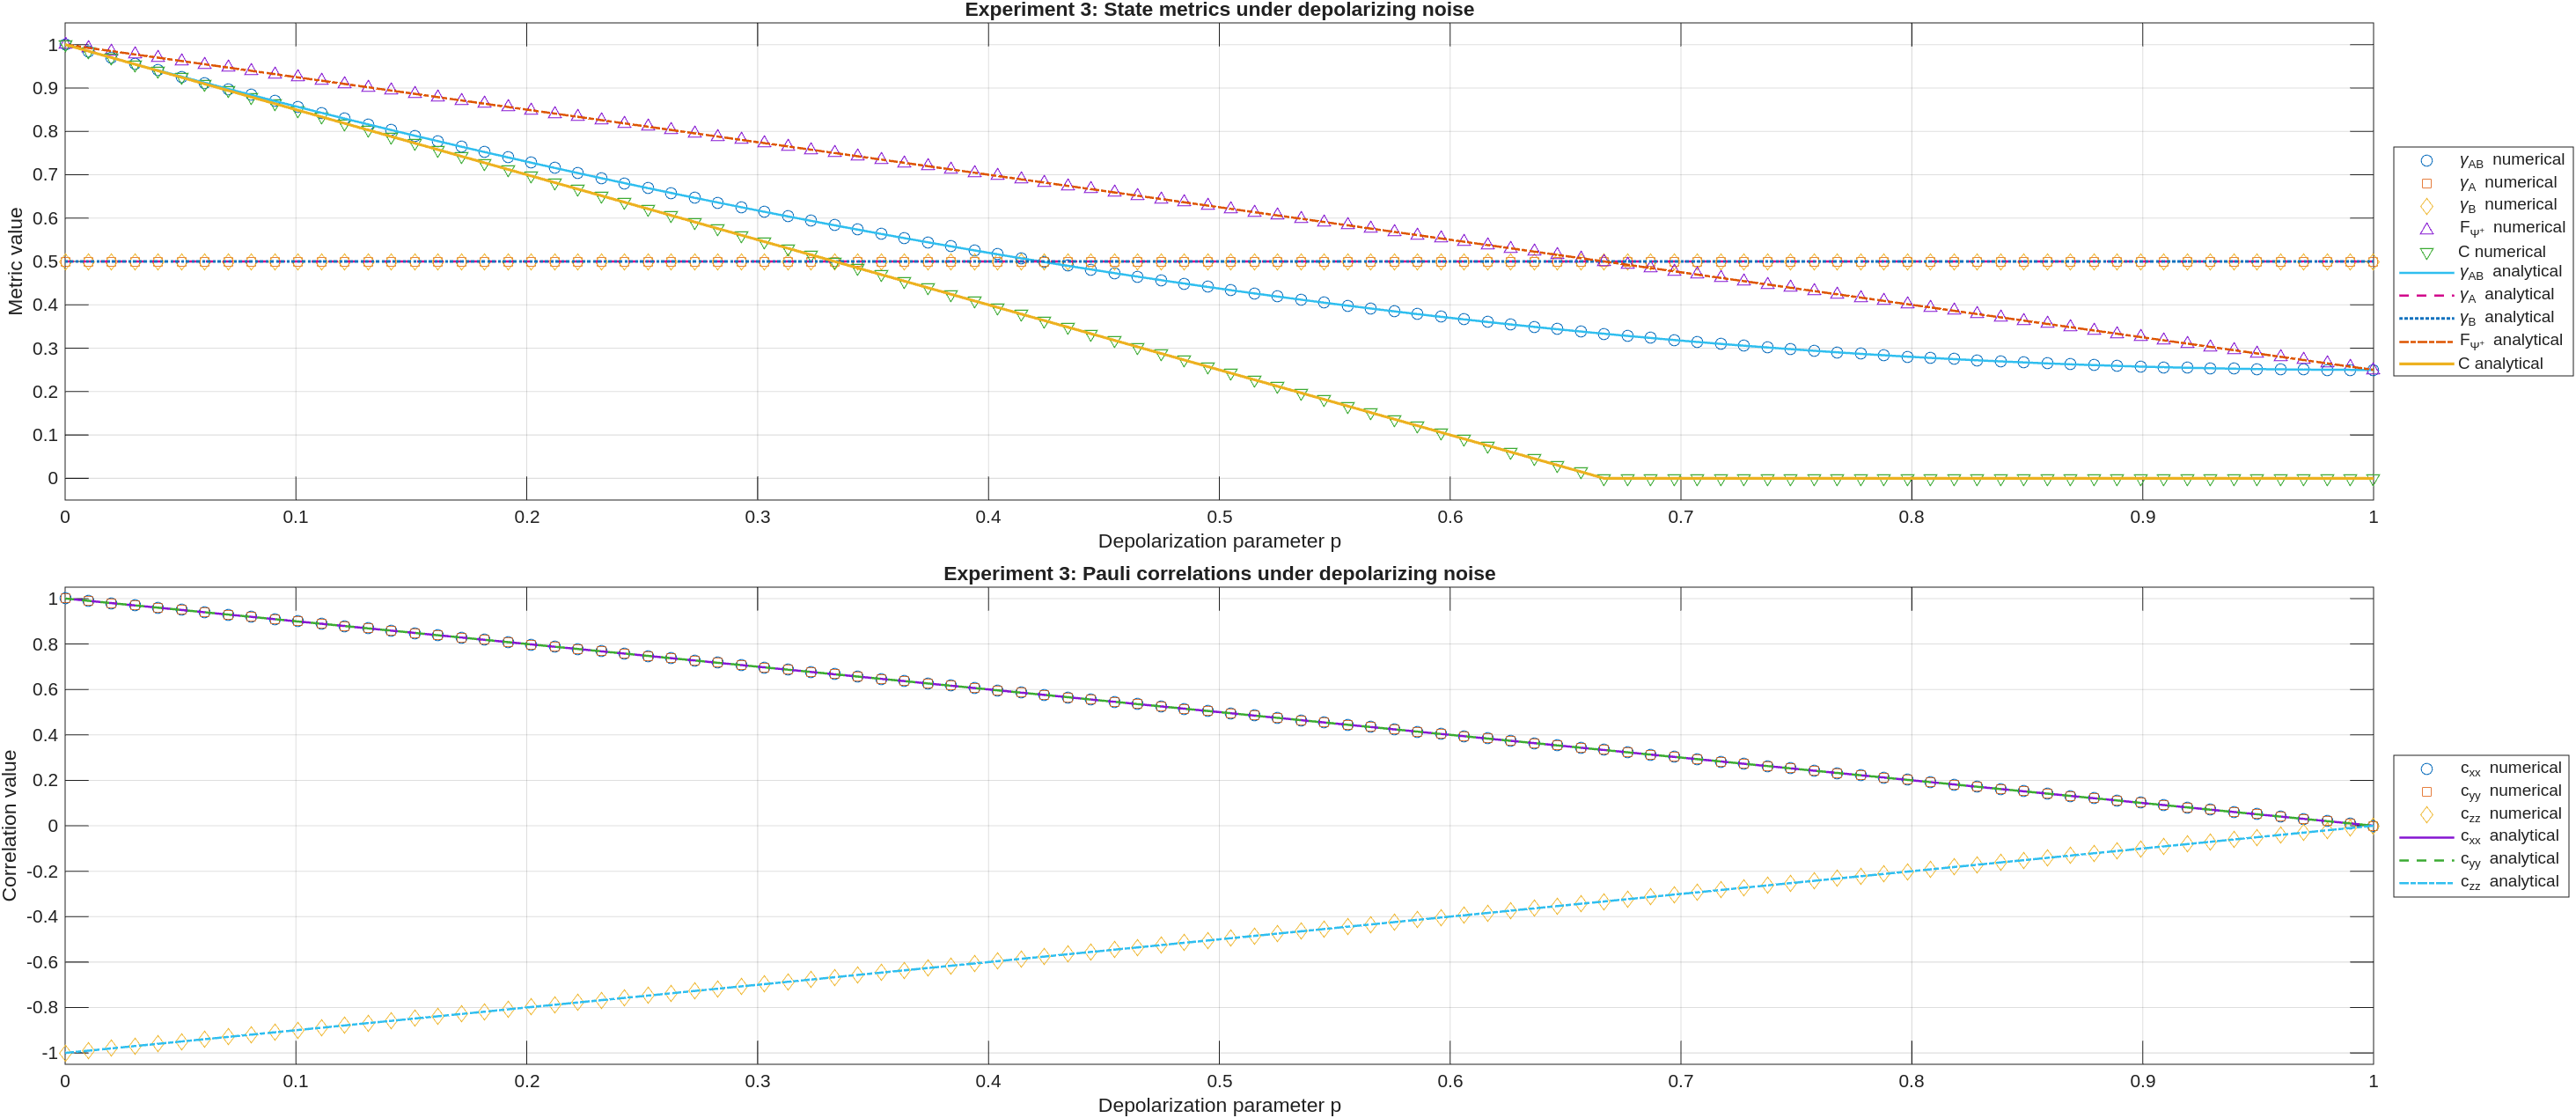
\includegraphics[width=\textwidth]{../Images/Experiment_3/experiment_3_depolarizing_channel_summary.png}
\caption{
Numerical and analytical behavior of purity, fidelity, concurrence, and correlations under the depolarizing channel. Agreement is exact up to numerical precision.
}
\label{fig:experiment3_depolarizing_summary}
\end{figure}

%--------------------------------------------------------
% Discussion
%--------------------------------------------------------

\subsubsection{Discussion}

This experiment validates the first non-unitary extension of the simulator.

Depolarization reduces global coherence and entanglement while leaving the reduced states maximally mixed. The different quantities exhibit distinct behaviors:
\begin{itemize}
\item purity decreases smoothly over the full interval;
\item concurrence exhibits threshold behavior, vanishing at \(p=2/3\);
\item correlations decay linearly in magnitude;
\item the full correlation tensor is uniformly contracted by the factor \(1-p\).
\end{itemize}

The numerical validation is consistent with the results of Experiment~2. In both experiments, the reduced states remain maximally mixed and the numerical errors remain at machine precision. However, the physical origin of mixedness is different. In Experiment~2, mixedness arises from averaging over unresolved phase realizations, while in Experiment~3 it is introduced directly by a non-unitary depolarizing channel.

This distinction is important: the random-phase ensemble preserves the structure associated with phase fluctuations, whereas the depolarizing channel isotropically suppresses the nontrivial two-qubit correlations by mixing the state with \(I_4/4\).

%--------------------------------------------------------
% Physical Interpretation
%--------------------------------------------------------

\subsubsection{Physical Interpretation}

The depolarizing channel provides an effective description of coherence loss when polarization becomes partially inaccessible due to unresolved physical mechanisms such as frequency dependence, temporal walk-off, or polarization-mode dispersion.

Its action drives the initial Bell state toward the maximally mixed state, progressively suppressing both correlations and entanglement.

Although not a complete microscopic model, this channel serves as a baseline for describing decoherence and establishes a reference against which more realistic fiber models can be compared.


%========================================================
% Subsection 5.4 — Experiment 4: CHSH Nonlocality
%========================================================

\newpage

\subsection{Experiment 4: CHSH Nonlocality}

%--------------------------------------------------------
% Objective
%--------------------------------------------------------

\subsubsection{Objective}

The objective of this experiment is to quantify the nonlocal correlations of the bipartite state through the Clauser--Horne--Shimony--Holt (CHSH) parameter.

\medskip

The experiment compares two physically different mechanisms:

\begin{itemize}
    \item deterministic phase evolution, described by local unitary transformations;
    \item depolarizing noise, described by an effective two-qubit quantum channel.
\end{itemize}

\medskip

The analysis distinguishes between two CHSH quantities:

\begin{itemize}
    \item \( S_{\mathrm{fixed}} \), computed using fixed laboratory measurement axes;
    \item \( S_{\max} \), computed from the correlation tensor and representing the maximal CHSH value achievable after optimizing the measurement axes.
\end{itemize}

\medskip

This distinction is essential because a reduction of \( S_{\mathrm{fixed}} \) does not necessarily imply a physical loss of nonlocality. It may also result from a misalignment between the fixed measurement axes and the rotated correlation tensor.

\medskip

%--------------------------------------------------------
% Model
%--------------------------------------------------------

\subsubsection{Model}

The reference state is the Bell state
\[
|\Psi^+\rangle
=
\frac{1}{\sqrt{2}}
\left(
|01\rangle + |10\rangle
\right).
\]

\medskip

Two families of states are analyzed.

\medskip

\textbf{Phase-evolved states.}

\[
|\psi(\theta)\rangle
=
\frac{1}{\sqrt{2}}
\left(
|01\rangle + e^{i\theta}|10\rangle
\right),
\]
obtained by applying a local phase unitary \( U_A(\theta) \otimes I_B \).

\medskip

\textbf{Depolarized states.}

\[
\rho(p)
=
(1-p)\rho_0
+
\frac{p}{4}I_4,
\]
where
\[
\rho_0 = |\Psi^+\rangle\langle\Psi^+|,
\qquad
p \in [0,1].
\]

\medskip

The fixed CHSH measurement settings are chosen to be optimal for \( |\Psi^+\rangle \) at \( \theta = 0 \), whose correlation tensor is
\[
T(0) =
\begin{pmatrix}
1 & 0 & 0 \\
0 & 1 & 0 \\
0 & 0 & -1
\end{pmatrix}.
\]

\medskip

The local axes are
\[
\mathbf{a}_1 =
\begin{pmatrix}
1 \\ 0 \\ 0
\end{pmatrix},
\qquad
\mathbf{a}_2 =
\begin{pmatrix}
0 \\ 1 \\ 0
\end{pmatrix},
\]
for subsystem \( A \), and
\[
\mathbf{b}_1 =
\frac{1}{\sqrt{2}}
\begin{pmatrix}
1 \\ 1 \\ 0
\end{pmatrix},
\qquad
\mathbf{b}_2 =
\frac{1}{\sqrt{2}}
\begin{pmatrix}
1 \\ -1 \\ 0
\end{pmatrix},
\]
for subsystem \( B \).

\medskip

The corresponding local Bloch-sphere geometry is shown in Fig.~\ref{fig:exp4_bloch_axes}.

\medskip

\begin{figure}[htbp]
    \centering
    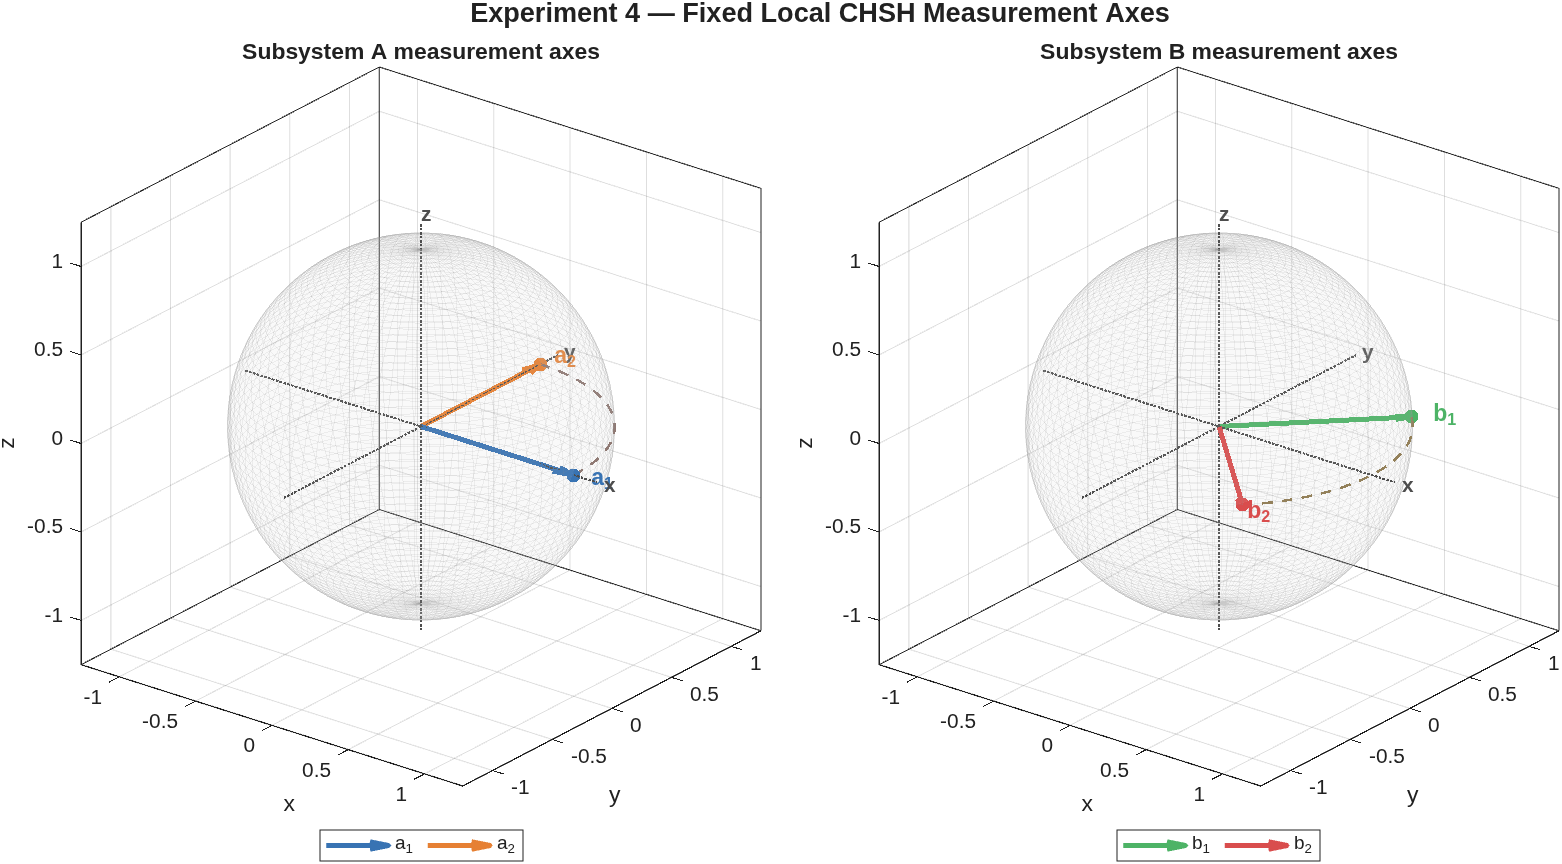
\includegraphics[width=0.9\textwidth]{../Images/Experiment_4/experiment_4_bloch_axes.png}
    \caption{Fixed local CHSH measurement axes represented on the Bloch spheres of subsystems \( A \) and \( B \). The left panel shows the analyzer directions \( \mathbf{a}_1 \) and \( \mathbf{a}_2 \), while the right panel shows \( \mathbf{b}_1 \) and \( \mathbf{b}_2 \). These axes define the fixed laboratory configuration used to compute \( S_{\mathrm{fixed}} \).}
    \label{fig:exp4_bloch_axes}
\end{figure}

\medskip

With these settings, \( S_{\mathrm{fixed}} \) represents the value measured by a fixed analyzer configuration, while \( S_{\max} \) represents the best value obtainable by adapting the analyzer axes to the state.

\medskip

%--------------------------------------------------------
% Analytical Predictions
%--------------------------------------------------------

\subsubsection{Analytical Predictions}

For the phase-evolved Bell state, the correlation tensor is rotated in the \( xy \)-plane:
\[
T(\theta)
=
\begin{pmatrix}
\cos\theta & -\sin\theta & 0 \\
\sin\theta & \cos\theta & 0 \\
0 & 0 & -1
\end{pmatrix}.
\]

\medskip

Using the fixed axes defined above, the CHSH value becomes
\[
S_{\mathrm{fixed}}(\theta)
=
2\sqrt{2}\cos\theta.
\]

\medskip

In the figure, the plotted quantity is \( |S_{\mathrm{fixed}}| \), since CHSH violation is determined by the magnitude condition
\[
|S| > 2.
\]

\medskip

The maximal CHSH value is instead independent of \( \theta \):
\[
S_{\max} = 2\sqrt{2}.
\]

\medskip

This expresses the fact that deterministic phase evolution is a local unitary transformation and therefore preserves the intrinsic nonlocal content of the Bell state.

\medskip

For the depolarizing channel, the correlation tensor is uniformly contracted:
\[
T(p) = (1-p)T(0).
\]

\medskip

Therefore,
\[
S_{\mathrm{fixed}}(p)
=
2\sqrt{2}(1-p),
\qquad
S_{\max}(p)
=
2\sqrt{2}(1-p).
\]

\medskip

The CHSH violation threshold is obtained from
\[
S_{\max}(p) > 2,
\]
which gives
\[
p < p_{\mathrm{CHSH}}
=
1 - \frac{1}{\sqrt{2}}
\simeq 0.2929.
\]

\medskip

%--------------------------------------------------------
% Numerical Results
%--------------------------------------------------------

\subsubsection{Numerical Results}

The numerical results are shown in Fig.~\ref{fig:exp4_chsh}.

\medskip

\begin{figure}[htbp]
    \centering
    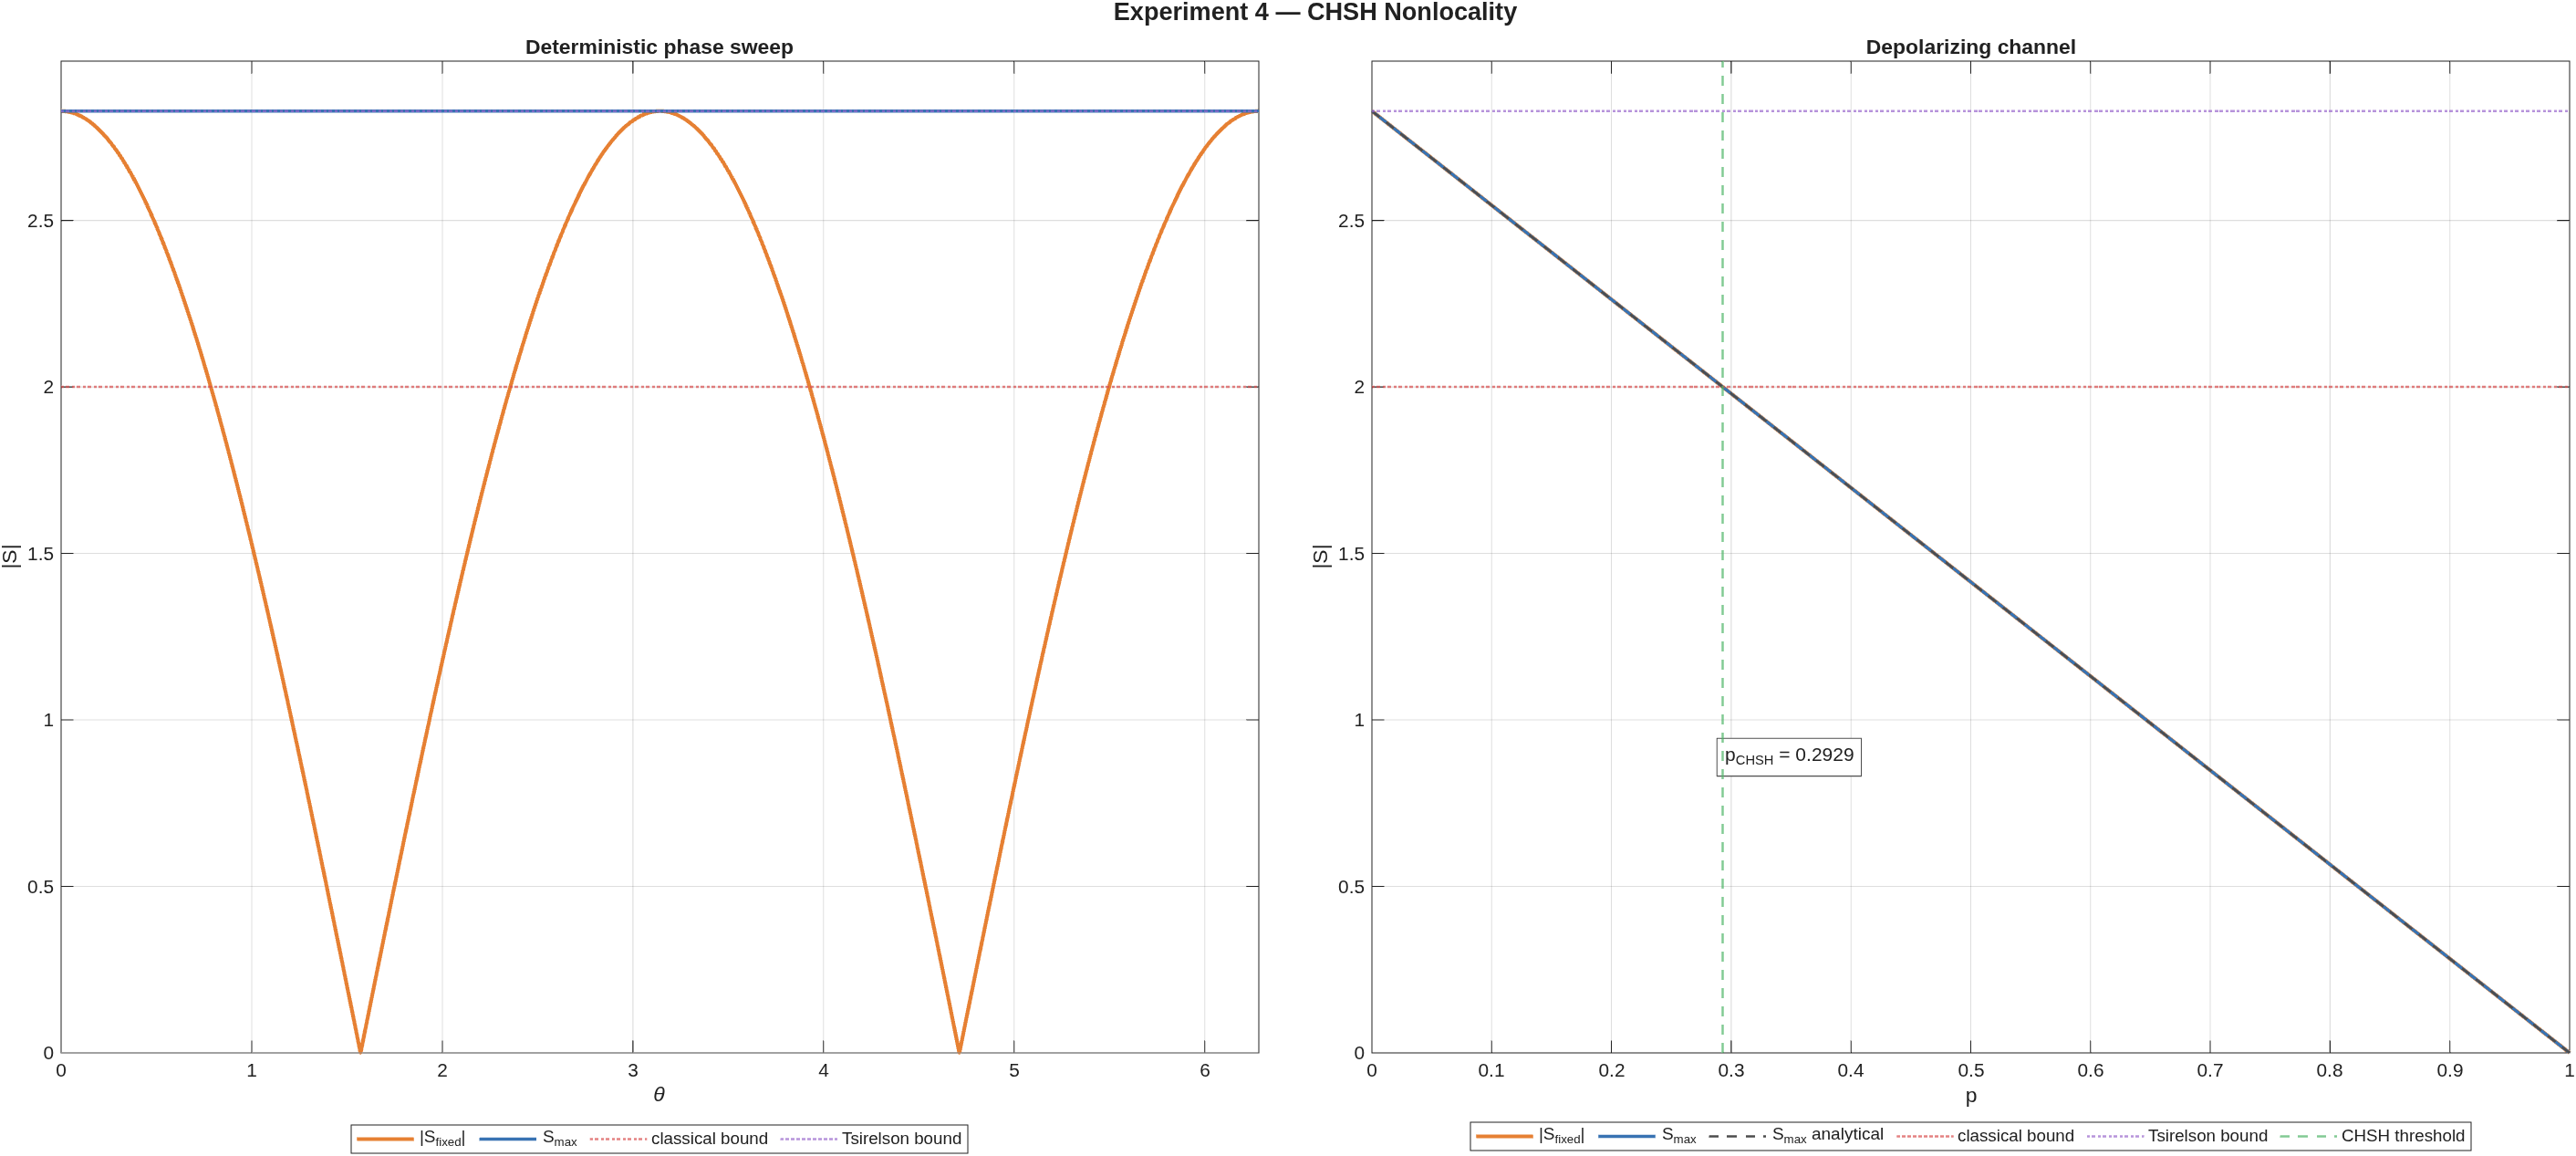
\includegraphics[width=0.9\textwidth]{../Images/Experiment_4/experiment_4_chsh_nonlocality_summary.png}
    \caption{CHSH behavior under deterministic phase evolution and depolarizing noise. The left panel shows \( |S_{\mathrm{fixed}}| \) and \( S_{\max} \) as functions of the phase \( \theta \). The right panel shows the corresponding quantities as functions of the depolarizing parameter \( p \). The red dotted line is the classical CHSH bound \( |S|=2 \), while the purple dotted line is the Tsirelson bound \( 2\sqrt{2} \).}
    \label{fig:exp4_chsh}
\end{figure}

\medskip

In the deterministic phase sweep, \( |S_{\mathrm{fixed}}| \) oscillates between zero and the Tsirelson bound. This behavior follows from the fixed measurement axes: as the phase \( \theta \) changes, the correlation tensor rotates relative to the laboratory analyzer directions.

\medskip

At the same time, \( S_{\max} \) remains constant and equal to \( 2\sqrt{2} \), confirming that the state remains maximally nonlocal when the measurement axes are allowed to adapt to the rotated tensor.

\medskip

In the depolarizing case, the numerical and analytical curves for \( S_{\max} \) overlap. Both \( |S_{\mathrm{fixed}}| \) and \( S_{\max} \) decrease linearly with \( p \), crossing the classical bound at \( p_{\mathrm{CHSH}} \simeq 0.2929 \).

\medskip

%--------------------------------------------------------
% Discussion
%--------------------------------------------------------

\subsubsection{Discussion}

The two panels of Fig.~\ref{fig:exp4_chsh} show two qualitatively different mechanisms.

\medskip

In the phase-evolution case, the state remains pure and maximally entangled for every value of \( \theta \). The oscillation of \( |S_{\mathrm{fixed}}| \) therefore does not represent a loss of entanglement or a loss of intrinsic nonlocality. Instead, it shows that fixed laboratory axes may become non-optimal when the fiber introduces a relative phase.

\medskip

This is why \( |S_{\mathrm{fixed}}| \) can fall below the classical bound, or even vanish, while \( S_{\max} \) remains fixed at the Tsirelson value. The apparent loss of CHSH violation is caused by measurement-axis mismatch.

\medskip

In the depolarizing case, the behavior is different. The channel reduces the magnitude of the correlation tensor itself. As a consequence, no change of measurement axes can recover the lost CHSH violation once \( p \) exceeds the threshold \( p_{\mathrm{CHSH}} \).

\medskip

Thus, \( S_{\mathrm{fixed}} \) is sensitive to both physical degradation and measurement misalignment, while \( S_{\max} \) isolates the maximal nonlocality still present in the state.

\medskip

%--------------------------------------------------------
% Physical Interpretation
%--------------------------------------------------------

\subsubsection{Physical Interpretation}

This experiment separates coherent fiber-induced transformations from incoherent degradation mechanisms.

\medskip

A deterministic relative phase acts as a local unitary transformation. Physically, this can originate from birefringence-induced phase accumulation between polarization components. Such an effect rotates the correlation tensor but does not reduce its singular values. Therefore, the nonlocal resource is preserved, even though a fixed analyzer configuration may fail to reveal it.

\medskip

Depolarization has a different physical meaning. It models the effective loss of polarization coherence produced by unresolved degrees of freedom, statistical fluctuations, or frequency-dependent propagation effects. In this case, the correlation tensor is not only rotated but contracted, and the available nonlocality is genuinely reduced.

\medskip

The comparison between \( S_{\mathrm{fixed}} \) and \( S_{\max} \) therefore provides an operational diagnostic. If \( S_{\mathrm{fixed}} \) changes while \( S_{\max} \) remains constant, the effect is compatible with coherent misalignment. If \( S_{\max} \) decreases, the state itself has lost nonlocal correlation strength.

\medskip

For the quantum fiber simulator, this distinction is important: a fiber-induced phase shift can hide CHSH violation from fixed laboratory measurements, whereas depolarizing effects represent an actual degradation of the entangled photon pair.


%========================================================
% APPENDICES
%========================================================

\appendix

\section*{Appendices}
\addcontentsline{toc}{section}{Appendices}

%========================================================
% APPENDIX A - Explicit Derivation of Reduced Density Operators and Comparison of Global States
%========================================================

\section{Explicit Derivation of Reduced Density Operators and Comparison of Global States}
\label{app:reduced_density_operators}

This appendix provides an explicit derivation of the reduced density operators for the phase-evolved Bell-like state and illustrates why identical local reduced states may correspond to different global physical situations.

We consider the two-qubit state
\[
|\psi(\theta)\rangle = \frac{|01\rangle + e^{i\theta}|10\rangle}{\sqrt{2}},
\]
in the computational basis
\[
\{|00\rangle, |01\rangle, |10\rangle, |11\rangle\}.
\]

Its vector representation is
\[
|\psi(\theta)\rangle =
\frac{1}{\sqrt{2}}
\begin{pmatrix}
0 \\
1 \\
e^{i\theta} \\
0
\end{pmatrix}.
\]

The corresponding density operator is
\[
\rho_{AB}(\theta) = |\psi(\theta)\rangle\langle\psi(\theta)|,
\]
which in matrix form reads
\[
\rho_{AB}(\theta)
=
\frac{1}{2}
\begin{pmatrix}
0 & 0 & 0 & 0 \\
0 & 1 & e^{-i\theta} & 0 \\
0 & e^{i\theta} & 1 & 0 \\
0 & 0 & 0 & 0
\end{pmatrix}.
\]

The reduced density operator of subsystem \(A\) is obtained via the partial trace
\[
\rho_A(\theta) = \mathrm{Tr}_B(\rho_{AB}(\theta)).
\]

Using
\[
\rho_A(\theta)
=
\sum_{b=0}^{1}
(I_A \otimes \langle b|)\,\rho_{AB}(\theta)\,(I_A \otimes |b\rangle),
\]
one evaluates the contributions term by term.

Diagonal terms yield
\[
\mathrm{Tr}_B(|01\rangle\langle 01|) = |0\rangle\langle 0|,
\qquad
\mathrm{Tr}_B(|10\rangle\langle 10|) = |1\rangle\langle 1|.
\]

Off-diagonal terms vanish:
\[
\mathrm{Tr}_B(|01\rangle\langle 10|) = 0,
\qquad
\mathrm{Tr}_B(|10\rangle\langle 01|) = 0,
\]
due to orthogonality in subsystem \(B\).

Summing all contributions,
\[
\rho_A(\theta)
=
\frac{1}{2}|0\rangle\langle 0|
+
\frac{1}{2}|1\rangle\langle 1|
=
\frac{I}{2}.
\]

By symmetry,
\[
\rho_B(\theta) = \frac{I}{2}.
\]

Thus, although the global state depends on the phase \( \theta \), the reduced states do not. The phase appears only in off-diagonal coherence terms, which are eliminated by the partial trace.

In particular, for \( \theta = 0 \),
\[
|\Psi^+\rangle = \frac{|01\rangle + |10\rangle}{\sqrt{2}},
\]
and one obtains the same reduced states,
\[
\rho_A = \rho_B = \frac{I}{2}.
\]


To clarify the meaning of this result, consider the classical mixture
\[
\rho^{(\mathrm{class})}
=
\frac{1}{2}|0\rangle\langle 0|
+
\frac{1}{2}|1\rangle\langle 1|
=
\frac{I}{2}.
\]

At the local level,
\[
\rho_A^{(\mathrm{ent})} = \rho^{(\mathrm{class})},
\]
and therefore, for any observable \(O_A\),
\[
\mathrm{Tr}(\rho^{(\mathrm{class})} O_A)
=
\mathrm{Tr}(\rho_A^{(\mathrm{ent})} O_A).
\]

Hence, local measurements cannot distinguish classical mixtures from reductions of entangled states.

At the global level, the distinction becomes evident. Consider the separable state
\[
\rho_{AB}^{(\mathrm{sep})}
=
\frac{1}{2}|01\rangle\langle 01|
+
\frac{1}{2}|10\rangle\langle 10|.
\]

It has the same reduced states,
\[
\mathrm{Tr}_B(\rho_{AB}^{(\mathrm{sep})}) = \frac{I}{2},
\qquad
\mathrm{Tr}_A(\rho_{AB}^{(\mathrm{sep})}) = \frac{I}{2},
\]
but lacks the coherence terms present in \( \rho_{AB}(\theta) \).

This difference is reflected in global quantities. For the entangled state,
\[
\gamma(\rho_{AB}(\theta)) = 1,
\]
whereas for the separable state,
\[
\gamma(\rho_{AB}^{(\mathrm{sep})}) = \frac{1}{2}.
\]

A second distinction appears in correlations:
\[
\langle \sigma_x \otimes \sigma_x \rangle = \cos\theta, \qquad
\langle \sigma_y \otimes \sigma_y \rangle = \cos\theta,
\]
for the entangled state, while
\[
\langle \sigma_x \otimes \sigma_x \rangle = 0, \qquad
\langle \sigma_y \otimes \sigma_y \rangle = 0,
\]
for the separable mixture.

Thus, states with identical reduced density operators may differ fundamentally at the global level. Reduced states encode all locally accessible information, but do not capture global coherence or bipartite entanglement.

%==============================================================
% APPENDIX B - Derivation of Fidelity for a Pure Reference State
%========================================================

\section{Derivation of Fidelity for a Pure Reference State}


We derive the simplified expression for the fidelity when one of the states is pure, and justify the algebraic properties used in the reduction.

\medskip

Let $\rho$ be a density operator on a finite-dimensional Hilbert space, and let
\[
\sigma = |\psi\rangle\langle\psi|
\]
be a pure-state density operator, with $|\psi\rangle$ normalized:
\[
\langle \psi | \psi \rangle = 1.
\]

By construction, $\sigma$ is Hermitian,
\[
\sigma^\dagger = \sigma,
\]
positive semidefinite,
\[
\langle \chi | \sigma | \chi \rangle \ge 0
\quad \text{for all } |\chi\rangle,
\]
and satisfies
\[
\operatorname{Tr}(\sigma) = 1.
\]
Moreover, it is a rank-one operator, since it projects onto the one-dimensional subspace spanned by $|\psi\rangle$.

\medskip

The general definition of fidelity is
\[
F(\rho,\sigma)
=
\left(\operatorname{Tr}\sqrt{\sqrt{\rho}\,\sigma\,\sqrt{\rho}}\right)^2.
\]

Substituting $\sigma = |\psi\rangle\langle\psi|$, one obtains
\[
\sqrt{\rho}\,\sigma\,\sqrt{\rho}
=
\sqrt{\rho}\,|\psi\rangle\langle\psi|\,\sqrt{\rho}.
\]

Define the vector
\[
|\phi\rangle = \sqrt{\rho}\,|\psi\rangle.
\]
Then the operator becomes
\[
\sqrt{\rho}\,\sigma\,\sqrt{\rho}
=
|\phi\rangle\langle\phi|.
\]

This is again a rank-one operator, provided $|\phi\rangle \neq 0$.

\medskip

We now compute the square root of this operator. Since
\[
|\phi\rangle\langle\phi|
\]
is positive semidefinite and rank one, its only nonzero eigenvalue is
\[
\lambda = \langle \phi | \phi \rangle.
\]

Thus, its spectral decomposition is
\[
|\phi\rangle\langle\phi|
=
\lambda\,|\hat{\phi}\rangle\langle\hat{\phi}|,
\]
where
\[
|\hat{\phi}\rangle = \frac{|\phi\rangle}{\|\phi\|}.
\]

The square root is then
\[
\sqrt{|\phi\rangle\langle\phi|}
=
\sqrt{\lambda}\,|\hat{\phi}\rangle\langle\hat{\phi}|.
\]

Taking the trace,
\[
\operatorname{Tr}\sqrt{|\phi\rangle\langle\phi|}
=
\sqrt{\lambda}.
\]

Therefore,
\[
F(\rho,\sigma)
=
\lambda
=
\langle \phi | \phi \rangle.
\]

Recalling the definition of $|\phi\rangle$,
\[
\lambda
=
\langle \psi | \rho | \psi \rangle.
\]

\medskip

We conclude that when $\sigma = |\psi\rangle\langle\psi|$ is a pure state, the fidelity reduces to
\[
F(\rho,|\psi\rangle\langle\psi|)
=
\langle \psi | \rho | \psi \rangle.
\]

\medskip

This result justifies the simplified expression used in Section 4.3. It also shows that the fidelity corresponds to the expectation value of the projector onto $|\psi\rangle$, providing a direct probabilistic interpretation as the probability of obtaining the outcome $|\psi\rangle$ in a projective measurement.


%========================================================
% Appendix C — Concurrence and Reduced Density Operators
%========================================================

\section{Derivations for Concurrence and Reduced Density Operators}

This appendix collects the algebraic derivations leading to the relation between concurrence and reduced density operators for pure two-qubit states.

Let
\[
|\psi\rangle
=
a|00\rangle + b|01\rangle + c|10\rangle + d|11\rangle
\]
be a normalized two-qubit state.

Introduce the coefficient matrix
\[
A_\psi =
\begin{pmatrix}
a & b\\
c & d
\end{pmatrix},
\]
so that
\[
|\psi\rangle
=
\sum_{i,j=0}^{1} (A_\psi)_{ij}\,|i\rangle \otimes |j\rangle.
\]


The global density operator is
\[
\rho_{AB} = |\psi\rangle\langle\psi|.
\]

Expanding in the computational basis,
\[
\rho_{AB}
=
\sum_{i,j,k,l}
(A_\psi)_{ij}(A_\psi)^*_{kl}
\;
|i\rangle\langle k|
\otimes
|j\rangle\langle l|.
\]

The reduced density operator on subsystem \(A\) is
\[
\rho_A = \operatorname{Tr}_B(\rho_{AB}).
\]

Applying the partial trace,
\[
\rho_A
=
\sum_{i,j,k,l}
(A_\psi)_{ij}(A_\psi)^*_{kl}
\left(
\sum_v \langle v|j\rangle \langle l|v\rangle
\right)
|i\rangle\langle k|.
\]

Using
\[
\sum_v \langle v|j\rangle \langle l|v\rangle = \delta_{jl},
\]
one obtains
\[
\rho_A
=
\sum_{i,k,j}
(A_\psi)_{ij}(A_\psi)^*_{kj}
\,|i\rangle\langle k|.
\]

Thus, in matrix form,
\[
\rho_A = A_\psi A_\psi^\dagger.
\]

Similarly,
\[
\rho_B = A_\psi^\dagger A_\psi.
\]

For pure states, concurrence is defined as
\[
C(|\psi\rangle)
=
\left|
\langle \psi | (\sigma_y \otimes \sigma_y)\,|\psi^*\rangle
\right|.
\]

With
\[
|\psi\rangle =
\begin{pmatrix}
a\\ b\\ c\\ d
\end{pmatrix},
\qquad
|\psi^*\rangle =
\begin{pmatrix}
a^*\\ b^*\\ c^*\\ d^*
\end{pmatrix},
\]
and
\[
\sigma_y \otimes \sigma_y =
\begin{pmatrix}
0 & 0 & 0 & -1\\
0 & 0 & 1 & 0\\
0 & 1 & 0 & 0\\
-1 & 0 & 0 & 0
\end{pmatrix},
\]
one obtains
\[
(\sigma_y \otimes \sigma_y)|\psi^*\rangle
=
\begin{pmatrix}
- d^*\\
c^*\\
b^*\\
- a^*
\end{pmatrix}.
\]

Taking the inner product,
\[
\langle \psi | (\sigma_y \otimes \sigma_y)|\psi^*\rangle
=
2(ad - bc)^*,
\]
and therefore
\[
C(|\psi\rangle)=2|ad-bc|.
\]

Using
\[
\det(A_\psi) = ad - bc,
\]
this becomes
\[
C(|\psi\rangle)=2|\det(A_\psi)|.
\]

From
\[
\rho_A = A_\psi A_\psi^\dagger,
\]
it follows that
\[
\det(\rho_A)
=
\det(A_\psi)\det(A_\psi^\dagger)
=
|\det(A_\psi)|^2.
\]

Thus,
\[
C(|\psi\rangle)=2\sqrt{\det(\rho_A)}.
\]

An identical relation holds for \(\rho_B\).

For a single-qubit density operator,
\[
\operatorname{Tr}(\rho)=1,
\]
and
\[
\gamma(\rho)=\operatorname{Tr}(\rho^2).
\]

One has the identity
\[
\det(\rho)
=
\frac{1 - \gamma(\rho)}{2}.
\]

Substituting,
\[
C(|\psi\rangle)
=
\sqrt{2\left(1 - \gamma(\rho_A)\right)}.
\]

This shows explicitly that, for pure bipartite states, entanglement is directly encoded in the mixedness of the reduced subsystems.

%========================================================
% Appendix D — Analytical Derivations for Experiment 3: Depolarizing Channel
%========================================================

\section{Analytical Derivations for Experiment 3: Depolarizing Channel}

This appendix derives the analytical expressions used in Experiment~3 for the family of two-qubit states obtained by applying the depolarizing channel to the Bell state \( |\Psi^+\rangle \).

We consider the reference Bell state
\[
|\Psi^+\rangle = \frac{|01\rangle + |10\rangle}{\sqrt{2}},
\]
with density operator
\[
\rho_0 = |\Psi^+\rangle\langle\Psi^+|.
\]

The depolarized family is defined as
\[
\rho(p)
=
(1-p)\rho_0 + \frac{p}{4}I_4,
\qquad
p \in [0,1].
\]

%--------------------------------------------------------
% Density matrix form
%--------------------------------------------------------

\subsection*{Density matrix form}

In the computational basis
\[
\{|00\rangle, |01\rangle, |10\rangle, |11\rangle\},
\]
the projector onto \( |\Psi^+\rangle \) is
\[
\rho_0
=
\begin{pmatrix}
0 & 0 & 0 & 0\\
0 & \frac12 & \frac12 & 0\\
0 & \frac12 & \frac12 & 0\\
0 & 0 & 0 & 0
\end{pmatrix}.
\]

Therefore,
\[
\rho(p)
=
\begin{pmatrix}
\frac{p}{4} & 0 & 0 & 0\\
0 & \frac12-\frac{p}{4} & \frac{1-p}{2} & 0\\
0 & \frac{1-p}{2} & \frac12-\frac{p}{4} & 0\\
0 & 0 & 0 & \frac{p}{4}
\end{pmatrix}.
\]

%--------------------------------------------------------
% Global purity
%--------------------------------------------------------

\subsection*{Global purity}

The global purity is
\[
\gamma_{AB}(p) = \operatorname{Tr}\!\left(\rho(p)^2\right).
\]

Since \( \rho_0 \) is a rank-one projector and \( I_4/4 \) is proportional to the identity, the Bell-state direction remains an eigenvector of \( \rho(p) \), with eigenvalue
\[
\lambda_1 = 1-\frac{3p}{4}.
\]
The three orthogonal directions have eigenvalues
\[
\lambda_2=\lambda_3=\lambda_4=\frac{p}{4}.
\]

Hence,
\[
\gamma_{AB}(p)
=
\left(1-\frac{3p}{4}\right)^2
+
3\left(\frac{p}{4}\right)^2
=
1-\frac{3}{2}p+\frac{3}{4}p^2.
\]

%--------------------------------------------------------
% Reduced density operators and reduced purities
%--------------------------------------------------------

\subsection*{Reduced density operators and reduced purities}

For the Bell state,
\[
\operatorname{Tr}_B(\rho_0)
=
\operatorname{Tr}_A(\rho_0)
=
\frac{I_2}{2}.
\]

Moreover,
\[
\operatorname{Tr}_B\!\left(\frac{I_4}{4}\right)
=
\operatorname{Tr}_A\!\left(\frac{I_4}{4}\right)
=
\frac{I_2}{2}.
\]

By linearity,
\[
\rho_A(p)
=
\operatorname{Tr}_B(\rho(p))
=
(1-p)\frac{I_2}{2}
+
p\frac{I_2}{2}
=
\frac{I_2}{2},
\]
and similarly,
\[
\rho_B(p)=\frac{I_2}{2}.
\]

Therefore,
\[
\gamma_A(p)
=
\gamma_B(p)
=
\operatorname{Tr}\!\left[\left(\frac{I_2}{2}\right)^2\right]
=
\frac{1}{2}.
\]

%--------------------------------------------------------
% Fidelity with respect to the reference Bell state
%--------------------------------------------------------

\subsection*{Fidelity with respect to \texorpdfstring{$|\Psi^+\rangle$}{|Psi+>}}

Since the reference state is pure,
\[
F_{\Psi^+}(p)
=
\langle\Psi^+|\rho(p)|\Psi^+\rangle.
\]

Substituting \( \rho(p) \),
\[
F_{\Psi^+}(p)
=
(1-p)\langle\Psi^+|\rho_0|\Psi^+\rangle
+
\frac{p}{4}\langle\Psi^+|I_4|\Psi^+\rangle.
\]

Since
\[
\langle\Psi^+|\rho_0|\Psi^+\rangle = 1,
\qquad
\langle\Psi^+|I_4|\Psi^+\rangle = 1,
\]
one obtains
\[
F_{\Psi^+}(p)
=
1-\frac{3}{4}p.
\]

%--------------------------------------------------------
% Concurrence
%--------------------------------------------------------

\subsection*{Concurrence}

The family \( \rho(p) \) is Bell-diagonal. Its concurrence is
\[
C(p)
=
\max\left(0,\,2\lambda_{\max}-1\right),
\]
where \( \lambda_{\max} \) is the largest Bell-basis eigenvalue.

In the present case,
\[
\lambda_{\max}
=
1-\frac{3p}{4},
\]
and therefore
\[
C(p)
=
\max\left(0,\,1-\frac{3p}{2}\right).
\]

The concurrence vanishes when
\[
1-\frac{3p}{2}=0,
\qquad
p=\frac{2}{3},
\]
which identifies the separability threshold of the depolarized family.

%--------------------------------------------------------
% Pauli correlations
%--------------------------------------------------------

\subsection*{Pauli correlations}

The aligned Pauli correlations are
\[
c_{ii}(p)
=
\operatorname{Tr}\!\left[\rho(p)(\sigma_i\otimes\sigma_i)\right],
\qquad
i\in\{x,y,z\}.
\]

Using linearity,
\[
c_{ii}(p)
=
(1-p)\operatorname{Tr}\!\left[\rho_0(\sigma_i\otimes\sigma_i)\right]
+
\frac{p}{4}\operatorname{Tr}\!\left[I_4(\sigma_i\otimes\sigma_i)\right].
\]

Since \( \sigma_i\otimes\sigma_i \) is traceless,
\[
\operatorname{Tr}\!\left[I_4(\sigma_i\otimes\sigma_i)\right]
=
0,
\]
and therefore
\[
c_{ii}(p)=(1-p)c_{ii}(0).
\]

For \( |\Psi^+\rangle \),
\[
c_{xx}(0)=1,
\qquad
c_{yy}(0)=1,
\qquad
c_{zz}(0)=-1.
\]

Hence,
\[
c_{xx}(p)=1-p,
\qquad
c_{yy}(p)=1-p,
\qquad
c_{zz}(p)=-(1-p).
\]

%--------------------------------------------------------
% Summary
%--------------------------------------------------------

\subsection*{Summary of analytical expressions}

Collecting the results,
\[
\boxed{
\begin{aligned}
\gamma_{AB}(p) &= 1-\frac{3}{2}p+\frac{3}{4}p^2, \\
\gamma_A(p) &= \gamma_B(p)=\frac12, \\
F_{\Psi^+}(p) &= 1-\frac34 p, \\
C(p) &= \max\left(0,\,1-\frac32 p\right), \\
c_{xx}(p) &= 1-p,\qquad
c_{yy}(p)=1-p,\qquad
c_{zz}(p)=-(1-p).
\end{aligned}
}
\]

These expressions are used as analytical references for the numerical validation of Experiment~3.


%========================================================
% REFERENCES
%========================================================

\begin{thebibliography}{9}

\bibitem{NielsenChuang}
M.~A.~Nielsen and I.~L.~Chuang,  
\textit{Quantum Computation and Quantum Information},  
Cambridge University Press, 2000.

\bibitem{James2001}
D.~F.~V.~James, P.~G.~Kwiat, W.~J.~Munro, and A.~G.~White,  
``Measurement of qubits,''  
\textit{Physical Review A}, \textbf{64}, 052312 (2001).

\end{thebibliography}

\end{document}